\documentclass[aspectratio=169]{beamer}
\usepackage{new-mysymb}
\usepackage{xcolor}
\usepackage{varwidth}
\usepackage{tikz}
\usetikzlibrary{calc}
\usepackage{empheq}
\usepackage{amsmath}
\usepackage{textpos}
\setbeamertemplate{footline}[frame number]
\setbeamertemplate{navigation symbols}{}
\definecolor{lightblue}{rgb}{0.68, 0.85, 0.9}
\definecolor{lightred}{rgb}{1, 0.7, 0.7}
\definecolor{lightpurple}{rgb}{0.8,0.6,1.0}
\definecolor{darkgreen}{RGB}{144, 238, 144}
\usepackage[most]{tcolorbox}
\newtcolorbox{graybox}[2][]{%
  enhanced,
  colback=white!10,
  colframe=black!60,
  boxrule=0.8pt,
  boxsep=1pt,
  top=5pt,
  bottom=1pt,
  arc=2pt,
  left=6pt, right=6pt, top=5pt, bottom=1pt,
  attach boxed title to top left={xshift=0.5em, yshift=-2mm},
  boxed title style={colback=gray!30, colframe=gray!60, boxrule=0pt},
  fonttitle=\bfseries,
  coltitle=black,
  title={#2},
  #1
}

% commands
\newcommand{\bvx}{\bar{\vx}}
\newcommand{\deltavx}{\delta\vx}
\newcommand{\vPhi}{\boldsymbol{\Phi}}
\newcommand{\vPsi}{\boldsymbol{\Psi}}
\newcommand{\vkappa}{\boldsymbol{\kappa}}
\newcommand{\tvkappa}{\tilde{\boldsymbol{\kappa}}}
\newcommand{\vTheta}{\boldsymbol{\Theta}}
\newcommand{\vtheta}{\boldsymbol{\theta}}
\newcommand{\vzero}{\boldsymbol{0}}
\newcommand{\vlambda}{\boldsymbol{\lambda}}
\newcommand{\vcD}{\boldsymbol{\mathcal{D}}}
\newcommand{\vnu}{\boldsymbol{\nu}}
\newcommand{\bvu}{\bar{\mathbf{u}}}
\newcommand{\vXi}{\boldsymbol{\Xi}}
\newcommand{\vbeta}{\boldsymbol{\beta}}
\newcommand{\vLambda}{\boldsymbol{\Lambda}}
\newcommand{\redvTheta}{\textcolor{red}{\boldsymbol{\Theta}}}
\newcommand{\vomega}{\boldsymbol{\omega}}
\newcommand{\vcQ}{\boldsymbol{\mathcal{Q}}}
\newcommand{\vcH}{\boldsymbol{\mathcal{H}}}
\newcommand{\redvomega}{\textcolor{red}{\boldsymbol{\omega}}}
\newcommand{\redvbeta}{\textcolor{red}{\boldsymbol{\beta}}}
\newcommand{\redvB}{\textcolor{red}{\mathbf{B}}}
\newcommand{\vcF}{\boldsymbol{\mathcal{F}}}
\newcommand{\vmu}{\boldsymbol{\mu}}
\newcommand{\redTheta}{\textcolor{red}{\Theta}}
\newcommand{\valpha}{\boldsymbol{\alpha}}
\newcommand{\vOmega}{\boldsymbol{\Omega}}
\newcommand{\deltavu}{\delta\mathbf{u}}


\title[]{A Unified Control-Theoretic Framework for Physics-Infused Reduced-Order Modeling and Optimal Closed-Loop Control}
\subtitle{}
\author[]{Carlos A. Vargas Venegas}

\institute{}

\begin{document}

\maketitle


% part 1: introduction and objectives
\begin{frame}{Content Overview}
  \footnotesize
    \begin{enumerate}
        \item<2-> Motivation, Background, and Objectives
        \visible<3->{
        \begin{itemize}
            {\footnotesize
            \item The Impossible Trinity of Modeling (ITM)
            \item The Impossible Trinity of Optimal Control (ITOC)}
        \end{itemize}}
        \item<4-> Addressing the ITM
        \item<5-> Unified Control-Theoretic Training
        \item<6-> Addressing the ITOC
        \item<7-> Conclusions and Future Work
    \end{enumerate}
\end{frame}

\section{Motivation, Background, and Objectives}

\begin{frame}{Content Overview}
  \footnotesize
    \begin{enumerate}
        \item \colorbox{yellow!70}{\textbf{Motivation, Background, and Objectives}}
        \item \textcolor{gray!50}{Addressing the Impossible Trinity of Modeling (ITM)}
        \item \textcolor{gray!50}{Unified Control-Theoretic Training}
        \item \textcolor{gray!50}{Addressing the Impossible Trinity of Optimal Control (ITOC)}
        \item \textcolor{gray!50}{Conclusions and Future Work}
    \end{enumerate}
\end{frame}

% \begin{frame}{\large Motivation: Simulation and Control of Hypersonic Systems}
%     \footnotesize
%     \begin{columns}
%         \begin{column}{0.6\textwidth}
%             \centering
%             \only<1>{
%                 \begin{figure}
%                     \centering
%                     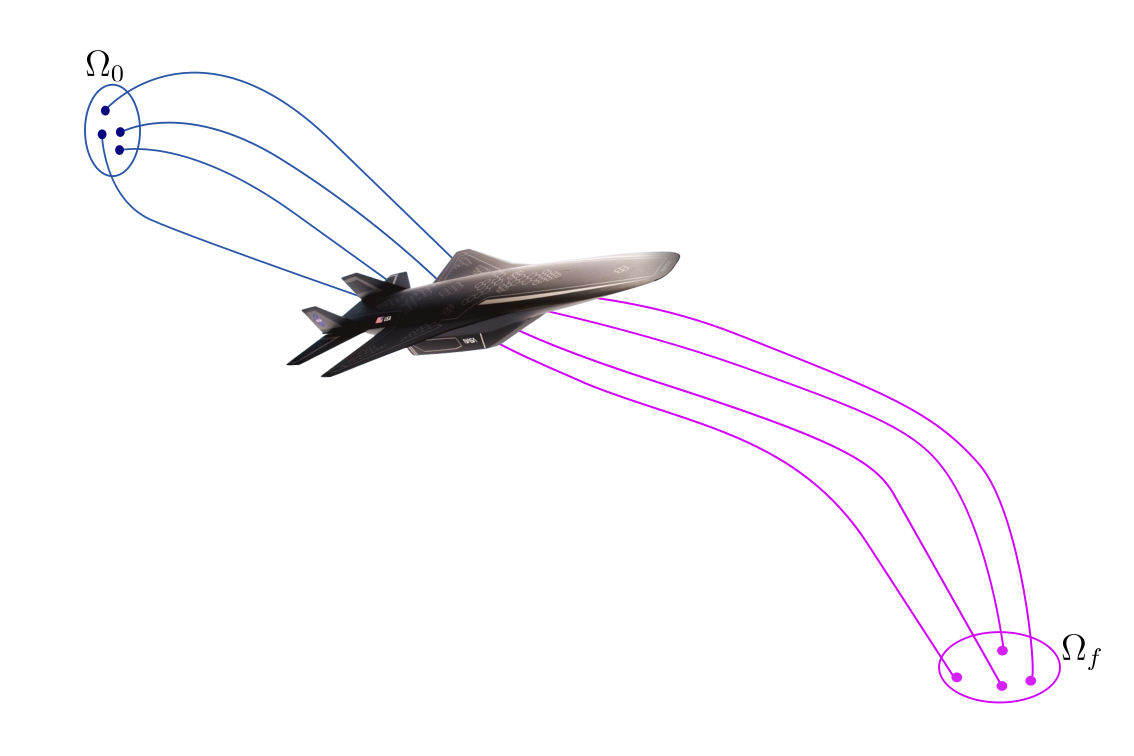
\includegraphics[width=0.9\textwidth]{../figs/introduction/motivating_example_1.png}
%                 \end{figure}}
%             \only<2>{
%                 \begin{figure}
%                     \centering
%                     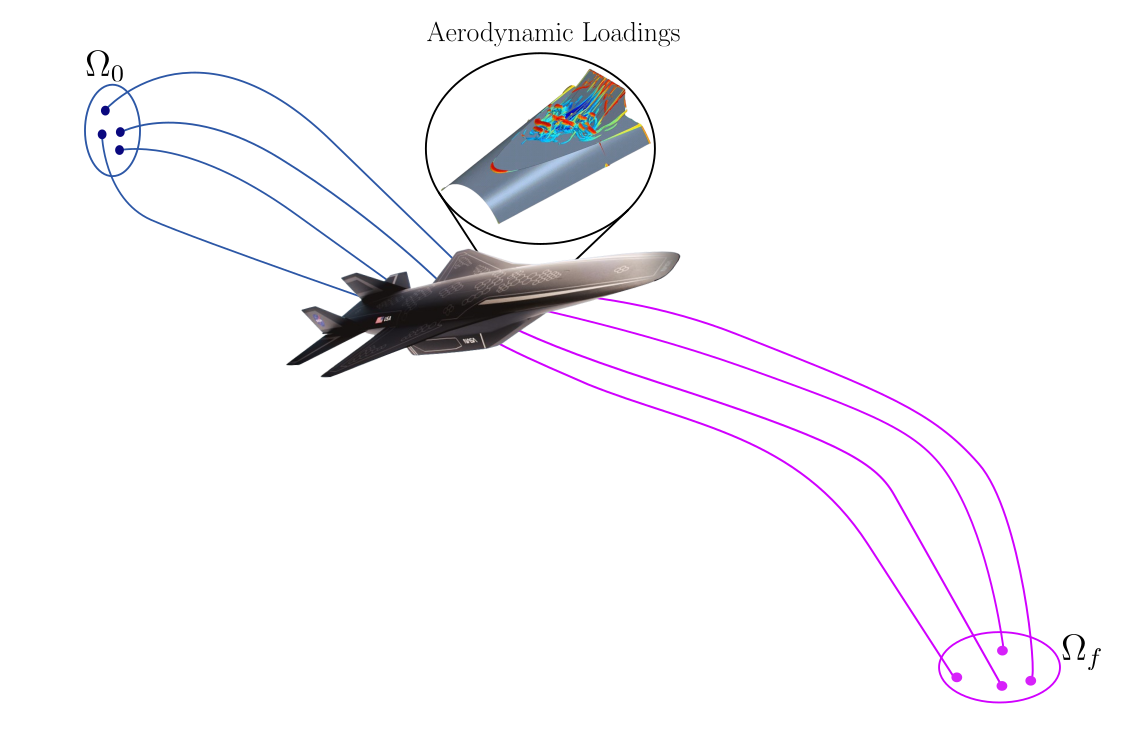
\includegraphics[width=0.9\textwidth]{../figs/introduction/motivating_example_2.png}
%                 \end{figure}}
%             \only<3>{
%                 \begin{figure}
%                     \centering
%                     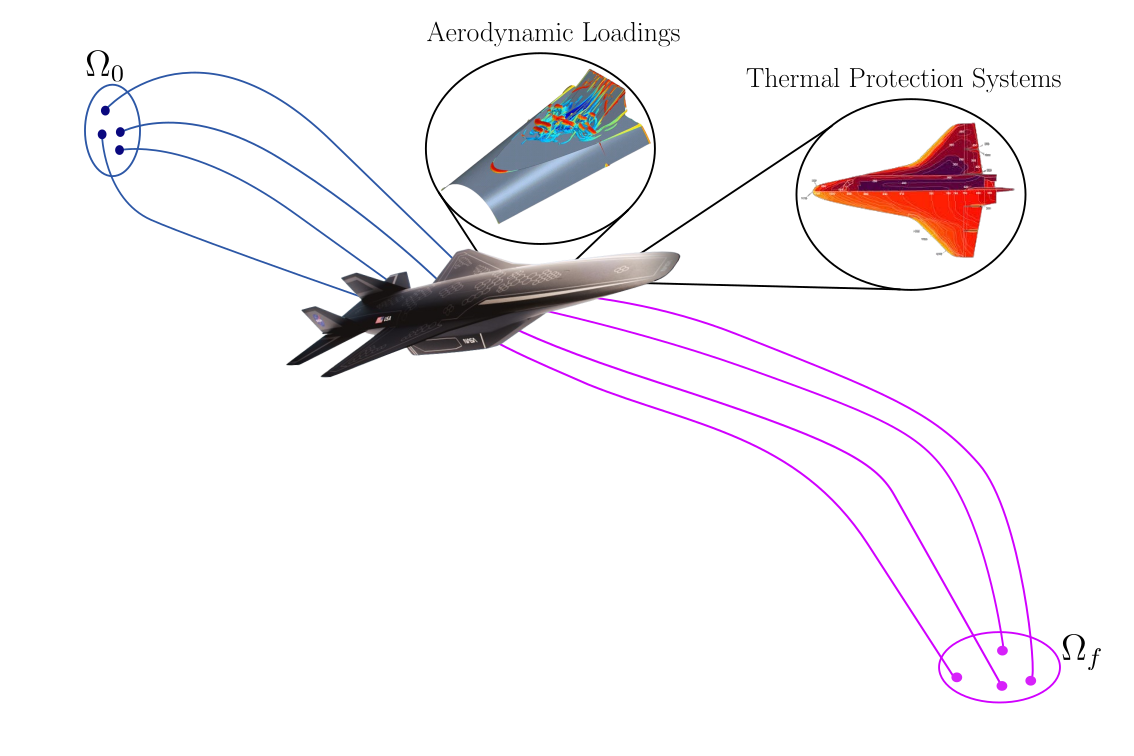
\includegraphics[width=0.9\textwidth]{../figs/introduction/motivating_example_3.png}
%                 \end{figure}}
%             \only<4>{
%                 \begin{figure}
%                     \centering
%                     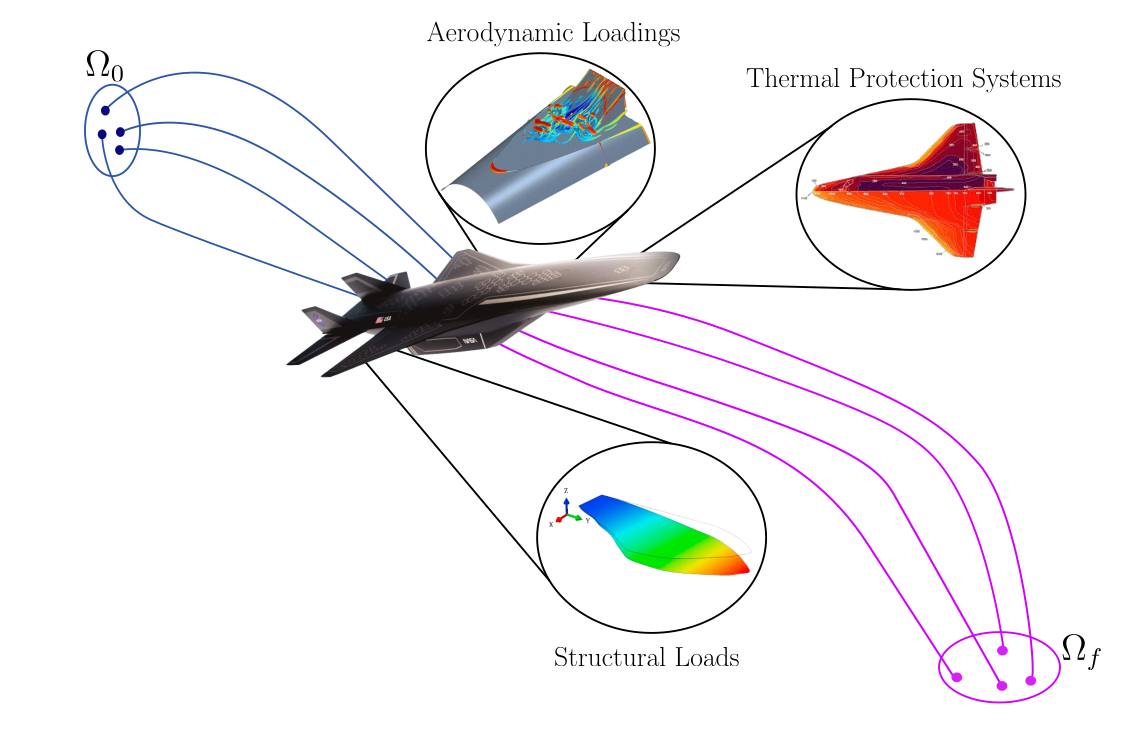
\includegraphics[width=0.9\textwidth]{../figs/introduction/motivating_example_4.png}
%                 \end{figure}}
%             \only<5->{
%                 \begin{figure}
%                     \centering
%                     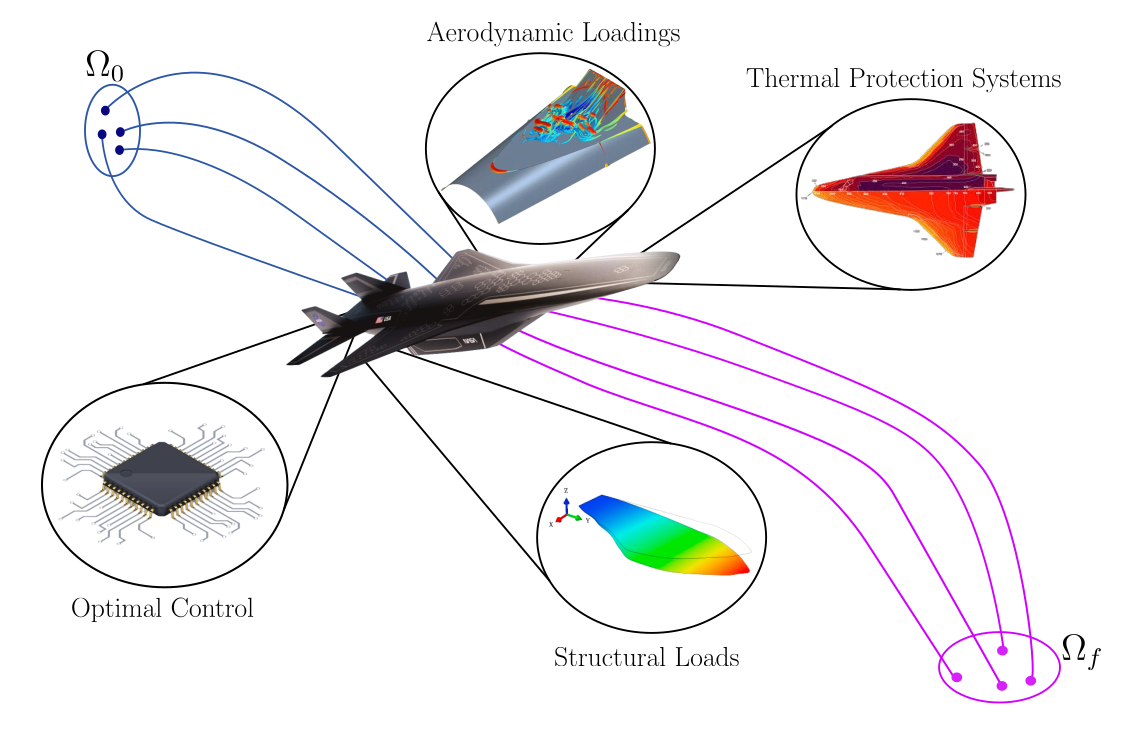
\includegraphics[width=0.9\textwidth]{../figs/introduction/motivating_example_5.png}
%                 \end{figure}}
%         \end{column}
%         \hspace*{-0.4in}
%         \begin{column}{0.45\textwidth}
%             \centering
%             \visible<6->{
%             \begin{graybox}{Simulation}
%                 \visible<7->{
%                 e.g., aero-thermo-servo-elasticity,}
%                 \vspace*{-0.1in}
%                 \begin{align*}
%                     \visible<8->{
%                     \dot{\vu} &= \mathbf{F}\left(\vu;\mathbf{p}\right)}\\
%                     \visible<9->{
%                     \vz_{\text{HF}} &= \mathbf{H}\left(\vu;\vp\right)}\\
%                     \visible<10->{
%                     \vu(t_0) &= \vu_0(\vp)}
%                 \end{align*}
%             \end{graybox}}
%             \visible<11->{
%             \begin{graybox}{Optimal Control/Design}
%                 \visible<12->{
%                 e.g., optimal control problem,}
%                 \vspace*{-0.1in}
%                 \begin{align*}
%                     \visible<13->{
%                     \min_{\vp} \: \mathcal{J} = \int_{t_0}^{t_f} & \ell\left(\vu,\mathbf{p}\right) dt}\\
%                     \visible<14->{
%                     \text{s.t.} \: \quad \dot{\vu} &= \mathbf{F}\left(\vu;\mathbf{p}\right)}\\
%                     \visible<15->{
%                     \mathbf{Q} &\geq \mathbf{g}\left(\vu(t),t;\mathbf{p}\right)}
%                 \end{align*}
%             \end{graybox}}
%         \end{column}
%     \end{columns}
%     \visible<6->{
%     \begin{center}
%         {\tiny
%         $\vu$: high-dimensional states, $\vF$: non-linear dynamics $\vp$: design/control parameters, $\vz_{\text{HF}}$: high-fidelity outputs, $\mathcal{J}$: cost functional, $l$: running cost, $\mathbf{Q}$: safety bound, $\vg$: constraint function}
%     \end{center}}
% \end{frame}

\begin{frame}{\large Motivation: Simulate and Optimally Control Hypersonic Systems}
    \footnotesize
    \only<2>{
        \begin{figure}
            \centering
            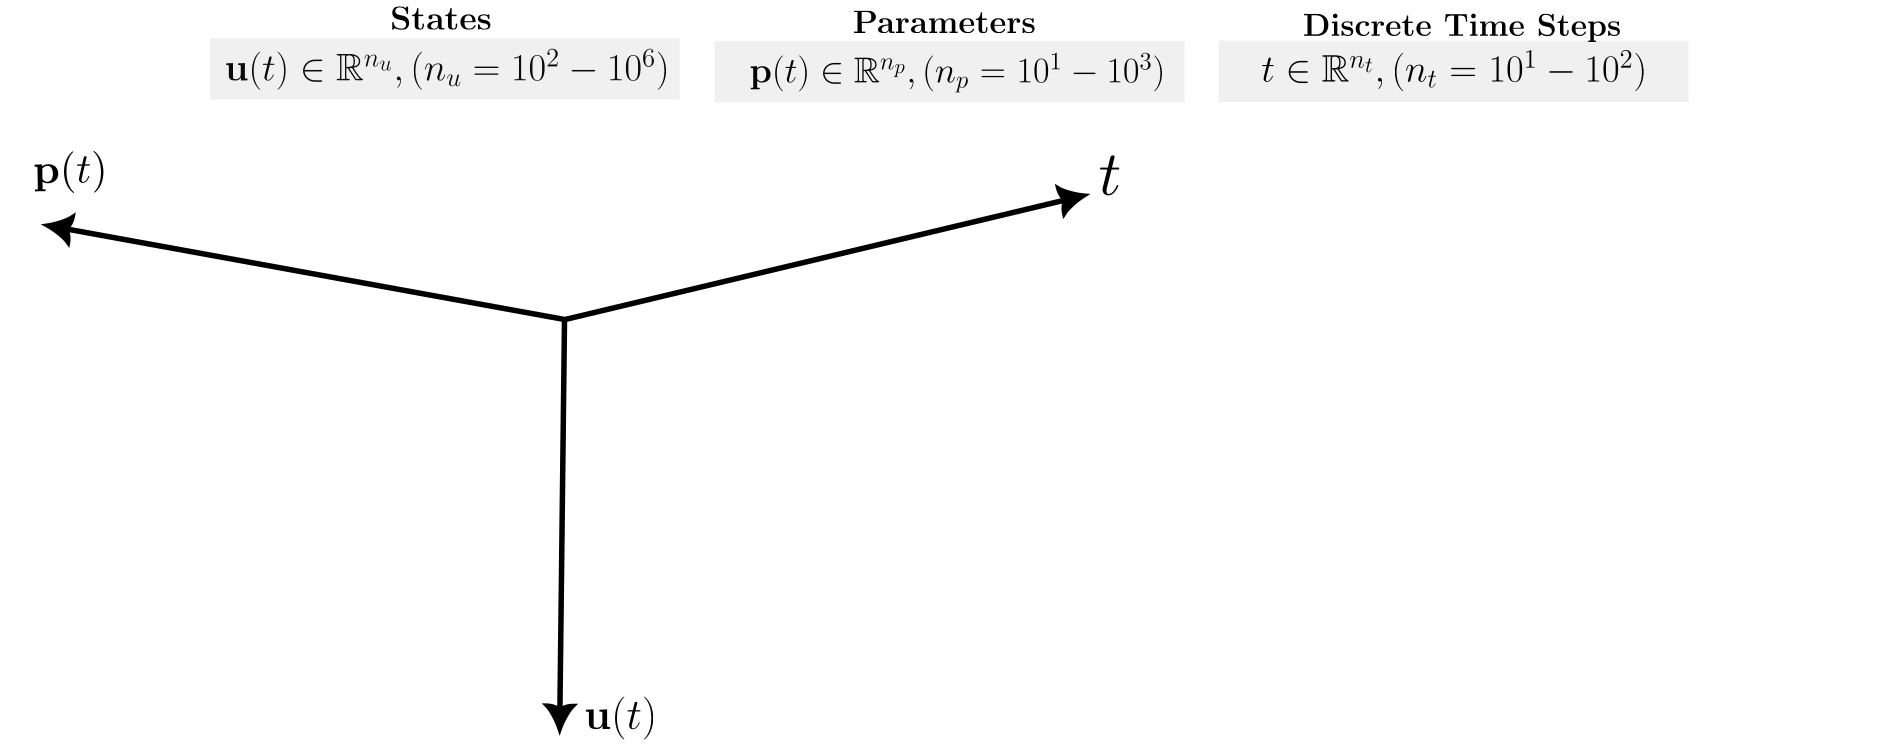
\includegraphics[width=0.95\textwidth]{../figs/introduction/problem_space_1.png}
        \end{figure}}
    \only<3>{
        \begin{figure}
            \centering
            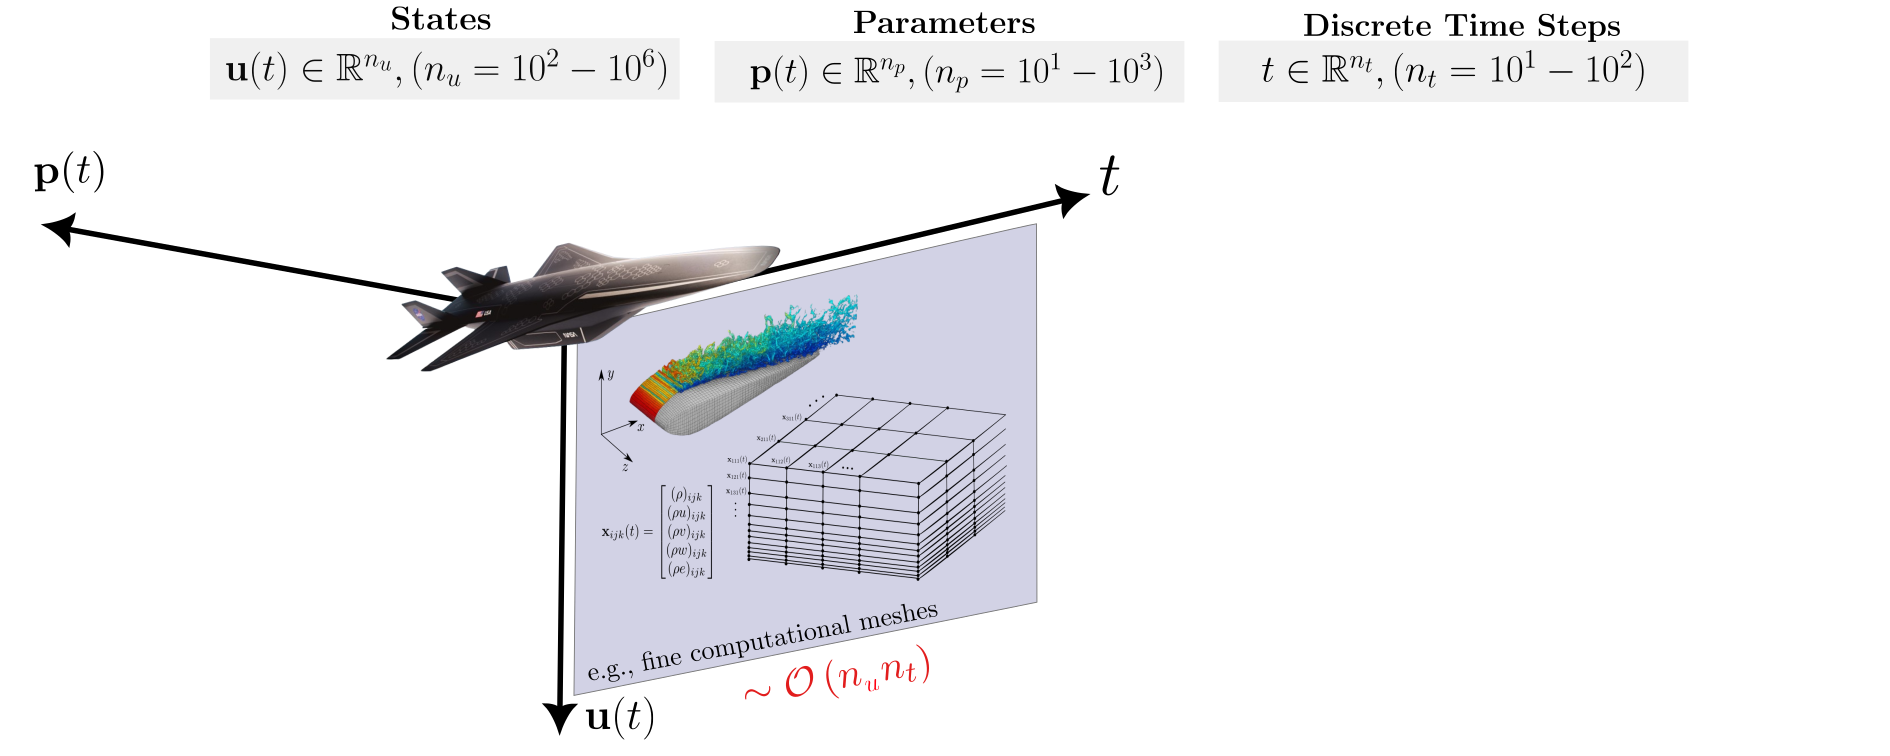
\includegraphics[width=0.95\textwidth]{../figs/introduction/problem_space_2.png}
        \end{figure}}
    \only<4>{
        \begin{figure}
            \centering
            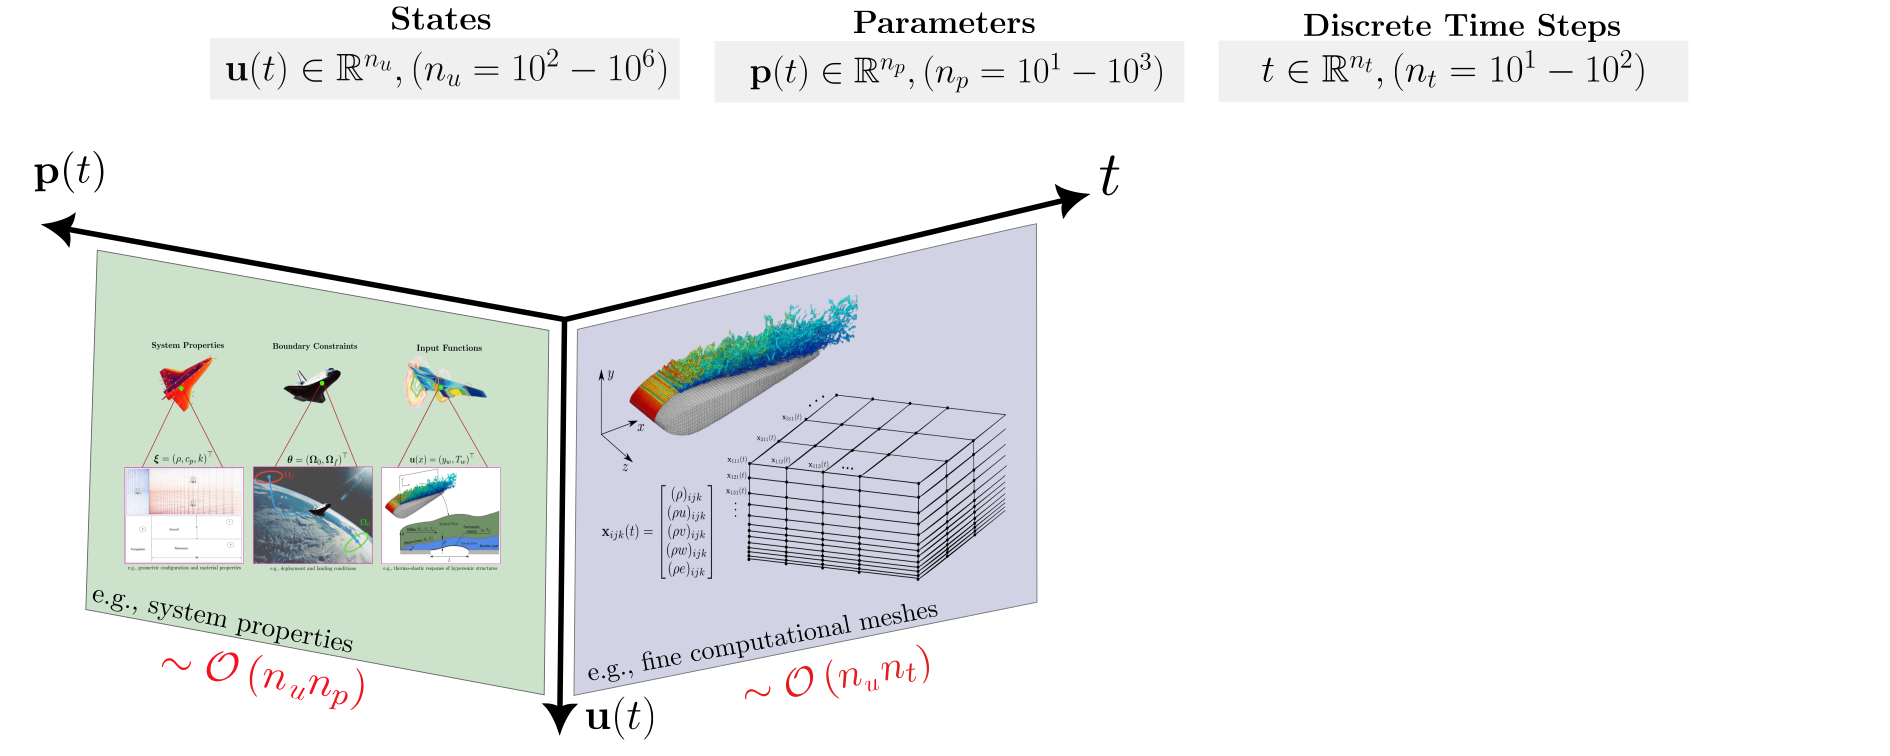
\includegraphics[width=0.95\textwidth]{../figs/introduction/problem_space_3.png}
        \end{figure}}
    \only<5>{
        \begin{figure}
            \centering
            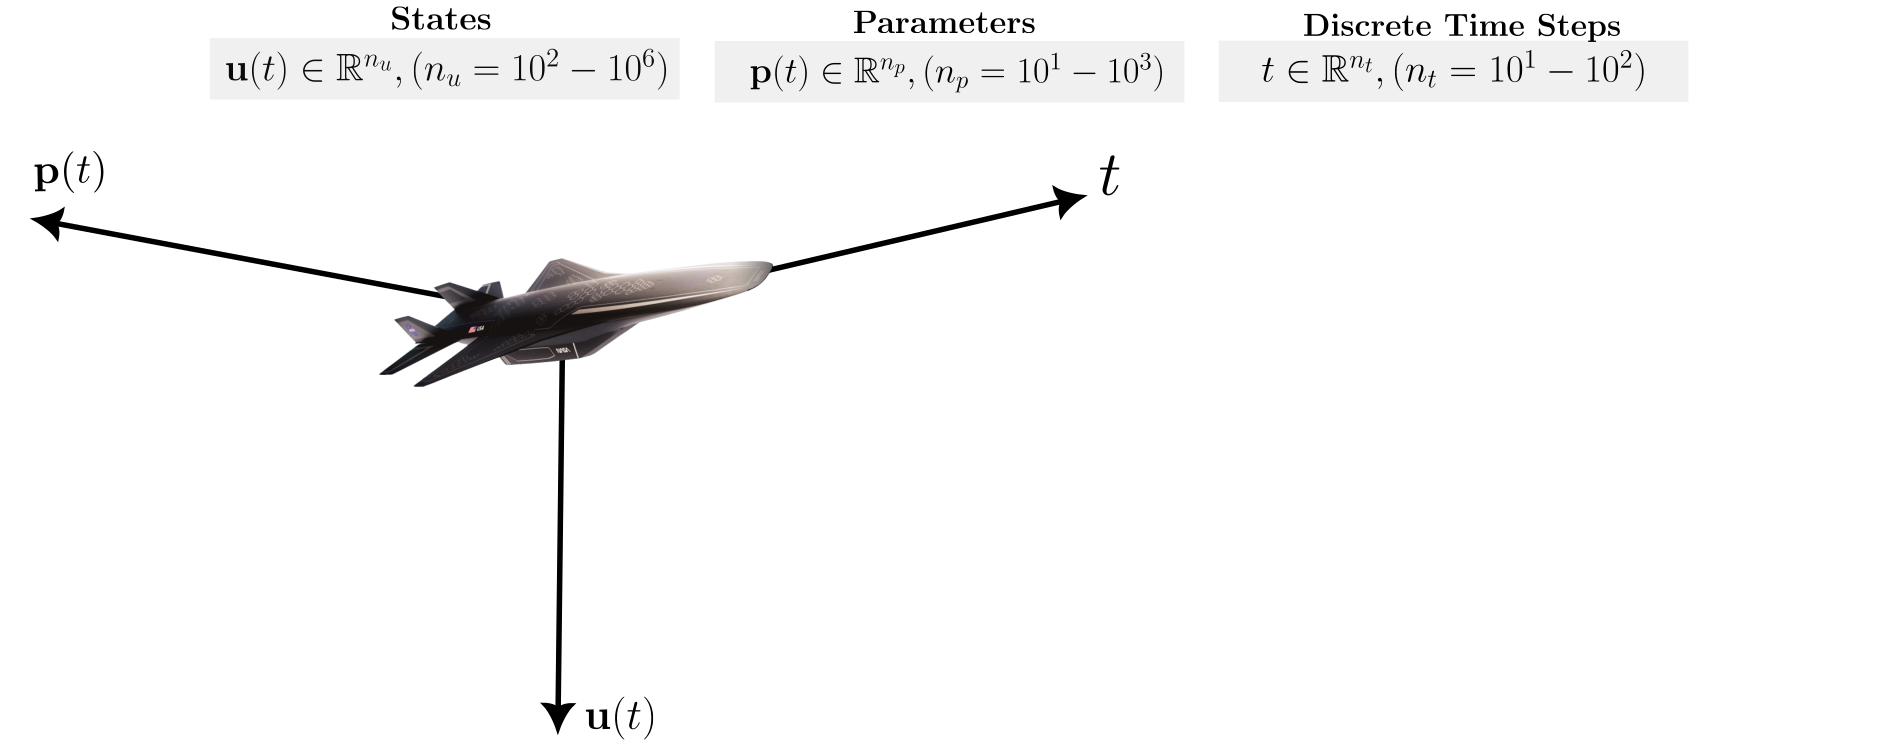
\includegraphics[width=0.95\textwidth]{../figs/introduction/problem_space_4.png}
        \end{figure}}
    \only<6>{
        \begin{figure}
            \centering
            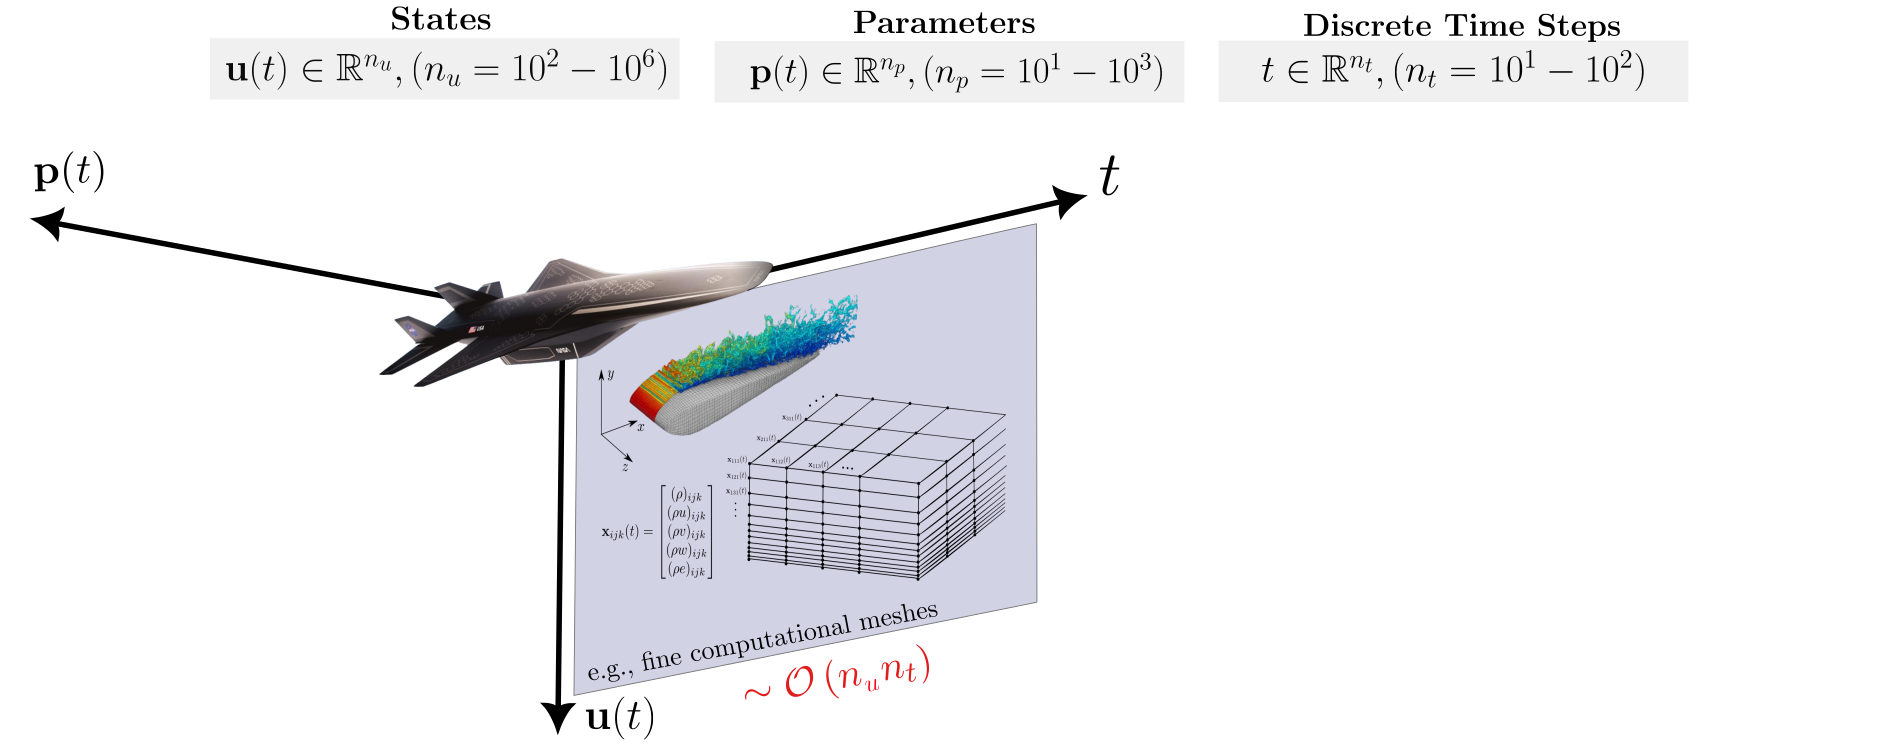
\includegraphics[width=0.95\textwidth]{../figs/introduction/problem_space_5.png}
        \end{figure}}
    \only<7>{
        \begin{figure}
            \centering
            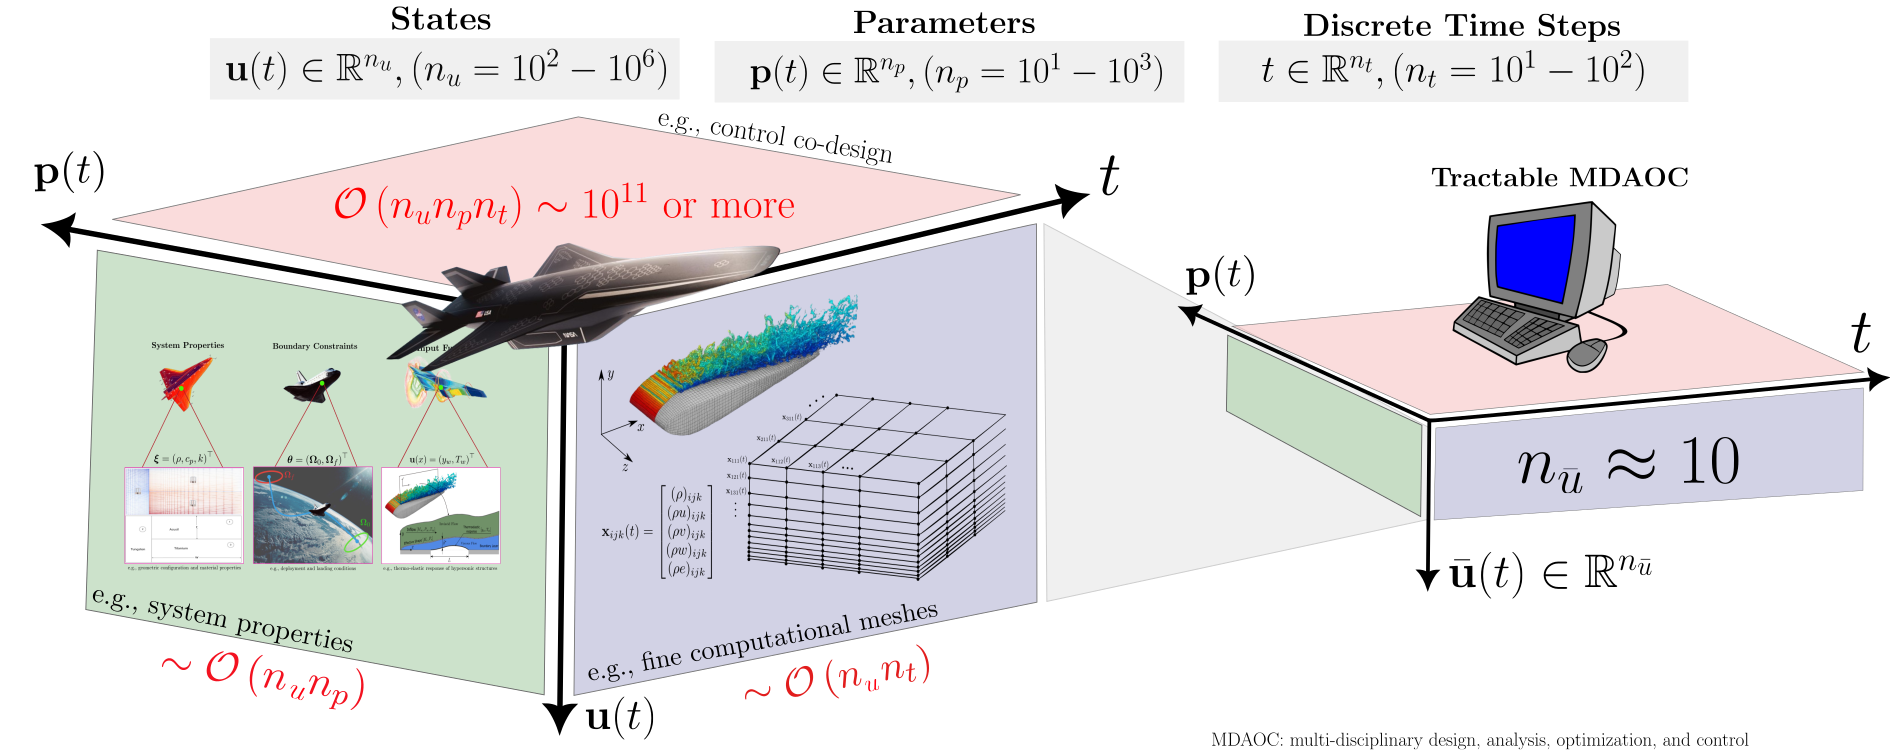
\includegraphics[width=0.95\textwidth]{../figs/introduction/problem_space_6.png}
        \end{figure}}
    \only<8->{
        \begin{figure}
            \centering
            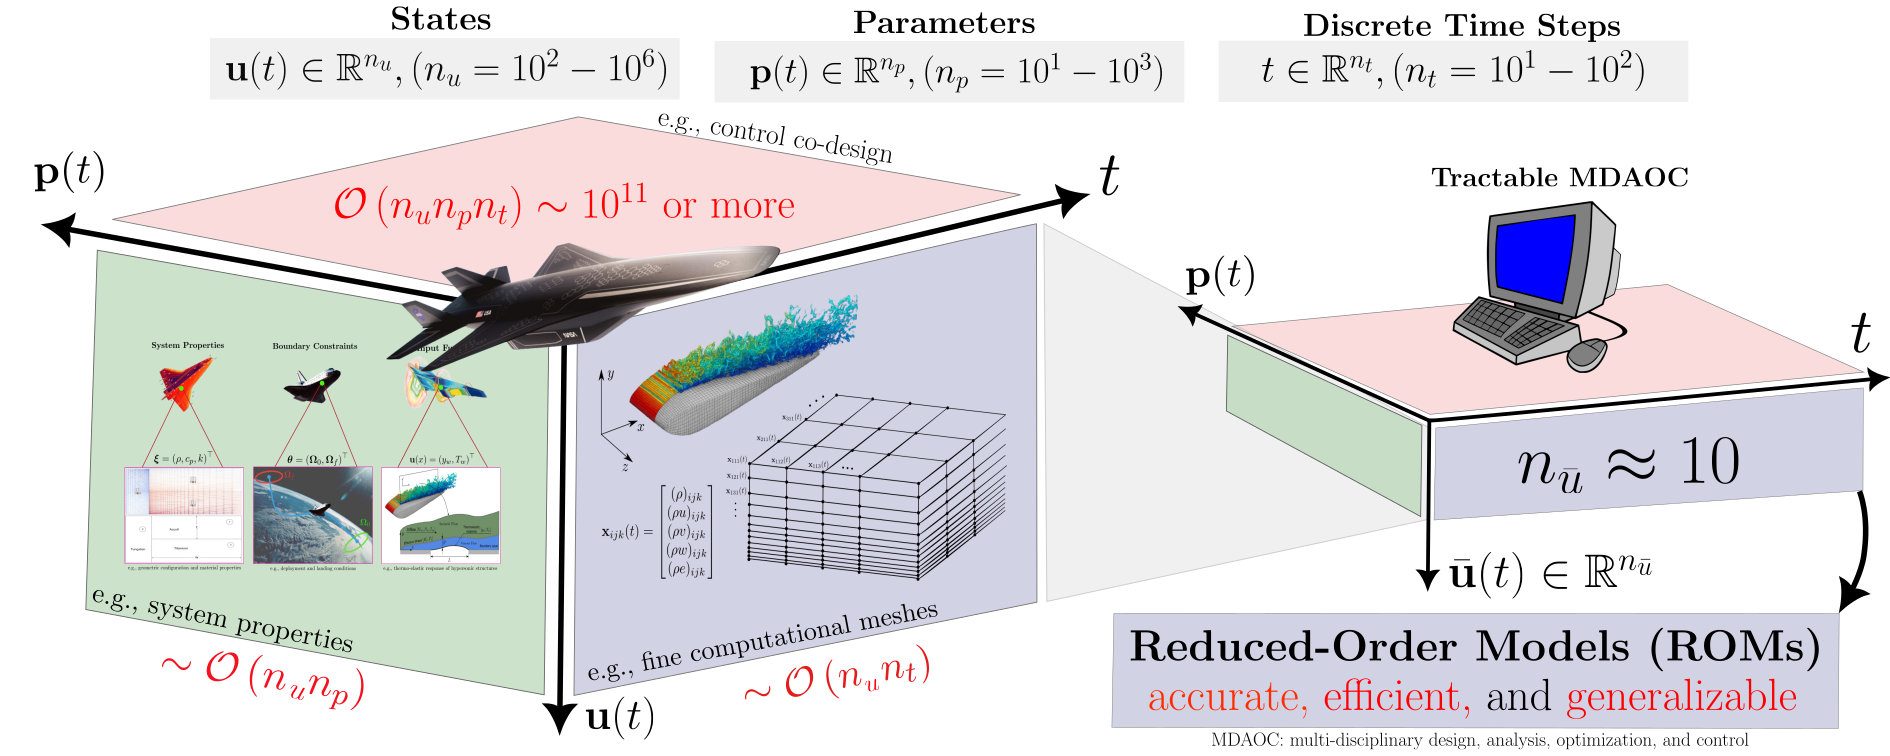
\includegraphics[width=0.95\textwidth]{../figs/introduction/problem_space_7.png}
        \end{figure}}
\end{frame}

\begin{frame}{\large ITM in Simulation: Balancing Accuracy, Efficiency, and Generalizability with Little Data}
    \footnotesize
    \hspace*{-0.1in}
    \begin{columns}
        \begin{column}{0.65\textwidth}
            \only<1-2>{
                \begin{figure}
                    \centering
                    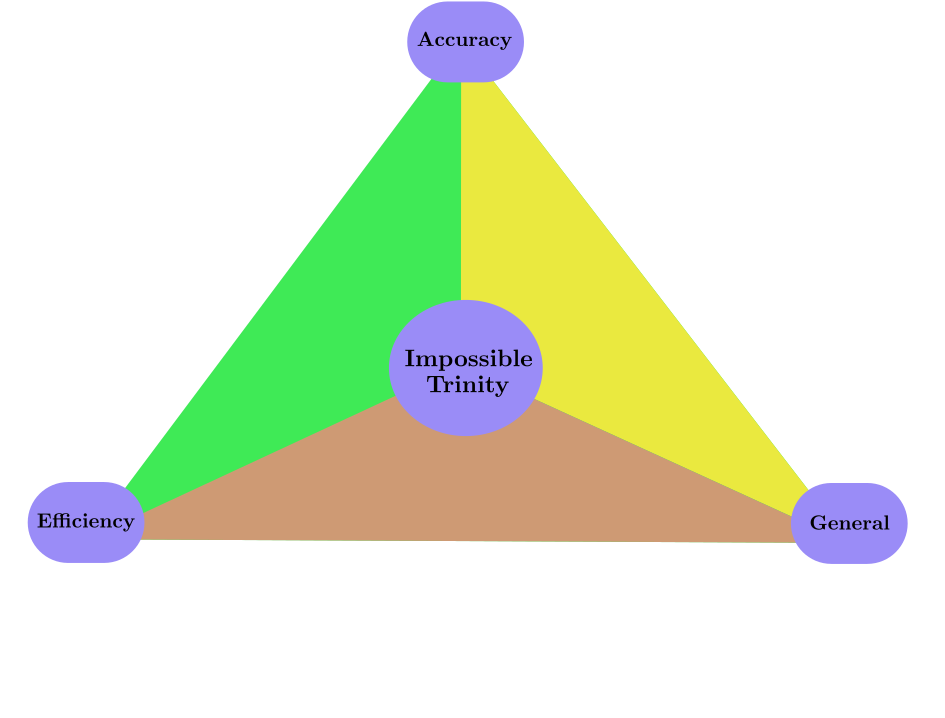
\includegraphics[width=0.8\textwidth]{../figs/introduction/itm_1.png}
                \end{figure}}
            \only<3>{
                \begin{figure}
                    \centering
                    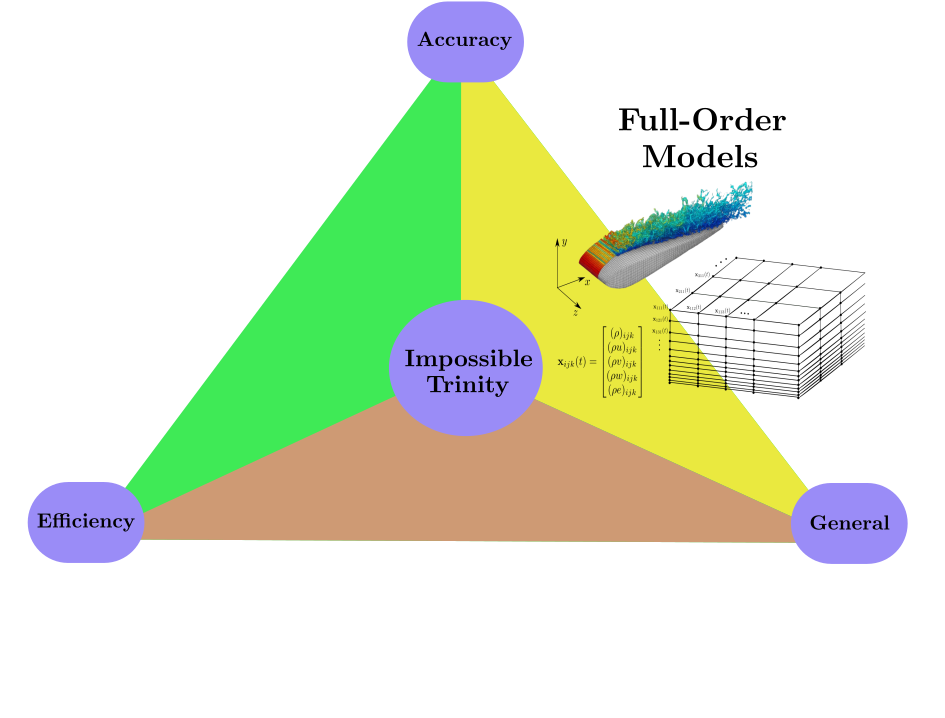
\includegraphics[width=0.8\textwidth]{../figs/introduction/itm_2.png}
                \end{figure}}
            \only<4>{
                \begin{figure}
                    \centering
                    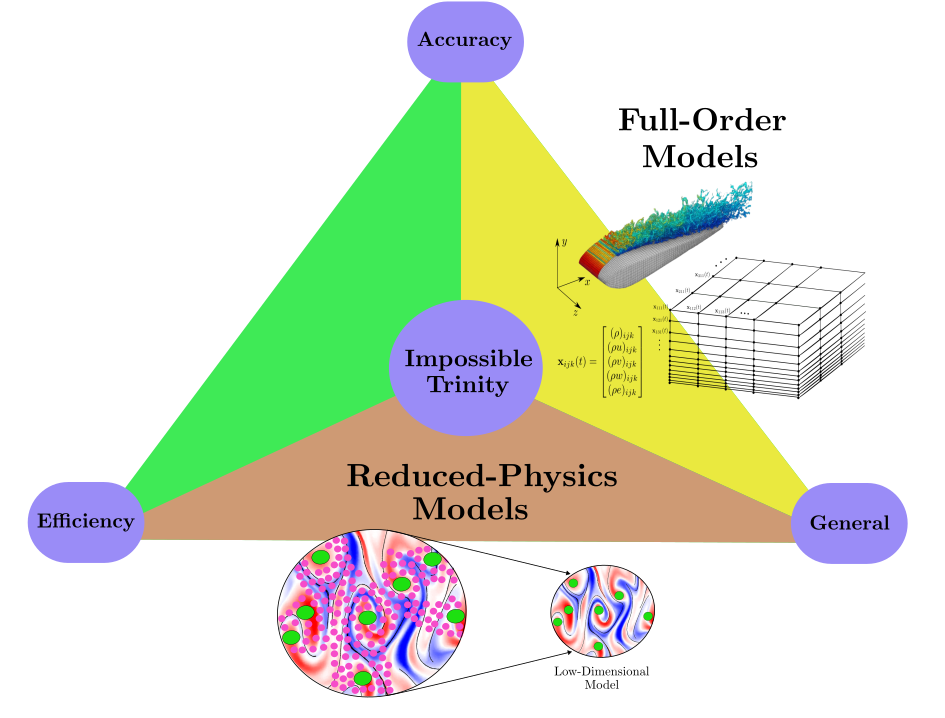
\includegraphics[width=0.8\textwidth]{../figs/introduction/itm_3.png}
                \end{figure}}
            \only<5->{
                \begin{figure}
                    \centering
                    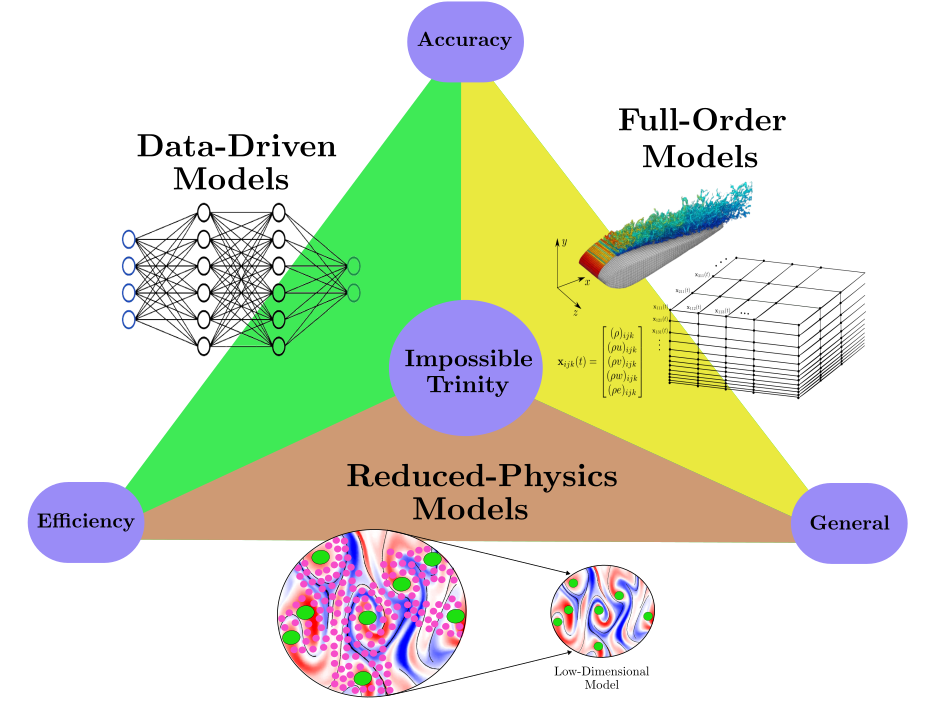
\includegraphics[width=0.8\textwidth]{../figs/introduction/itm_4.png}
                \end{figure}}
        \end{column}
        \hspace*{-0.3in}
        \begin{column}{0.46\textwidth}
            \visible<2->{
            \noindent Remains largely \textbf{unresolved} because,}
            \begin{itemize}
                \item<3-> \textbf{FEMs}: too many states,
                \item<4-> \textbf{RPMs}: overly simplified problems,
                \item<5-> \textbf{NNs}: need too much data,
            \end{itemize}
        \end{column}
    \end{columns}
    \begin{center}
        \vspace*{-0.2in}
        {\tiny ITM: Impossible Trinity of Modeling, FEM: finite-element method, RPM: reduced-physics model, NN: neural network}
    \end{center}
\end{frame}

\begin{frame}{\large ITOC: Balancing Accuracy, Efficiency, and Generalizability With Little Data}
    \footnotesize
    \begin{columns}
        \begin{column}{0.65\textwidth}
            \only<1-2>{
                \begin{figure}
                    \centering
                    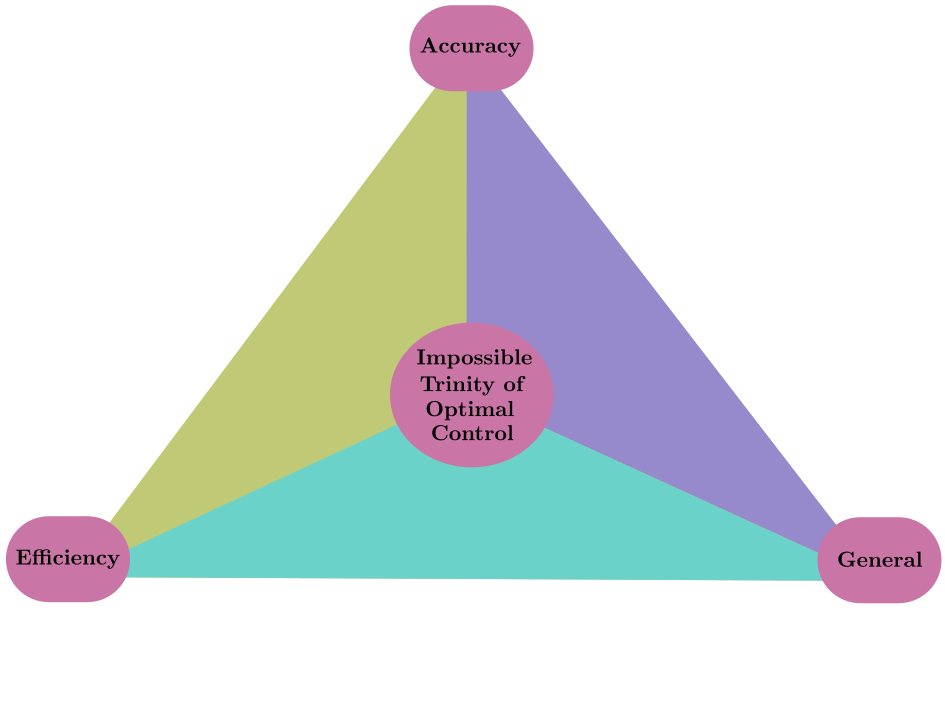
\includegraphics[width=0.8\textwidth]{../figs/introduction/itoc_1.png}
                \end{figure}}
            \only<3>{
                \begin{figure}
                    \centering
                    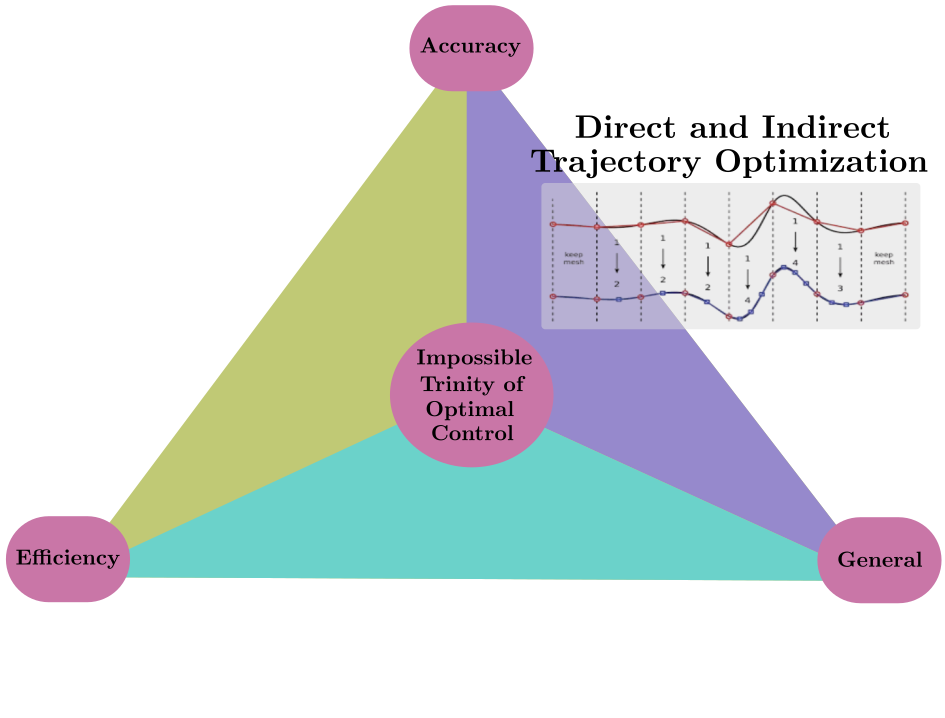
\includegraphics[width=0.8\textwidth]{../figs/introduction/itoc_2.png}
                \end{figure}}
            \only<4>{
                \begin{figure}
                    \centering
                    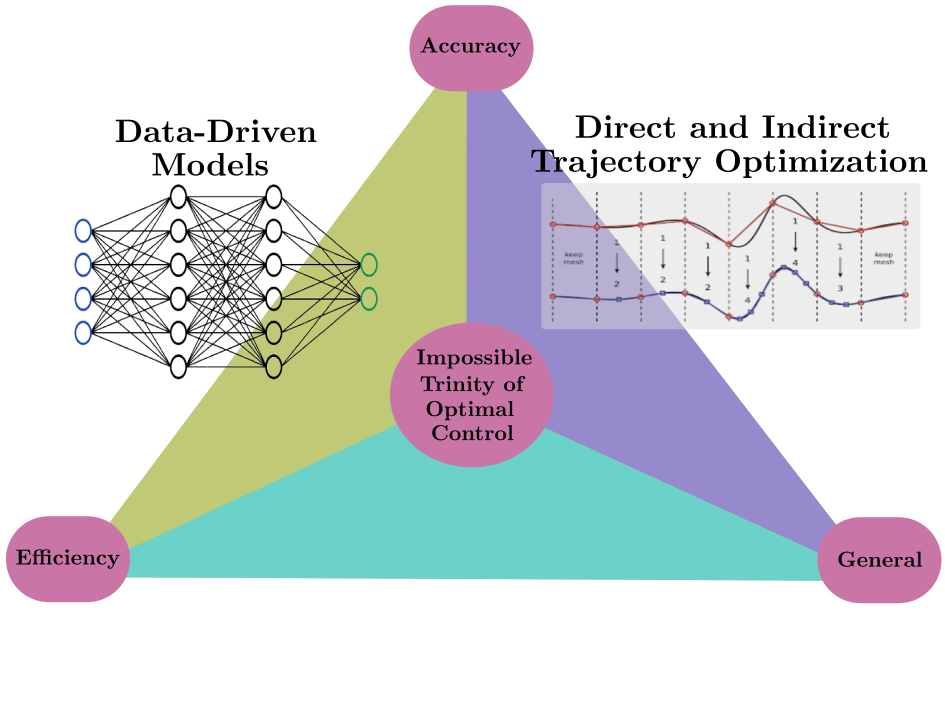
\includegraphics[width=0.8\textwidth]{../figs/introduction/itoc_3.png}
                \end{figure}}
            \only<5->{
                \begin{figure}
                    \centering
                    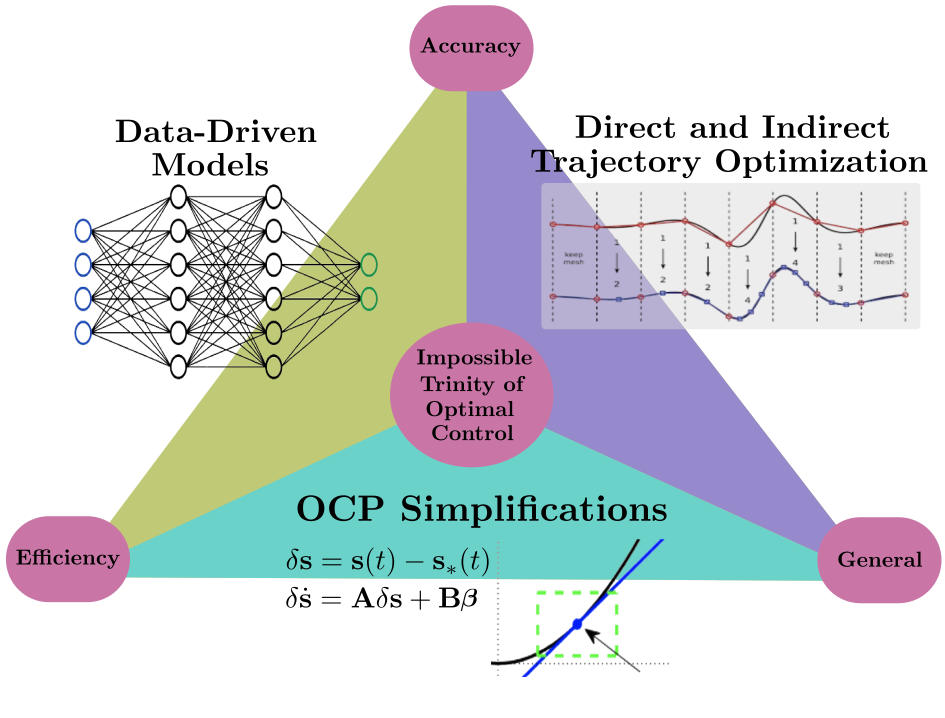
\includegraphics[width=0.8\textwidth]{../figs/introduction/itoc_4.png}
                \end{figure}}
        \end{column}
        \hspace*{-0.2in}
        \begin{column}{0.5\textwidth}
            \visible<2->{
            \noindent Remains largely \textbf{unresolved} because,}
            \begin{itemize}
                \item<3-> \textbf{TO}: need discretization and optimization,
                \item<4-> \textbf{NNs}: scarce data,
                \item<5-> \textbf{Linearizations}: not the original problem
            \end{itemize}
        \end{column}
    \end{columns}
    \visible<1->{
    \begin{center}
        {\tiny ITOC: Impossible Trinity of Optimal Control, TO: trajectory optimization, OCP: optimal control problem}
    \end{center}}
\end{frame}

\begin{frame}{\large Objectives of Research}
    \footnotesize
    \vspace*{0.1in}
    \only<1>{
        \begin{figure}
            \centering
            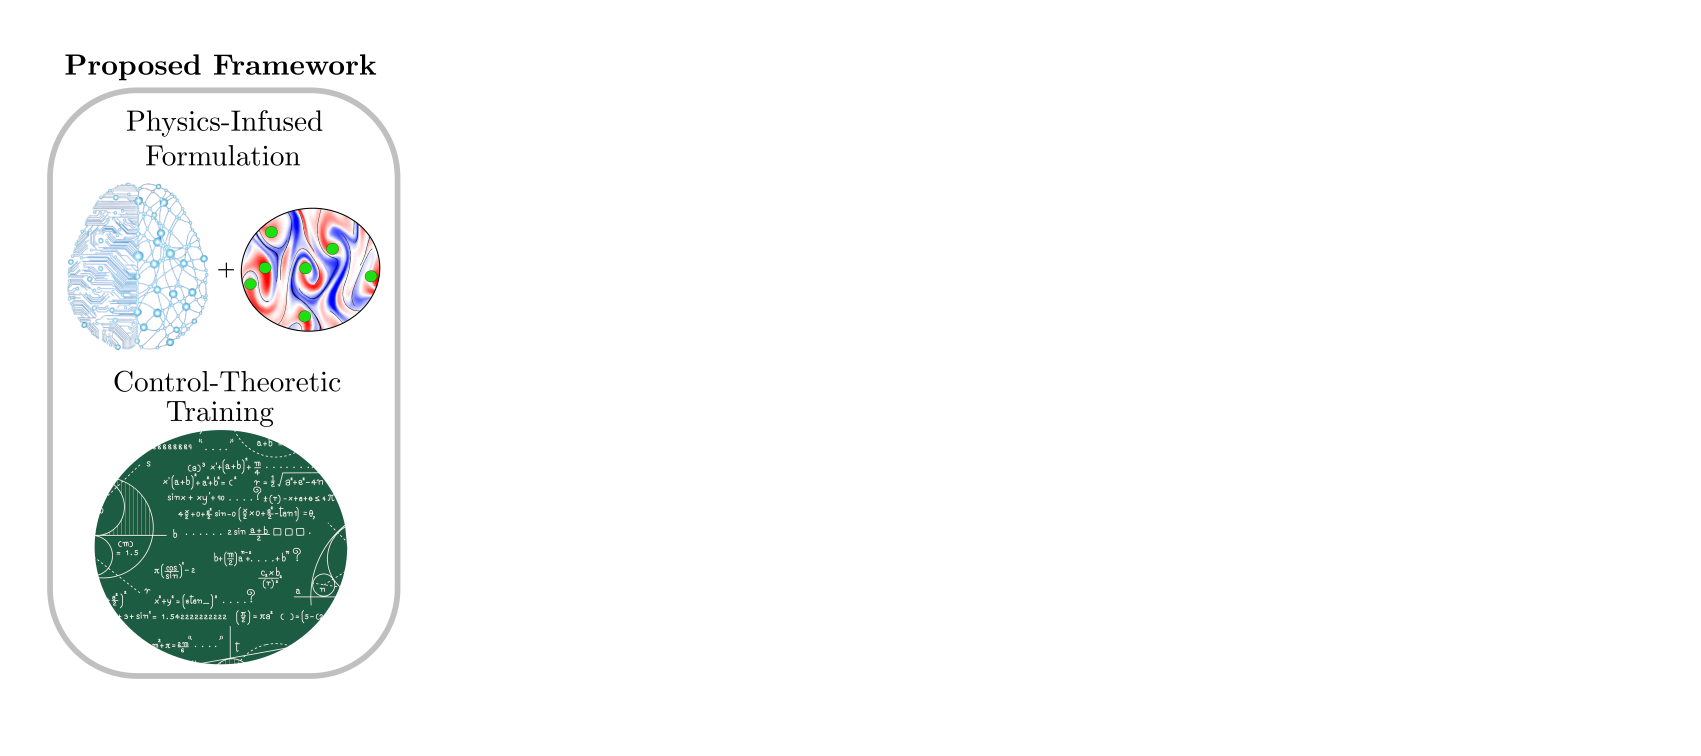
\includegraphics[width=1.0\textwidth]{../figs/introduction/objectives_1.png}
        \end{figure}}
    \only<2>{
        \begin{figure}
            \vspace*{-0.1in}
            \centering
            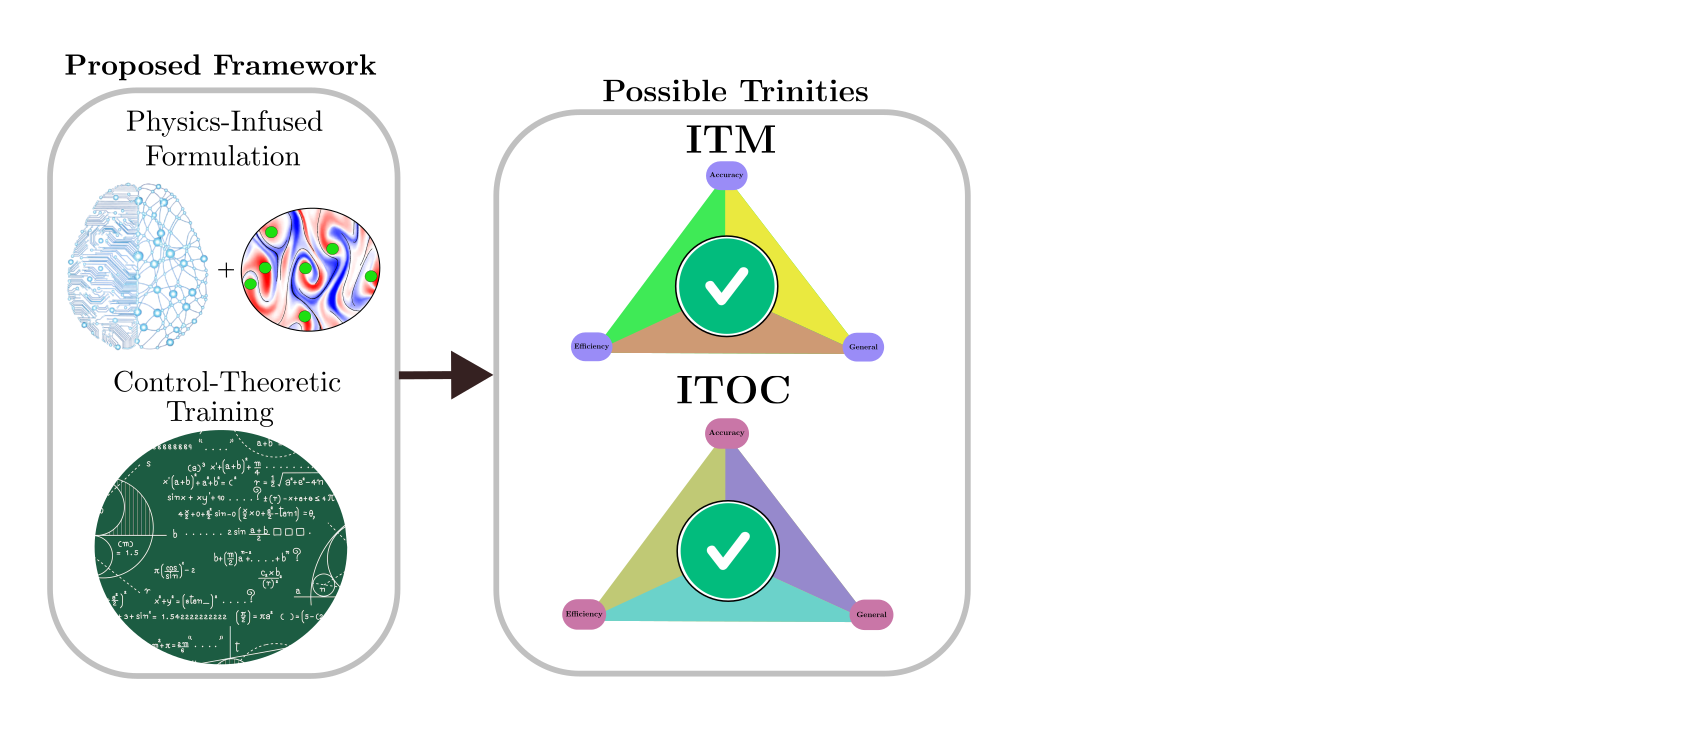
\includegraphics[width=1.0\textwidth]{../figs/introduction/objectives_2.png}
        \end{figure}}
    \only<3->{
        \begin{figure}
            \vspace*{-0.1in}
            \centering
            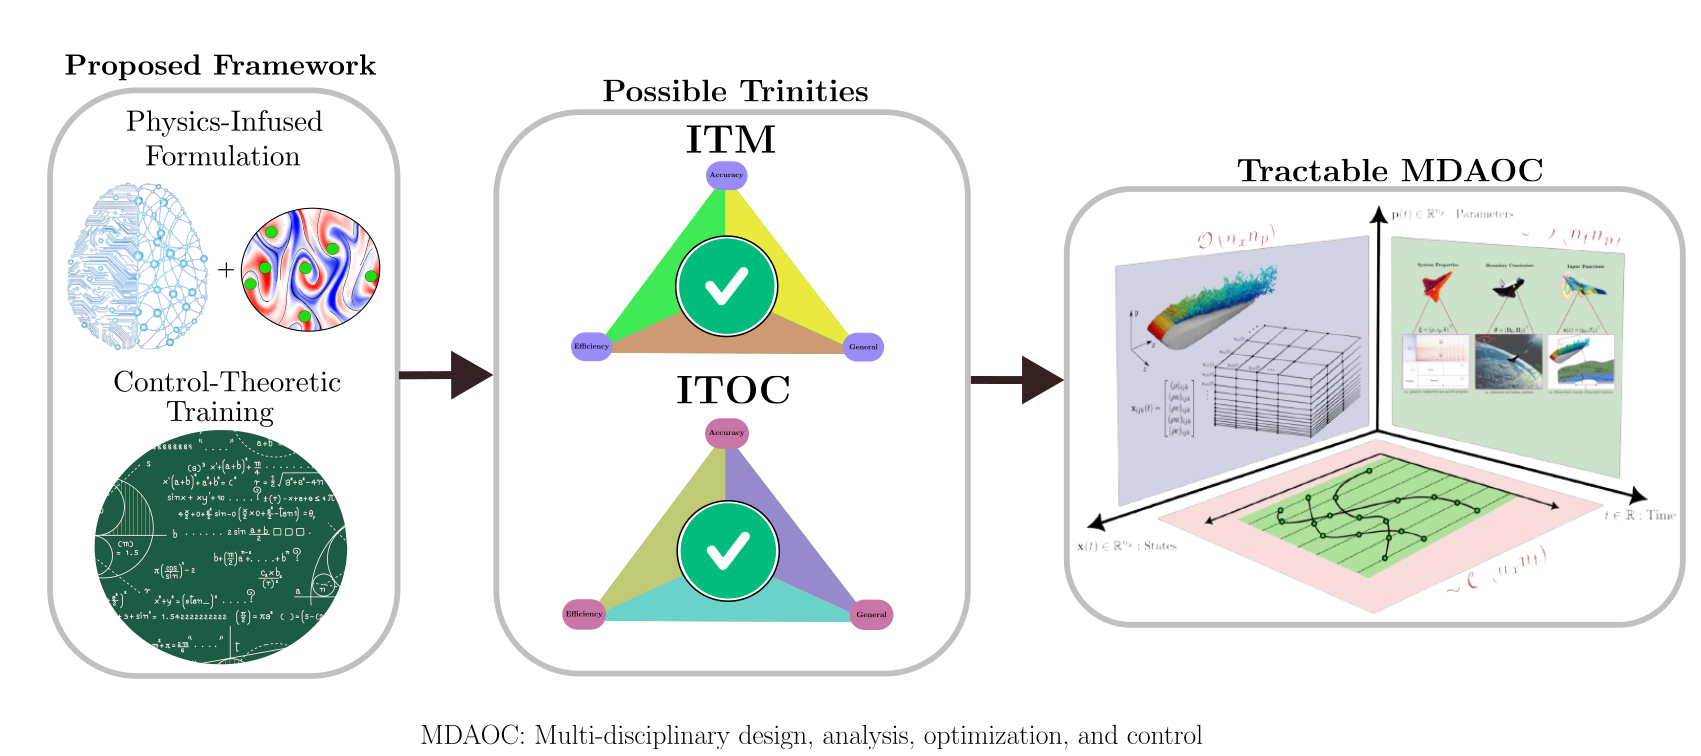
\includegraphics[width=1.0\textwidth]{../figs/introduction/objectives_3.png}
        \end{figure}}
\end{frame}


% part 2: itm
\begin{frame}{Content Overview}
  \footnotesize
    \begin{enumerate}
        \item \textcolor{gray!50}{Motivation, Background, and Objectives}
        \item \colorbox{yellow!70}{\textbf{Addressing the Impossible Trinity of Modeling (ITM)}}
        \item \textcolor{gray!50}{Unified Control-Theoretic Training}
        \item \textcolor{gray!50}{Addressing the Impossible Trinity of Optimal Control (ITOC)}
        \item \textcolor{gray!50}{Conclusions and Future Work}
    \end{enumerate}
\end{frame}

\begin{frame}{\large How does PIROM solve the ITM in small-data regimes?}
    \footnotesize
    \only<1>{
    \begin{figure}
        \centering
        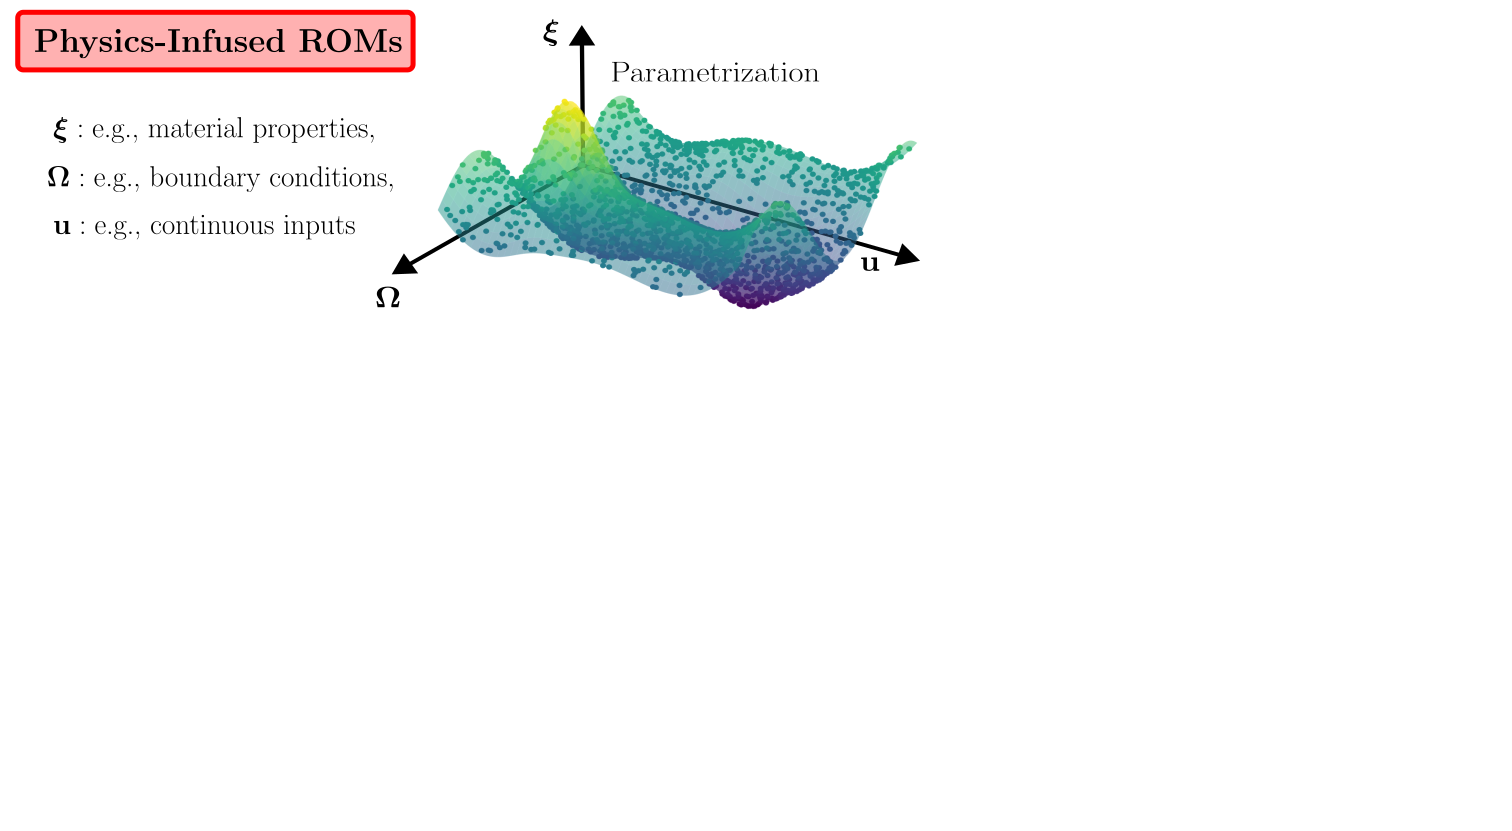
\includegraphics[width=0.9\textwidth]{../figs/sota/physics_infused_1.png}
    \end{figure}}
    \only<2>{
    \begin{figure}
        \centering
        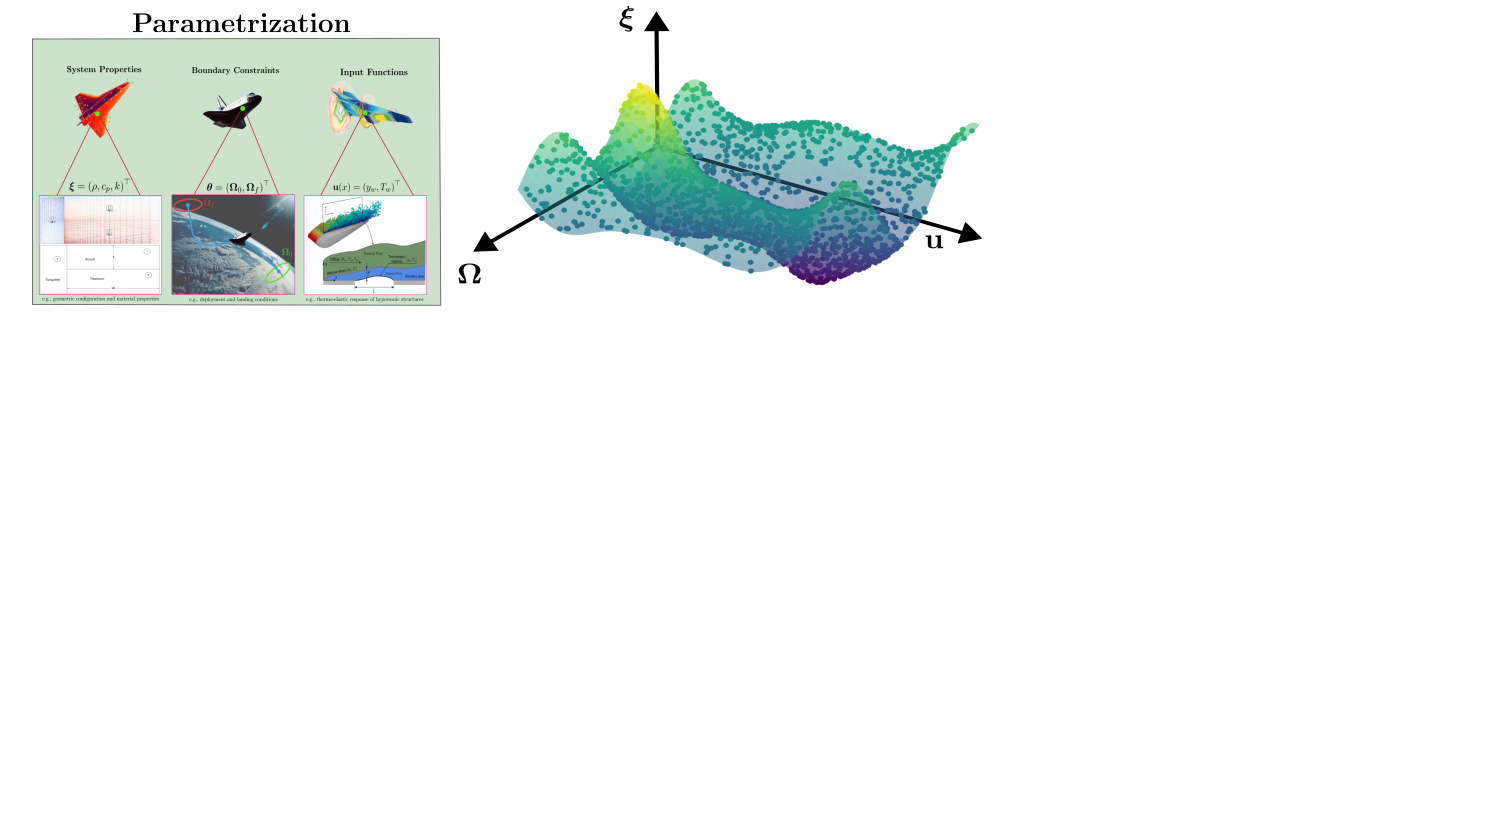
\includegraphics[width=0.9\textwidth]{../figs/sota/physics_infused_2.png}
    \end{figure}}
    \only<3>{
    \begin{figure}
        \centering
        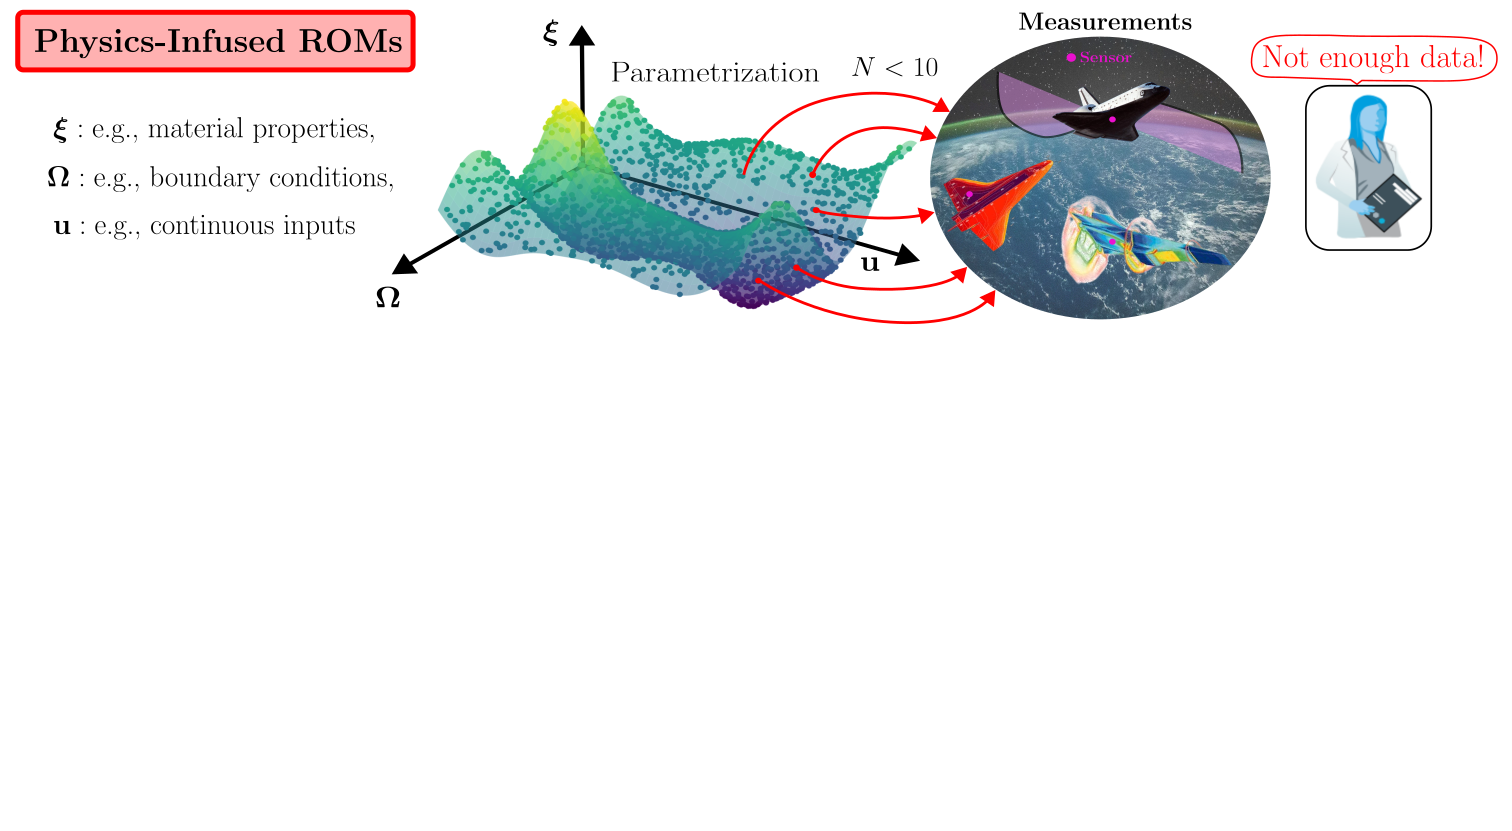
\includegraphics[width=0.9\textwidth]{../figs/sota/physics_infused_3.png}
    \end{figure}}
    \only<4>{
    \begin{figure}
        \centering
        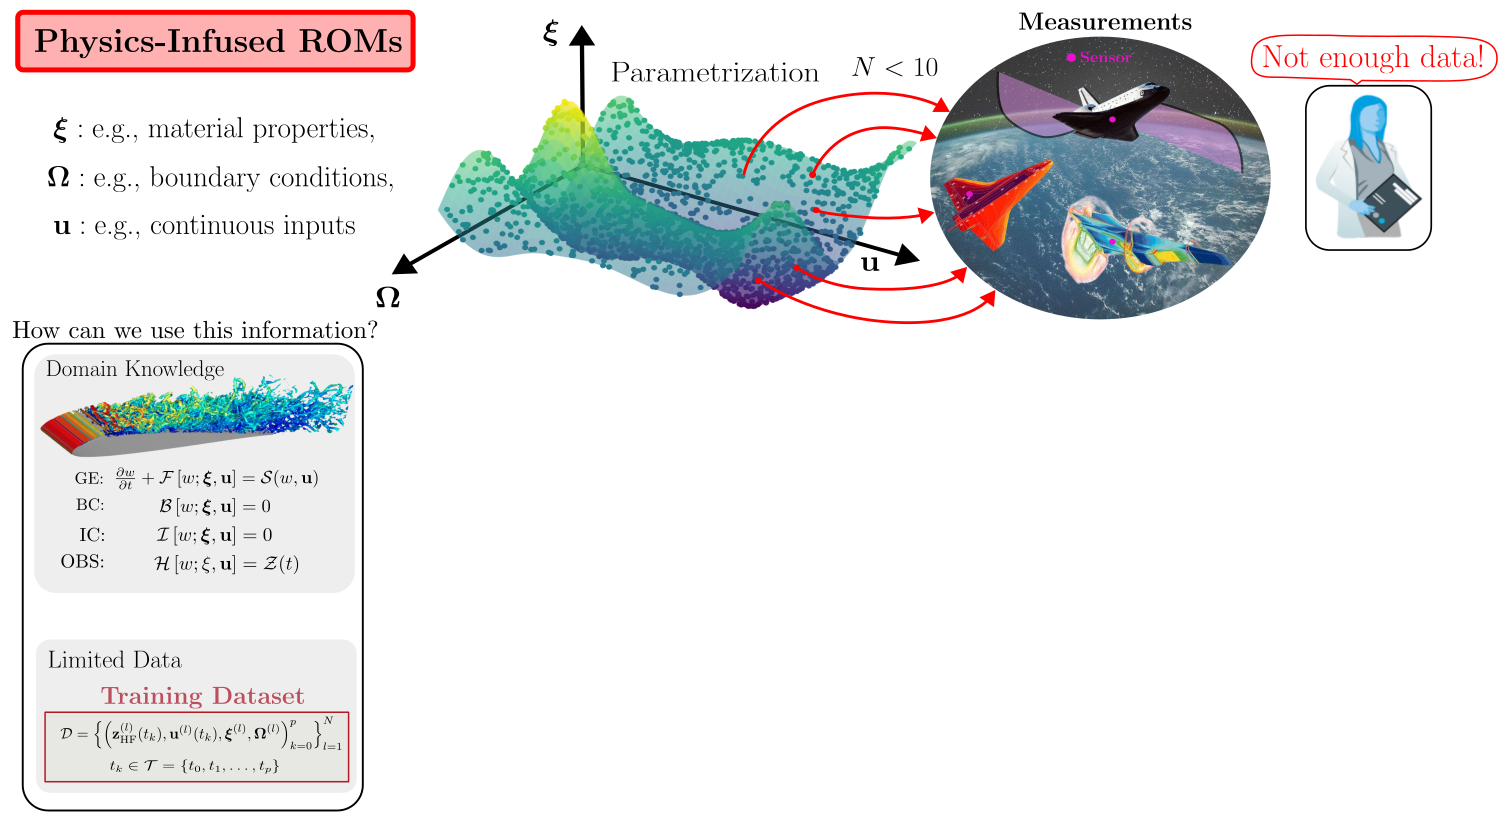
\includegraphics[width=0.9\textwidth]{../figs/sota/physics_infused_4.png}
    \end{figure}}
    \only<5>{
    \begin{figure}
        \centering
        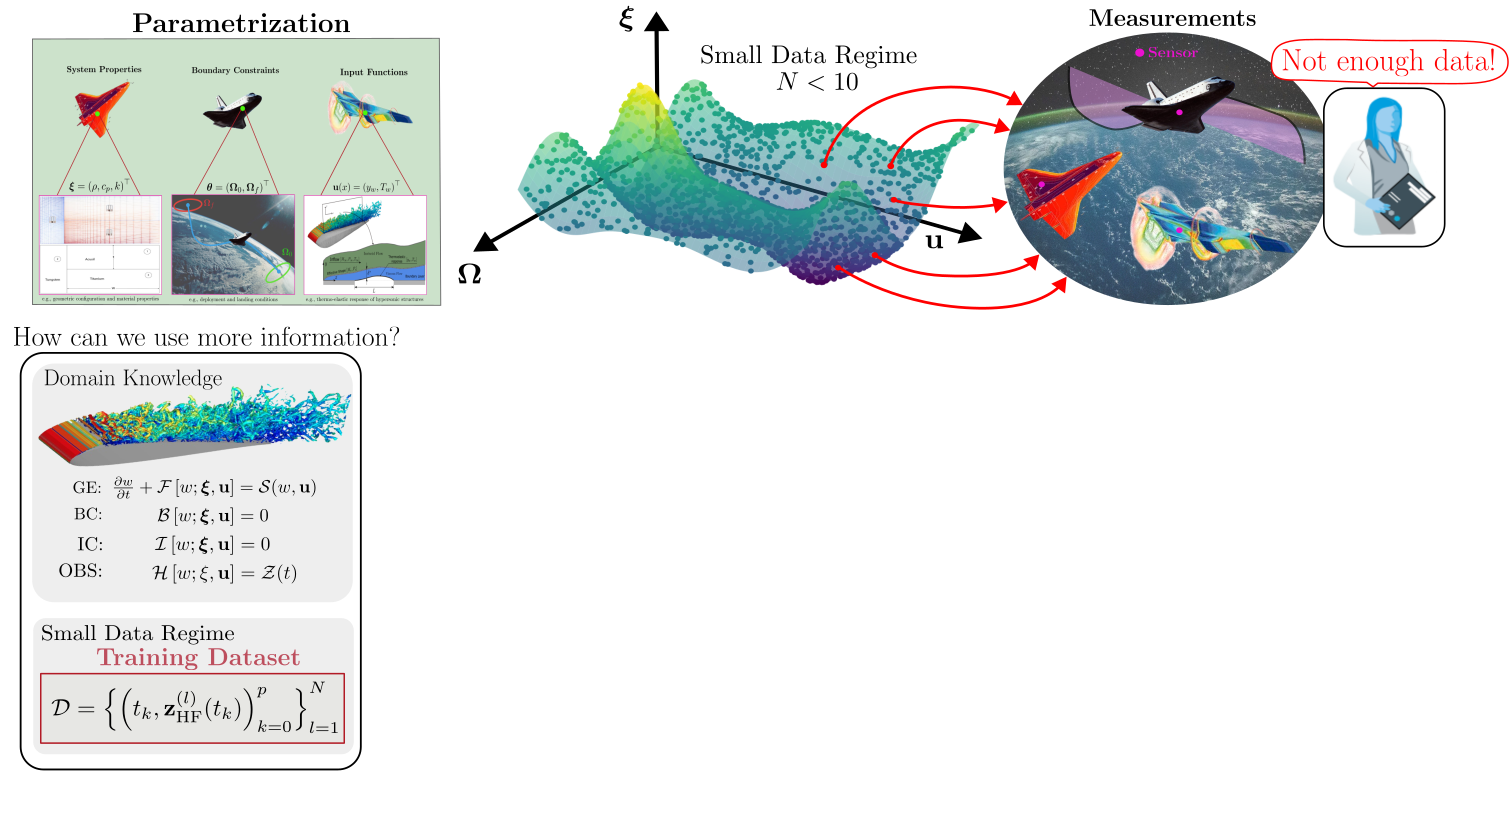
\includegraphics[width=0.9\textwidth]{../figs/sota/physics_infused_5.png}
    \end{figure}}
    \only<6>{
    \begin{figure}
        \centering
        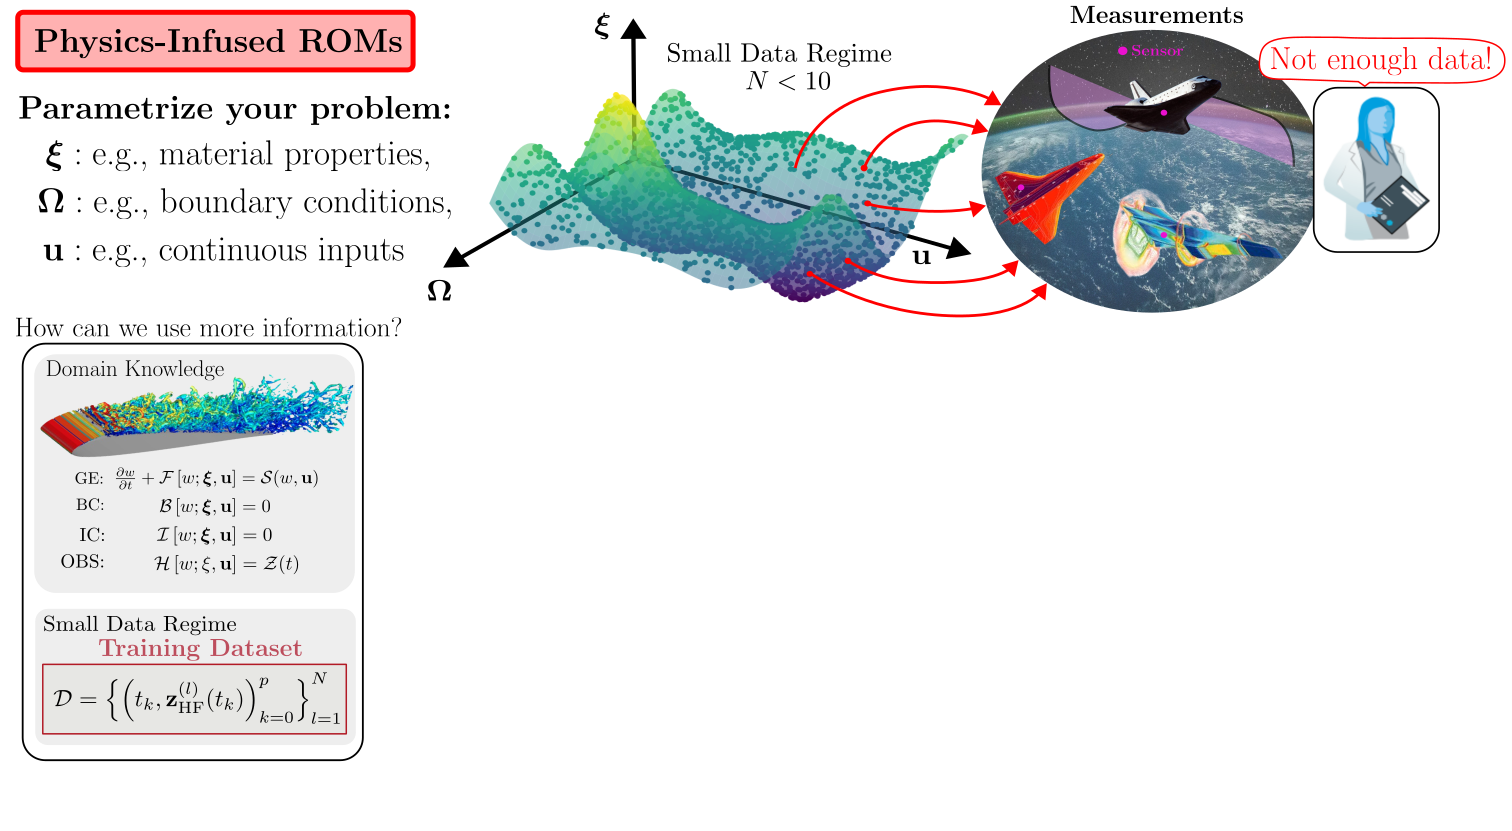
\includegraphics[width=0.9\textwidth]{../figs/sota/physics_infused_6.png}
    \end{figure}}
    \only<7>{
    \begin{figure}
        \centering
        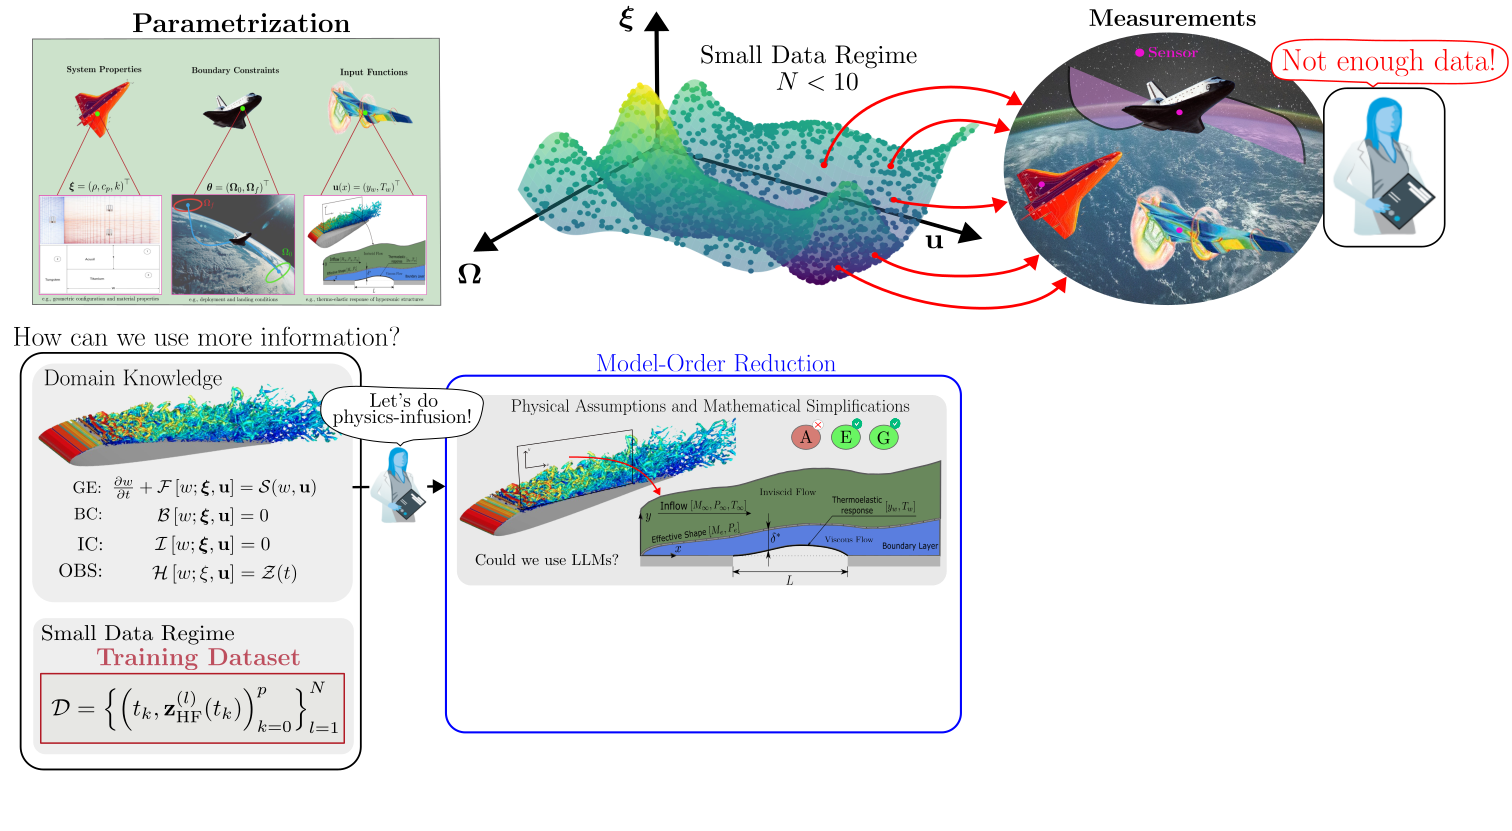
\includegraphics[width=0.9\textwidth]{../figs/sota/physics_infused_7.png}
    \end{figure}}
    \only<8>{
    \begin{figure}
        \centering
        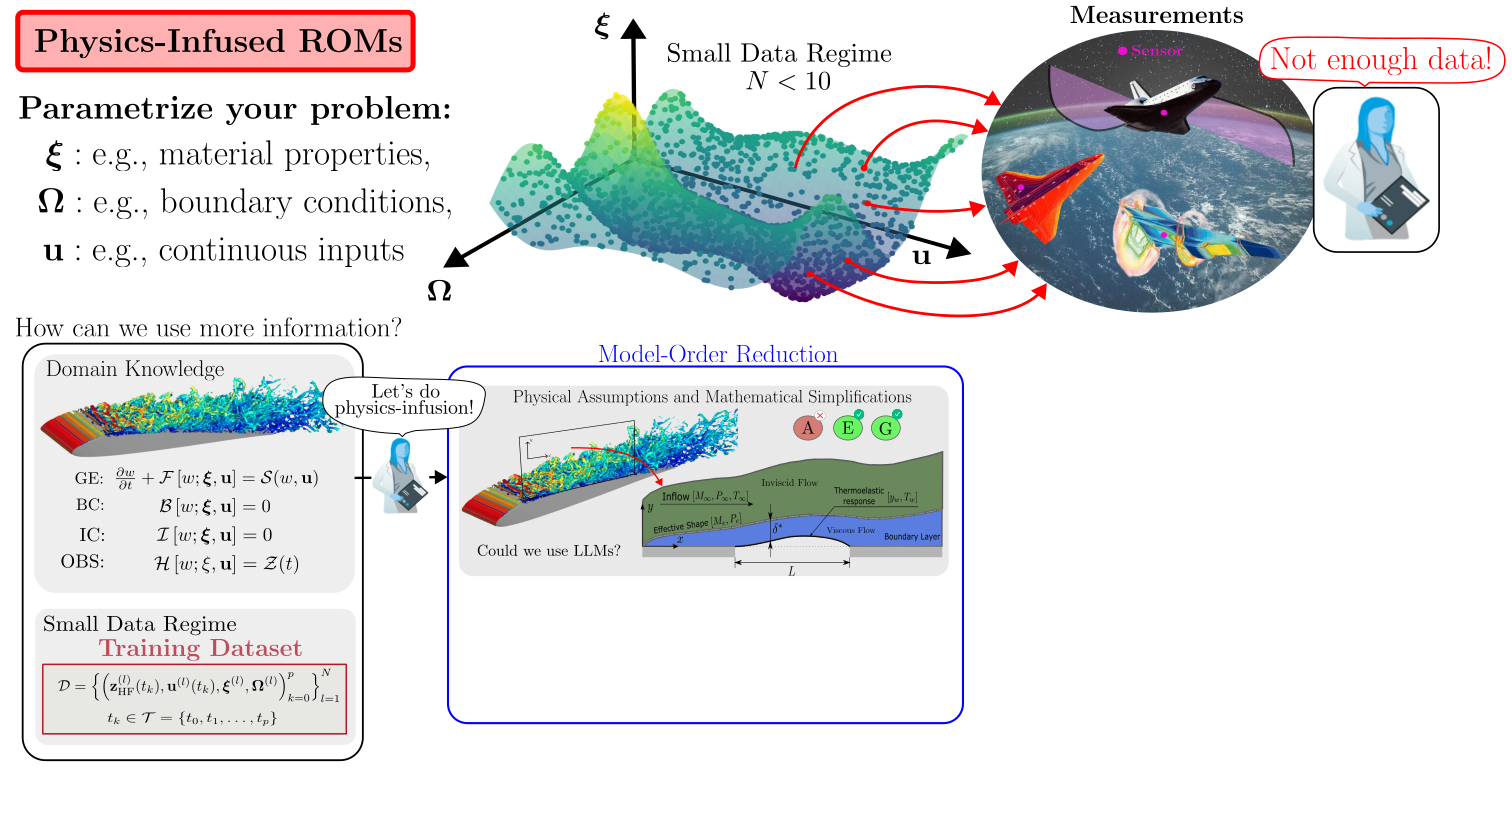
\includegraphics[width=0.9\textwidth]{../figs/sota/physics_infused_8.png}
    \end{figure}}
    \only<9>{
    \begin{figure}
        \centering
        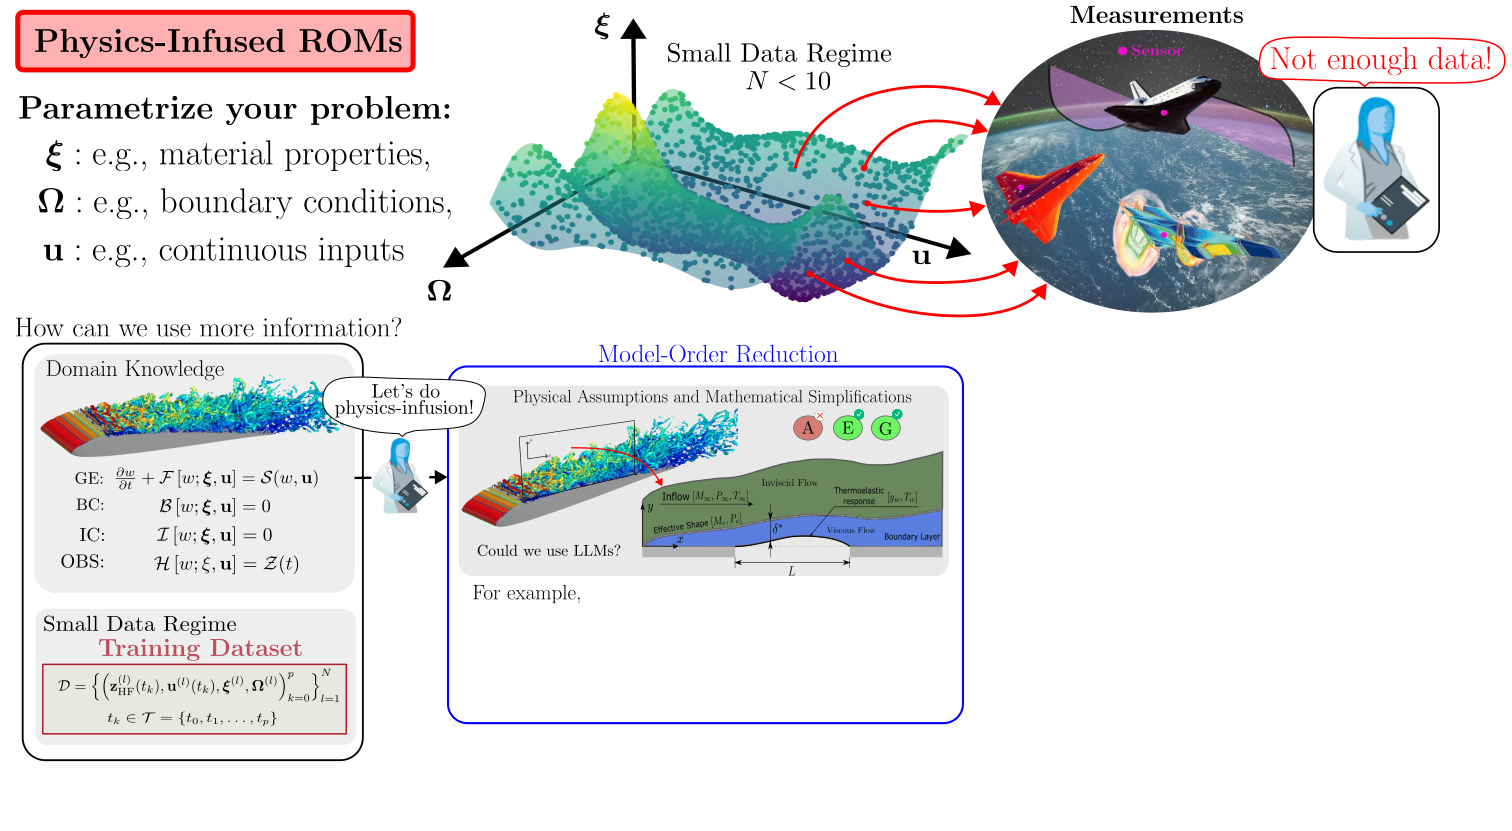
\includegraphics[width=0.9\textwidth]{../figs/sota/physics_infused_9.png}
    \end{figure}}
    \only<10>{
    \begin{figure}
        \centering
        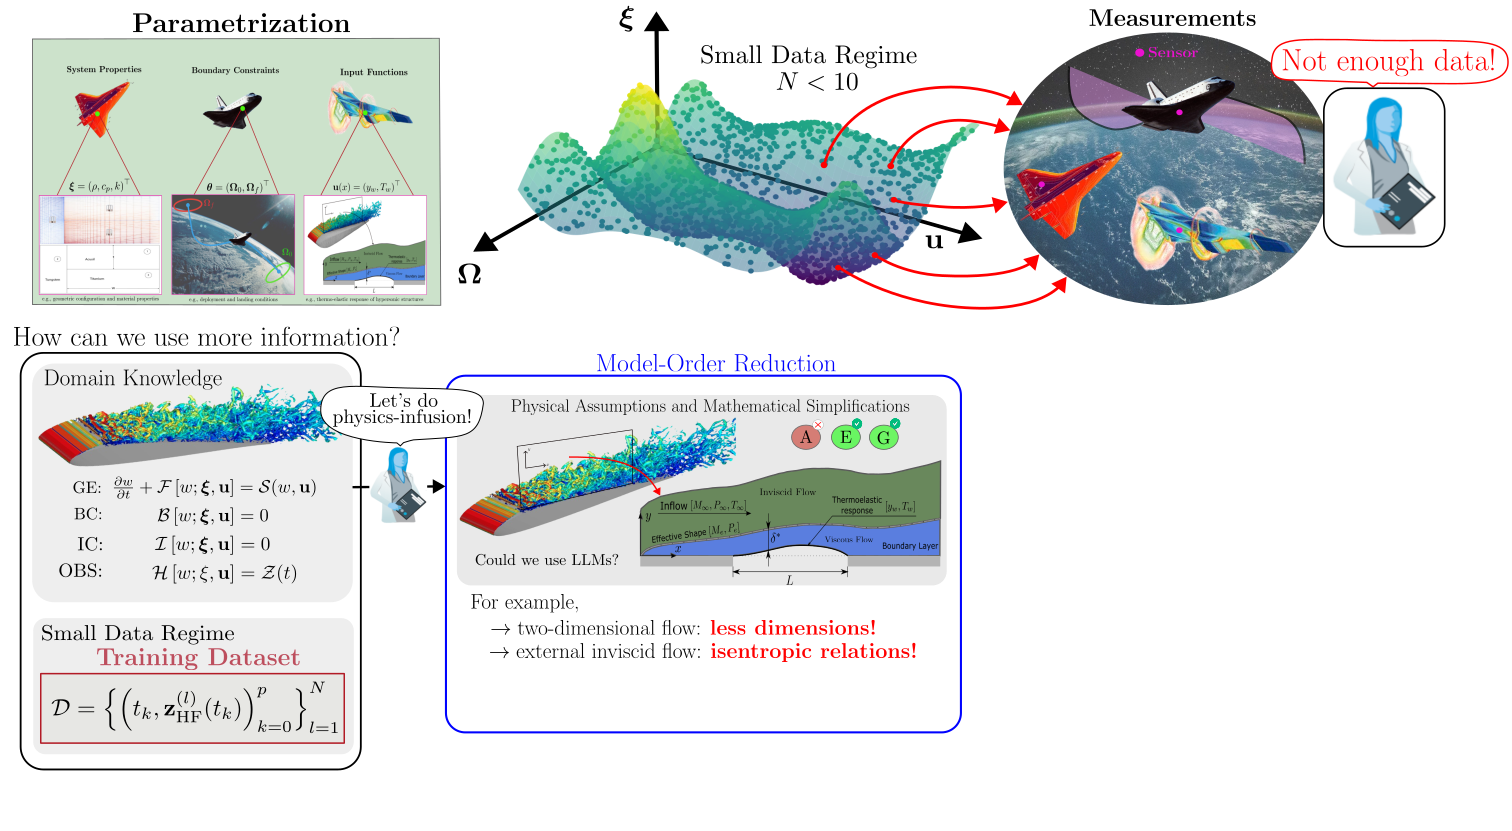
\includegraphics[width=0.9\textwidth]{../figs/sota/physics_infused_10.png}
    \end{figure}}
    \only<11>{
    \begin{figure}
        \centering
        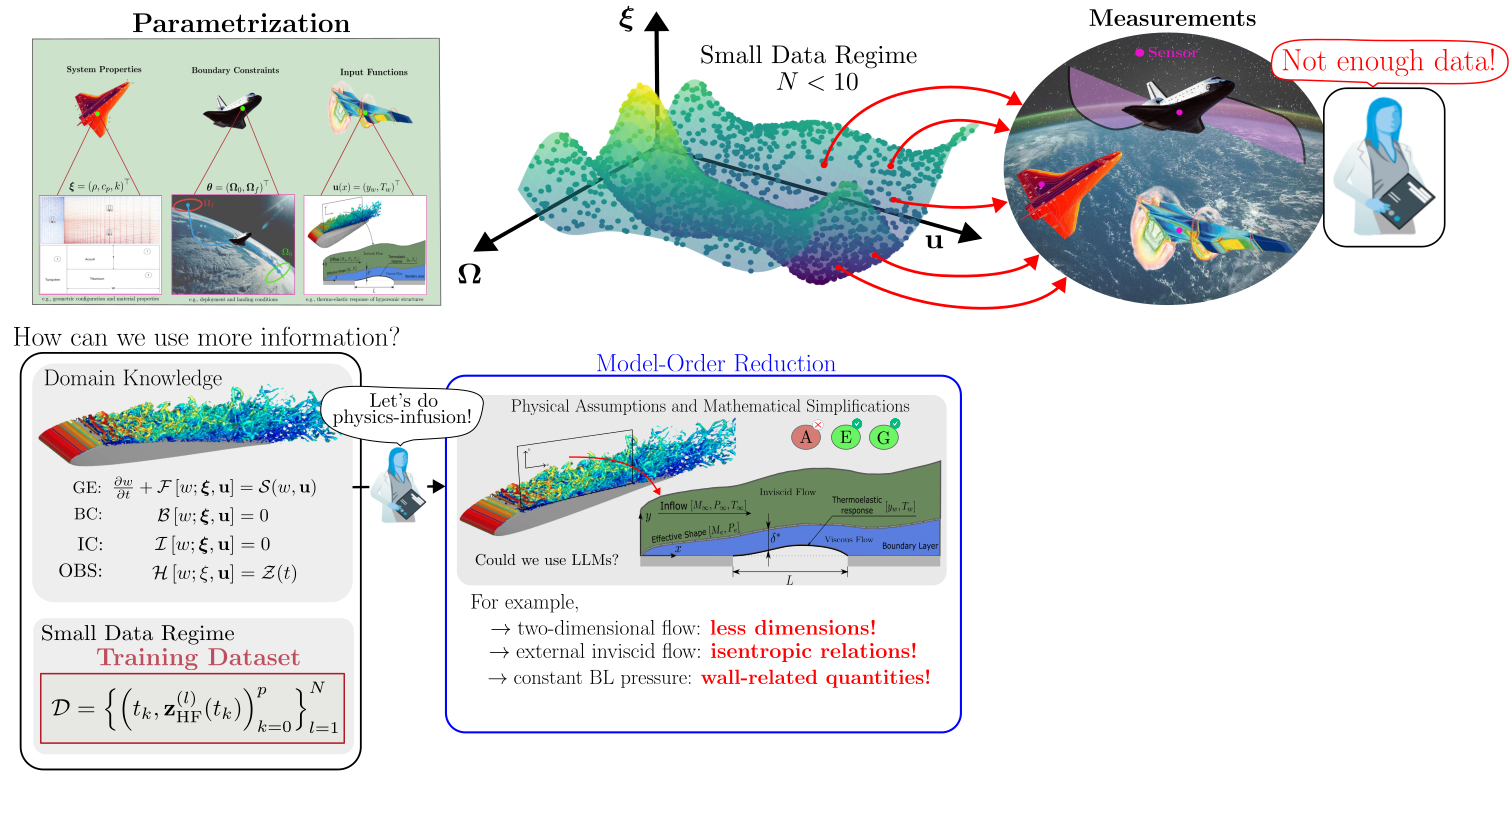
\includegraphics[width=0.9\textwidth]{../figs/sota/physics_infused_11.png}
    \end{figure}}
    \only<12>{
    \begin{figure}
        \centering
        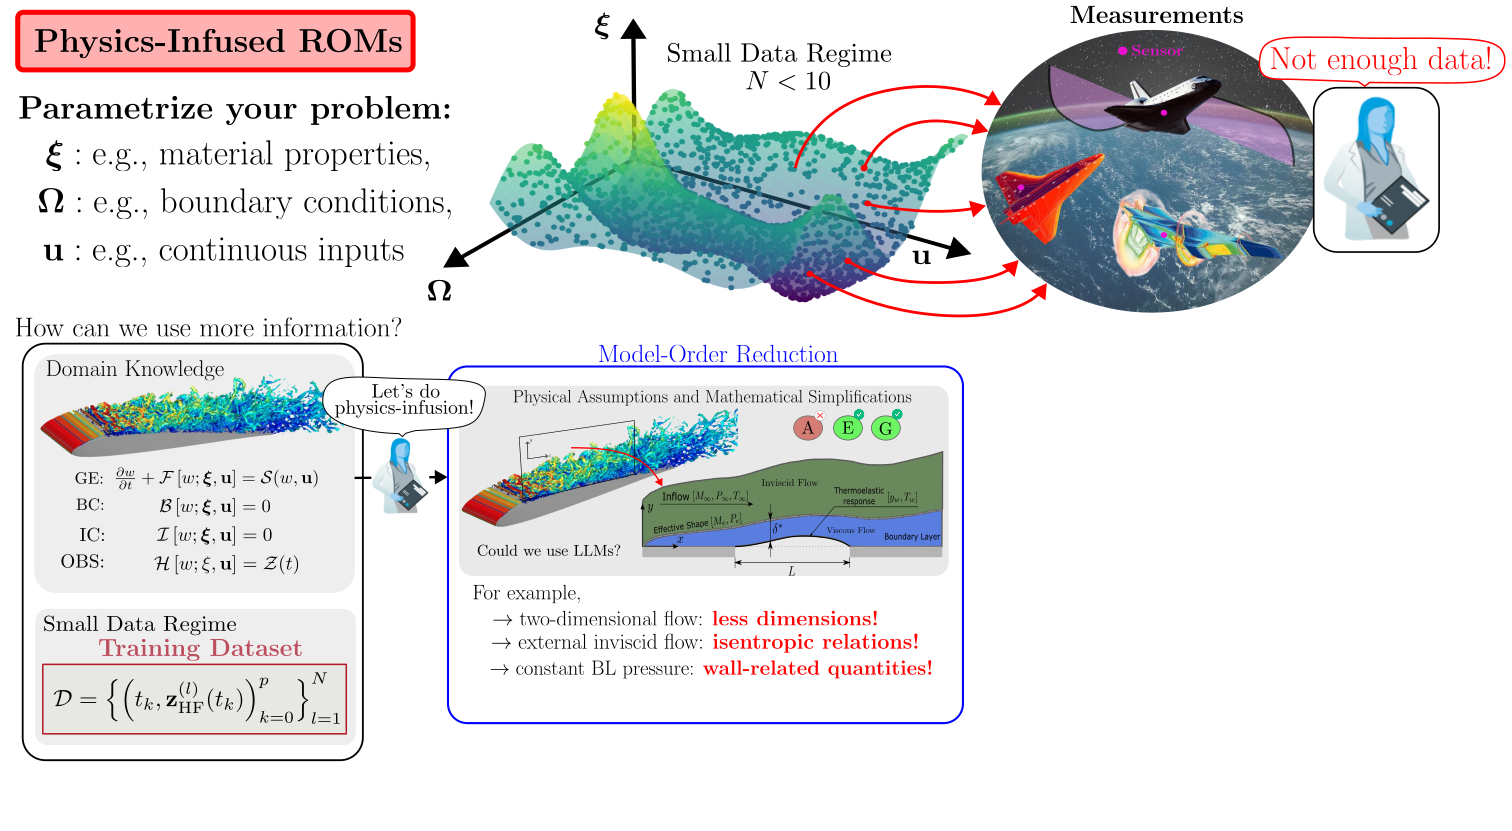
\includegraphics[width=0.9\textwidth]{../figs/sota/physics_infused_12.png}
    \end{figure}}
    \only<13>{
    \begin{figure}
        \centering
        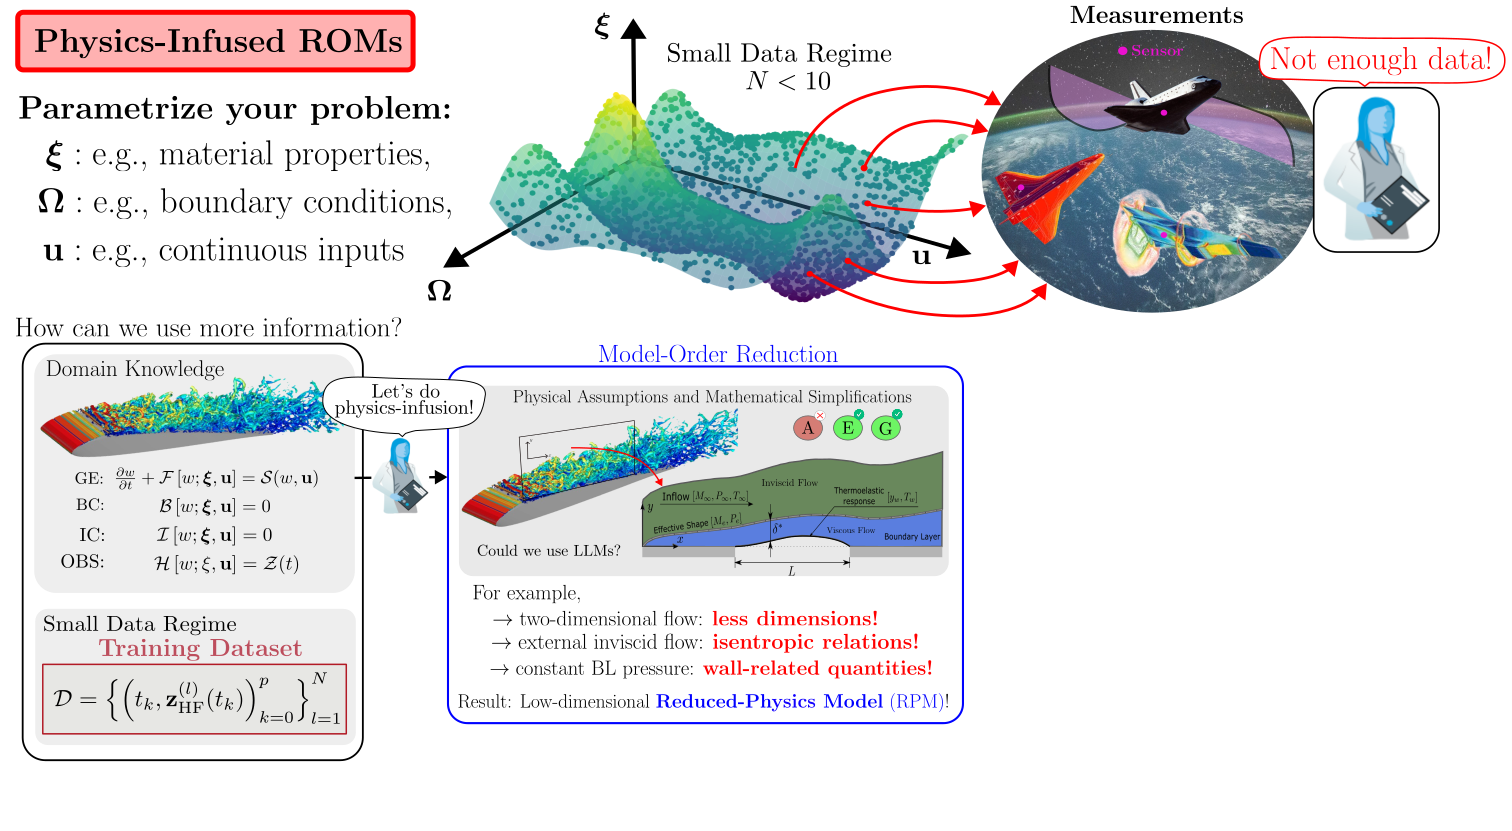
\includegraphics[width=0.9\textwidth]{../figs/sota/physics_infused_13.png}
    \end{figure}}
    \only<14>{
    \begin{figure}
        \centering
        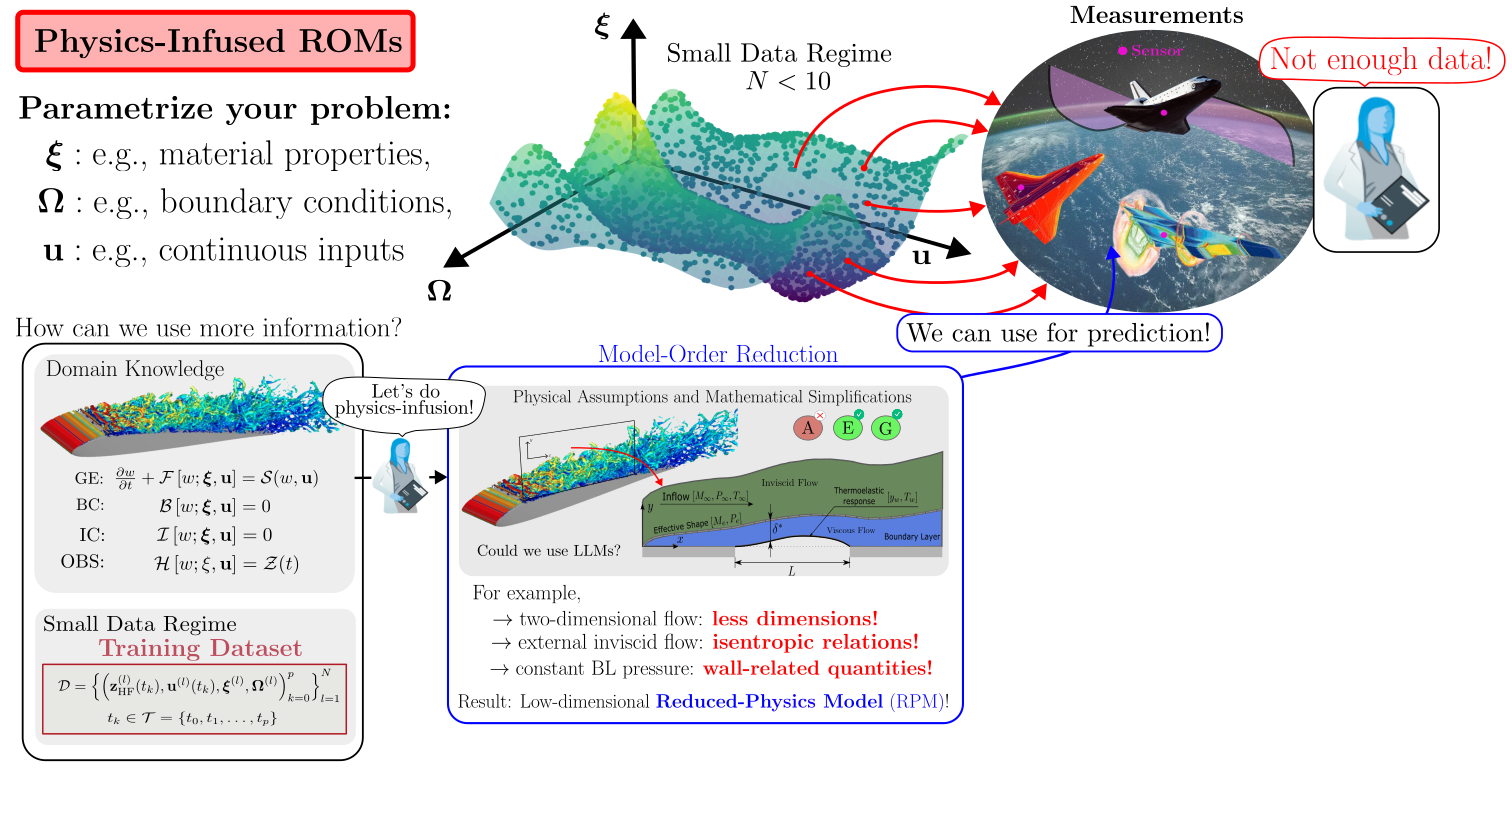
\includegraphics[width=0.9\textwidth]{../figs/sota/physics_infused_14.png}
    \end{figure}}
    \only<15>{
    \begin{figure}
        \centering
        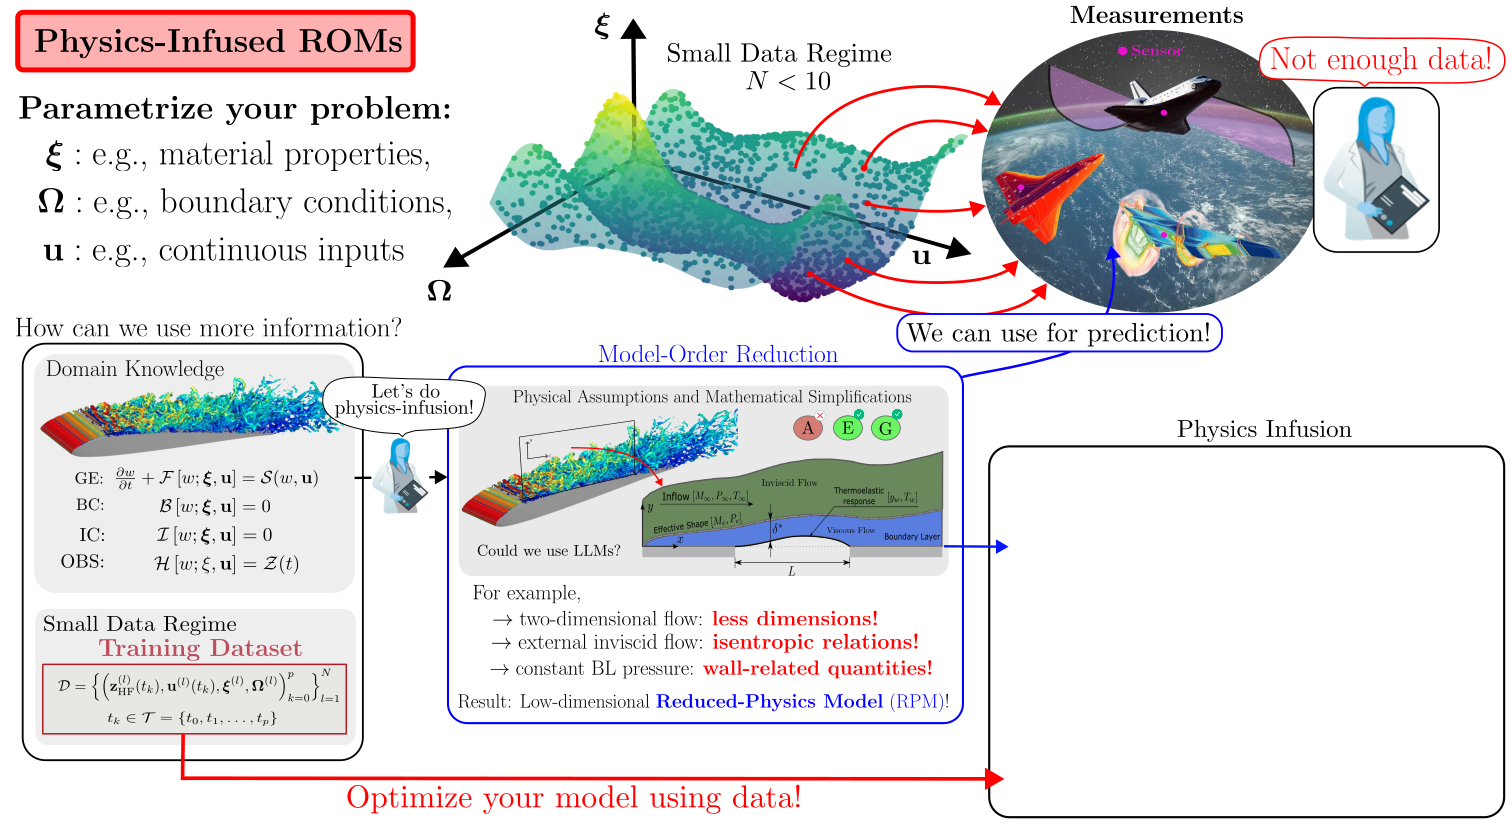
\includegraphics[width=0.9\textwidth]{../figs/sota/physics_infused_15.png}
    \end{figure}}
    \only<16>{
    \begin{figure}
        \centering
        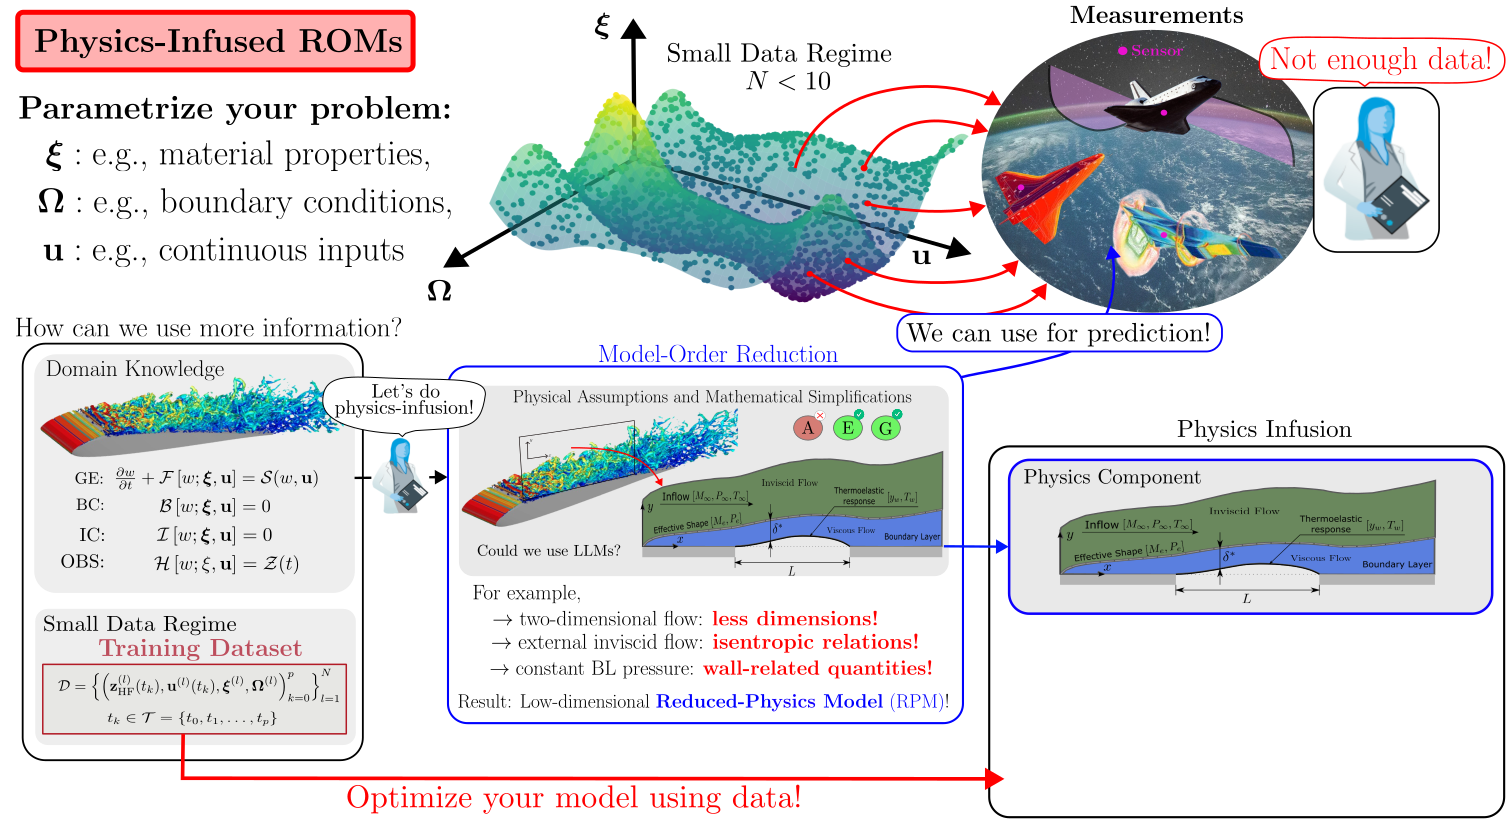
\includegraphics[width=0.9\textwidth]{../figs/sota/physics_infused_16.png}
    \end{figure}}
    \only<17>{
    \begin{figure}
        \centering
        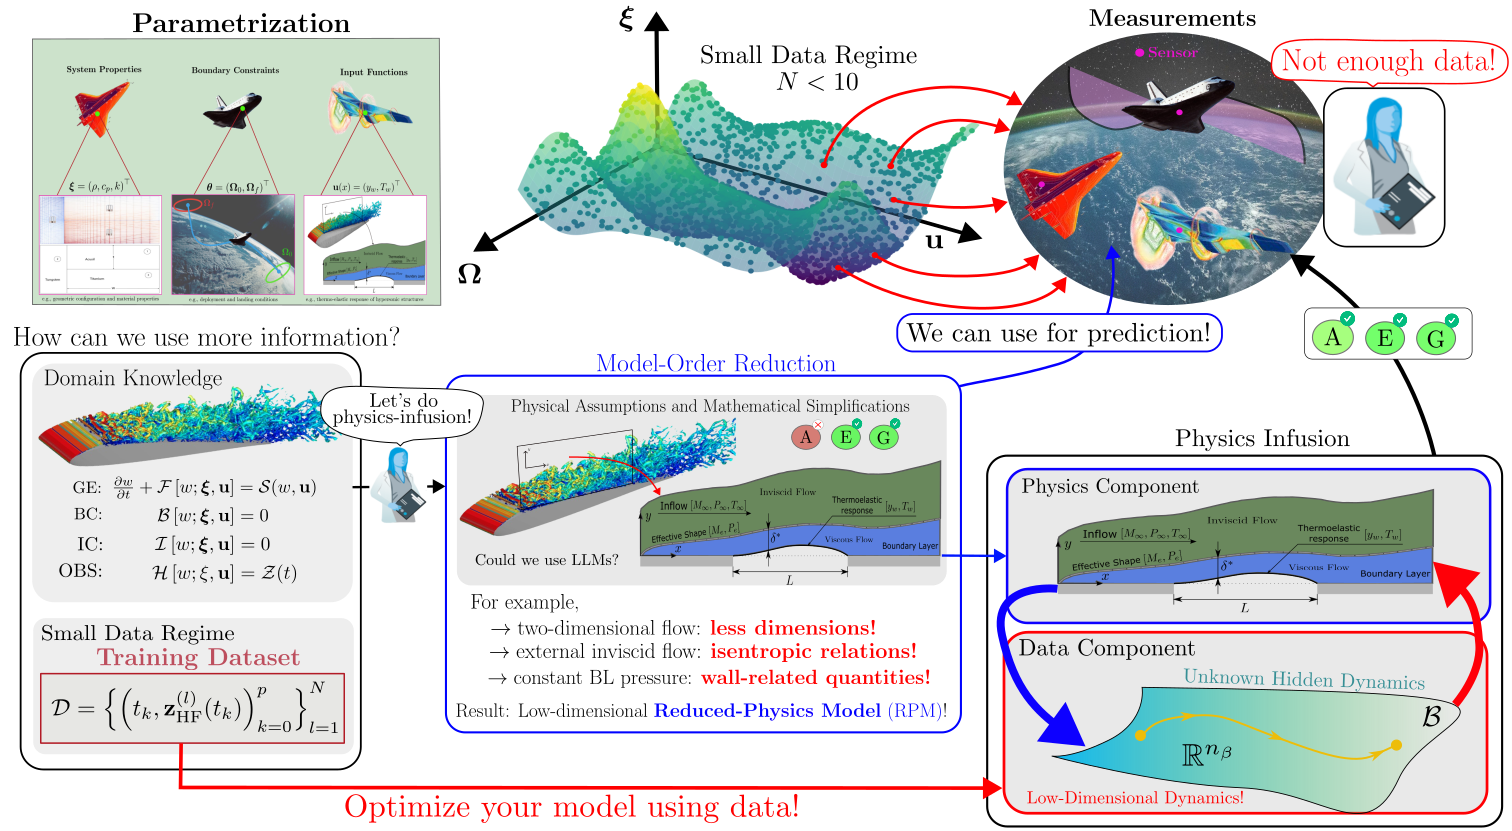
\includegraphics[width=0.9\textwidth]{../figs/sota/physics_infused_17.png}
    \end{figure}}
    \only<18>{
    \begin{figure}
        \centering
        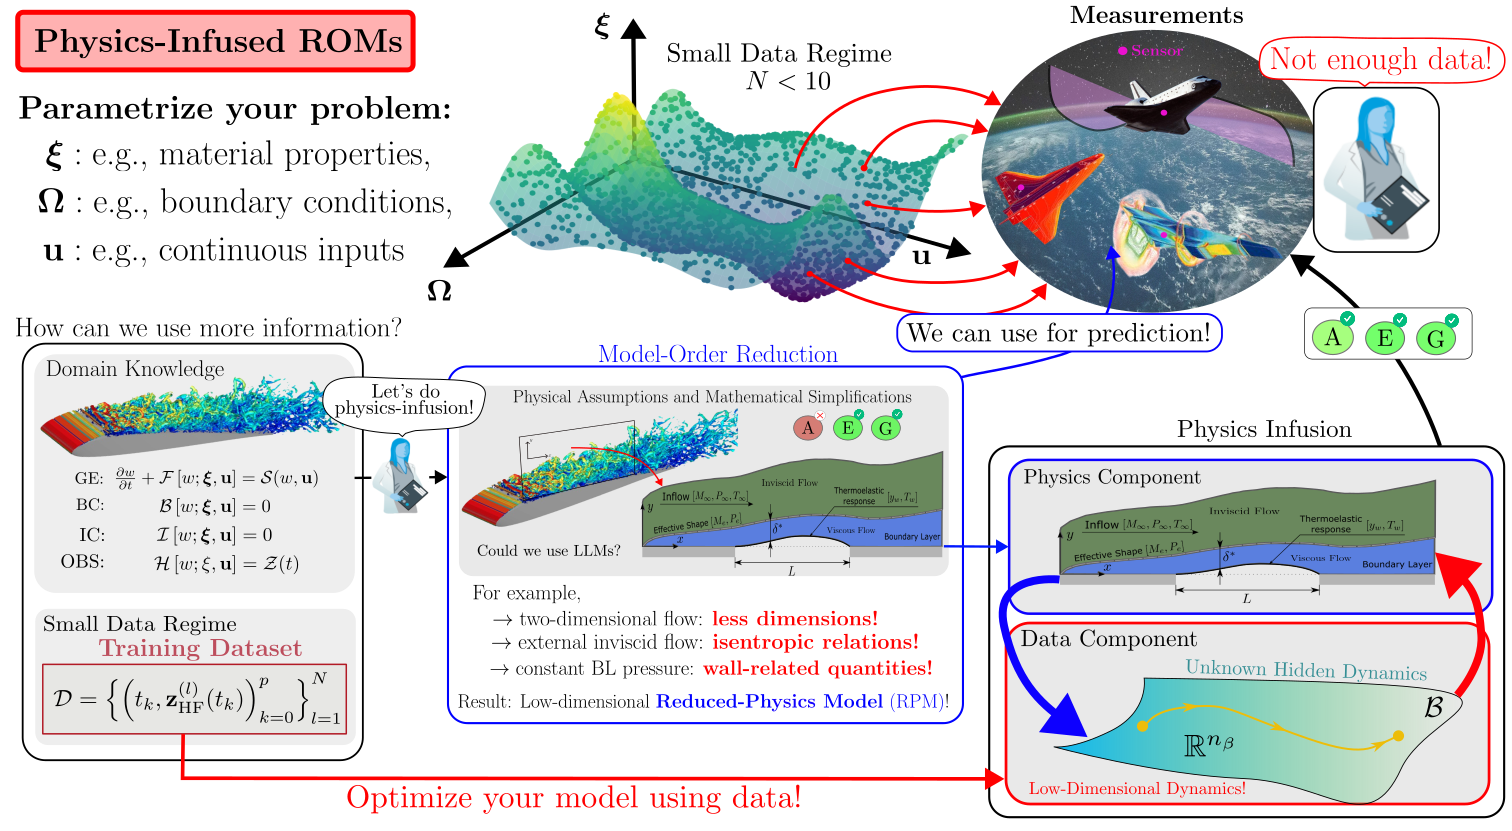
\includegraphics[width=0.9\textwidth]{../figs/sota/physics_infused_18.png}
    \end{figure}}
\end{frame}

\begin{frame}{\large Example: Hypersonic Thermal Protection Systems}
    \footnotesize
    \begin{columns}
        \visible<2->{
        \begin{column}{0.35\textwidth}
            \begin{graybox}{Semi-Discrete FOM}
                For example, FEM yields,
                \vspace*{-0.05in}
                \begin{align*}
                    \dot{\vu} &= \vF\left(\vu;\vp\right)\\
                    \vz_{\text{HF}} &= \vH\left(\vu;\vp\right)\\
                    \vu(t_0) &= \vu_0
                \end{align*}
                \vspace{-0.2in}
                \begin{enumerate}
                    \item<3-> $\vu\in\mathbb{R}^{n_u}$: states $(n_u\gg 1)$
                    \item<4-> $\vp\in\mathbb{R}^{n_p}$: parameters
                    \item<5-> $\vz_{\text{HF}}\in\mathbb{R}^{n_z}$: observable 
                \end{enumerate}
            \end{graybox}
        \end{column}}
        \hspace*{-0.2in}
        \visible<6->{
        \begin{column}{0.70\textwidth}
            \begin{graybox}{Coarse Graining (reduce FOM's complexity)}
                \hspace*{-0.08in}
                \begin{enumerate}
                    \item<7-> State decomposition $\vu = \left[\bvu,\delta\vu\right]^{\top}\in\mathbb{R}^{n_u}$ 
                    \begin{itemize}
                        \item<8-> Observables (e.g., averages) $\bvu\in\mathbb{R}^{n_{\bar{u}}}$
                        \item<9-> Un-observables (e.g., deviations) $\delta\vu\in\mathbb{R}^{n_{\delta u}}$ $\left(n_{\delta u}\gg n_{\bar{u}}\right)$
                    \end{itemize}
                    \item<10-> Projection operator $\cP:\cH_{n_u}\to\cH_{n_{\bar{u}}}\subset\cH_{n_u}$, e.g.,
                    \vspace*{-0.1in}
                    \begin{equation*}
                        \cP: \cG\left(\vu\right)\rightarrow \bar{\cG}\left(\bvu\right)\rightarrow\text{cheaper to evaluate!}
                        \vspace*{-0.1in}
                    \end{equation*}
                    \item<11-> Complement operator $\cQ = \cI - \cP$
                \end{enumerate}
                \vspace{-0.1in}
                \visible<12->{
                \begin{figure}
                    \centering
                    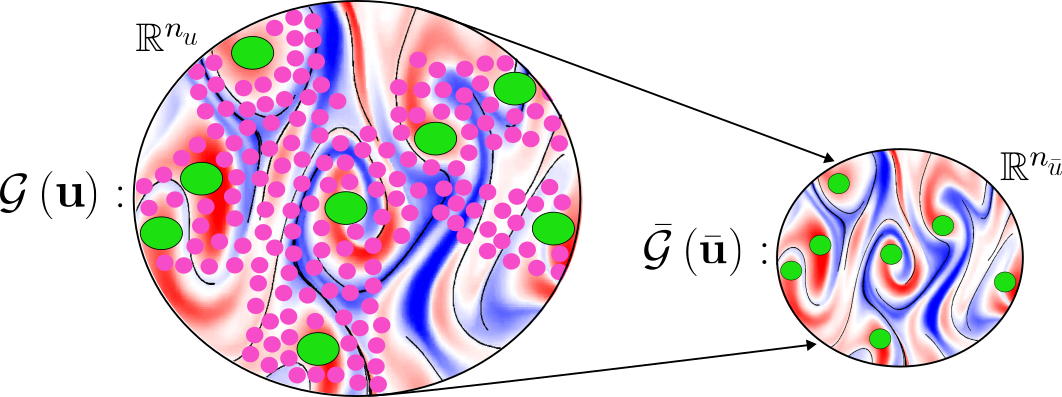
\includegraphics[width=0.65\textwidth]{../figs/pirom/coarse_graining.png}
                \end{figure}}
                \vspace*{-0.1in}
            \end{graybox}
        \end{column}}
    \end{columns}
\end{frame}

\begin{frame}{Addressing the ITM: Coarse Graining}
    \footnotesize
    \visible<1->{
        \textbf{For example}, we can apply \textbf{coarse-graining} principles to \textbf{hypersonic TPS} models {\tiny [2,3]},}
    \vspace*{-0.1in}
    \begin{columns}
        \visible<1->{
        \begin{column}{0.55\textwidth}
            \only<1>{
                \begin{figure}
                    \centering
                    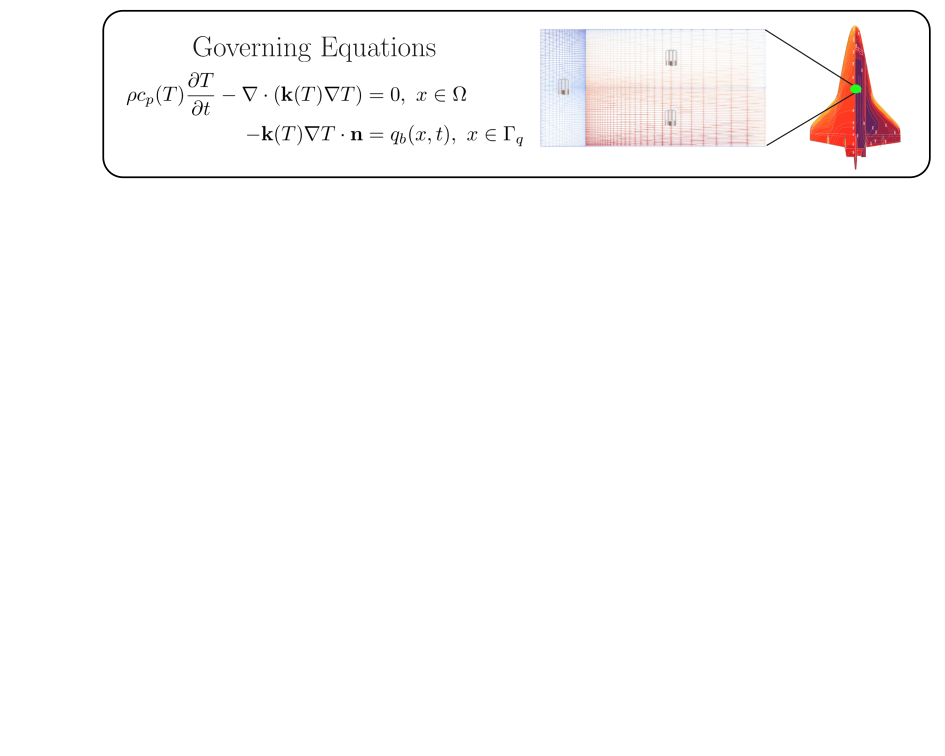
\includegraphics[width=0.85\textwidth]{../figs/pirom/coarse_graining_tps_left_1.png}
                \end{figure}}
            \only<2>{
                \begin{figure}
                    \centering
                    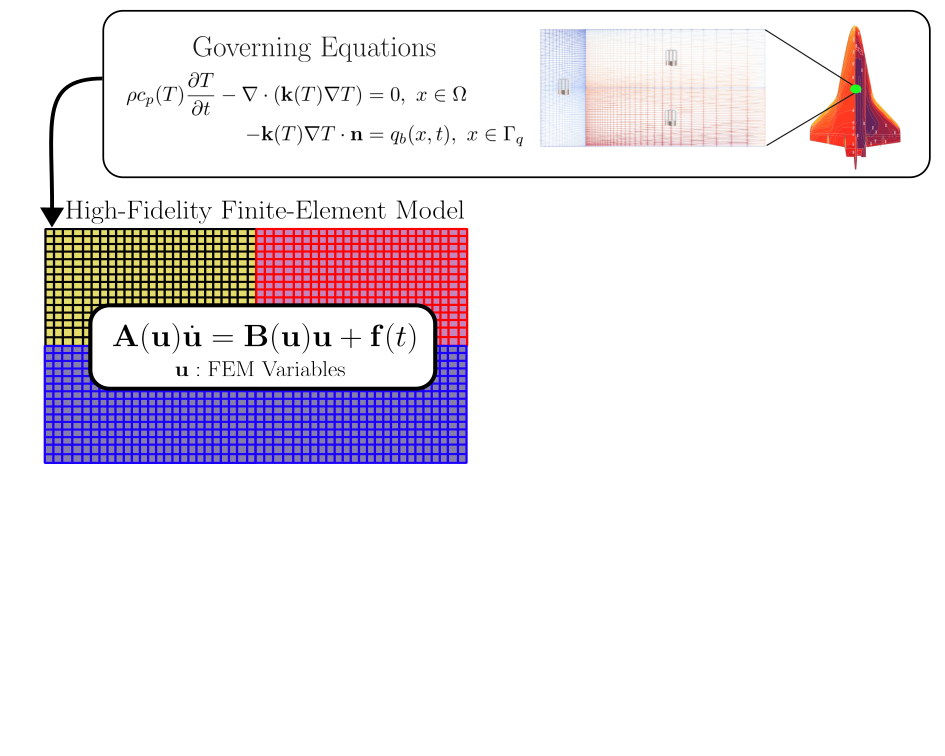
\includegraphics[width=0.85\textwidth]{../figs/pirom/coarse_graining_tps_left_2.png}
                \end{figure}}
            \only<3>{
                \begin{figure}
                    \centering
                    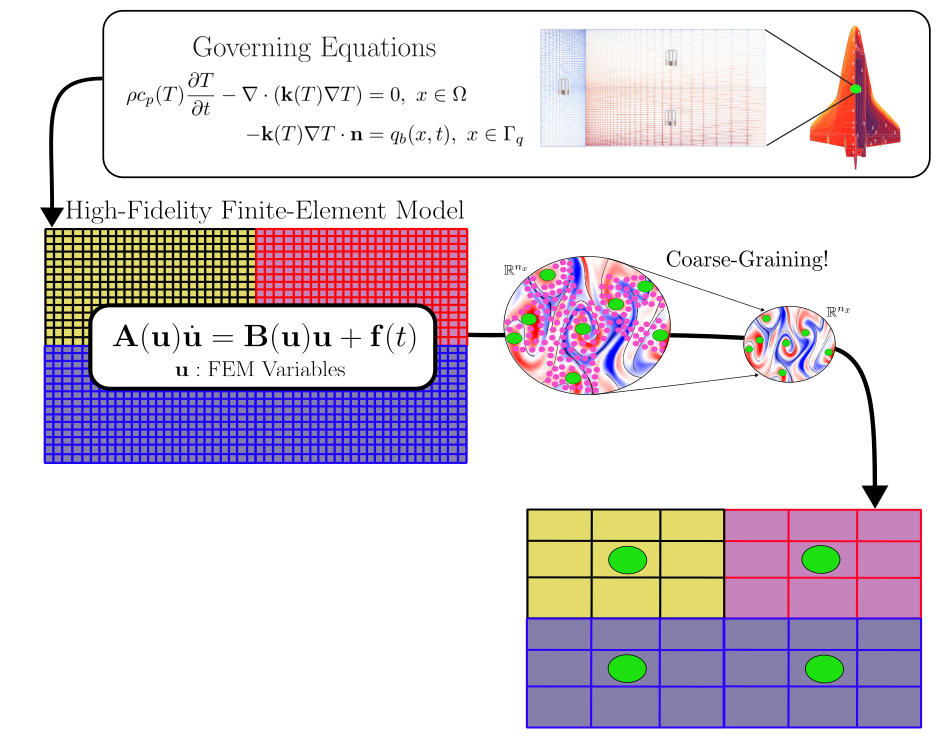
\includegraphics[width=0.85\textwidth]{../figs/pirom/coarse_graining_tps_left_3.png}
                \end{figure}}
            \only<4->{
                \begin{figure}
                    \centering
                    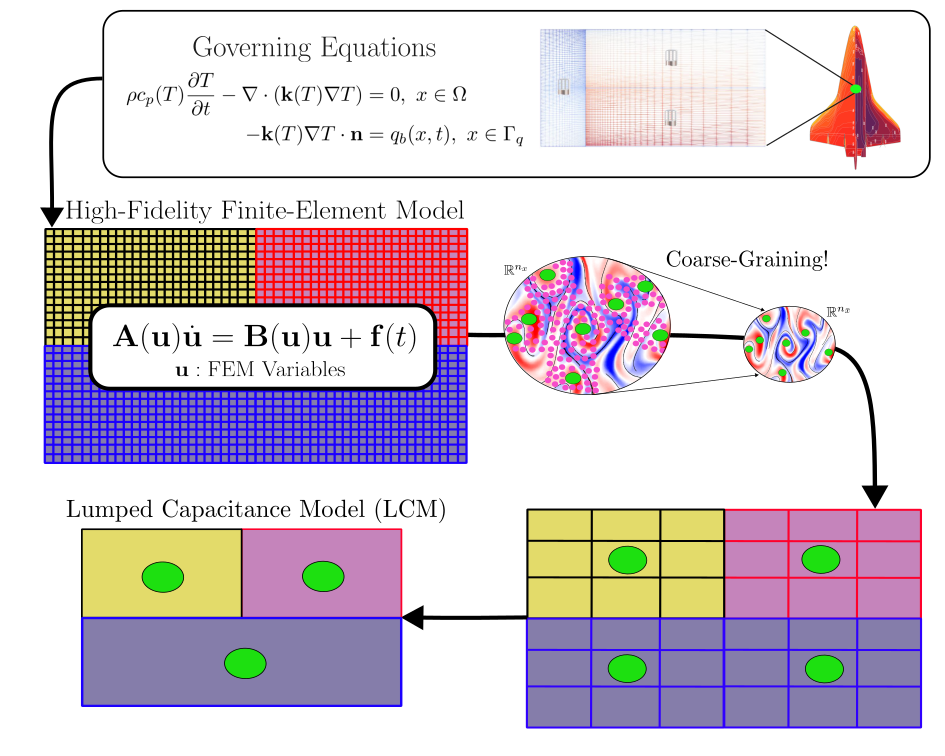
\includegraphics[width=0.85\textwidth]{../figs/pirom/coarse_graining_tps_left_4.png}
                \end{figure}}
        \end{column}}
        \hspace*{-0.25in}
        \visible<1->{
        \begin{column}{0.55\textwidth}
            \vspace*{-0.05in}
            \only<5>{
                \begin{figure}
                    \centering
                    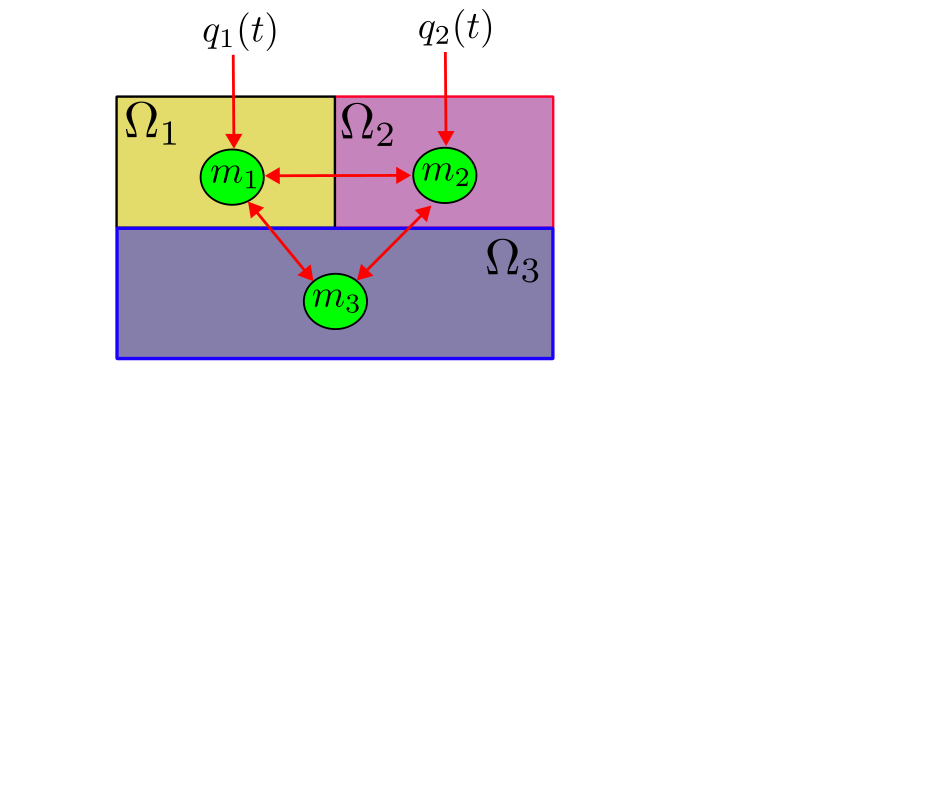
\includegraphics[width=0.95\textwidth]{../figs/pirom/coarse_grained_variables_tps_1.png}
                \end{figure}}
            \only<6>{
                \begin{figure}
                    \centering
                    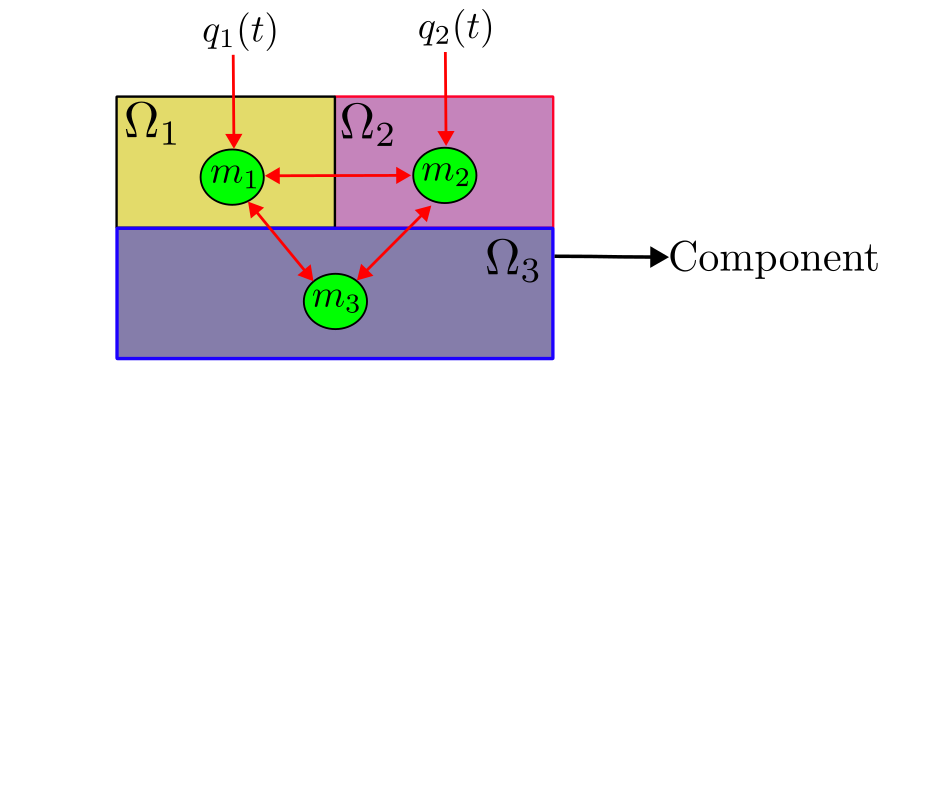
\includegraphics[width=0.95\textwidth]{../figs/pirom/coarse_grained_variables_tps_2.png}
                \end{figure}}
            \only<7>{
                \begin{figure}
                    \centering
                    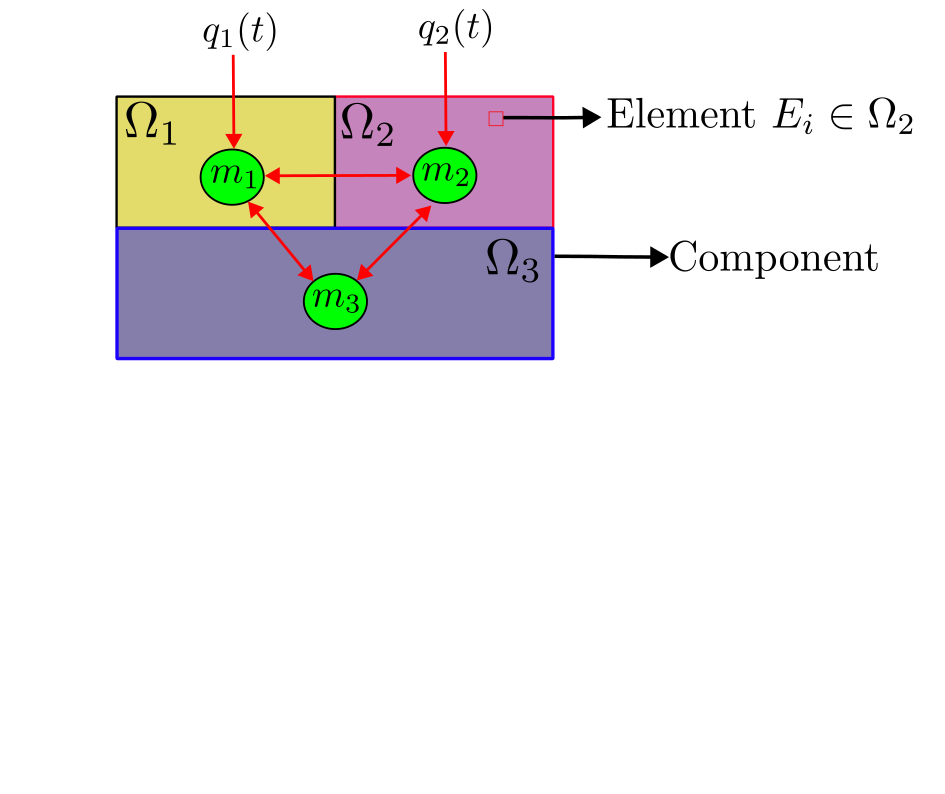
\includegraphics[width=0.95\textwidth]{../figs/pirom/coarse_grained_variables_tps_3.png}
                \end{figure}}
            \only<8>{
                \begin{figure}
                    \centering
                    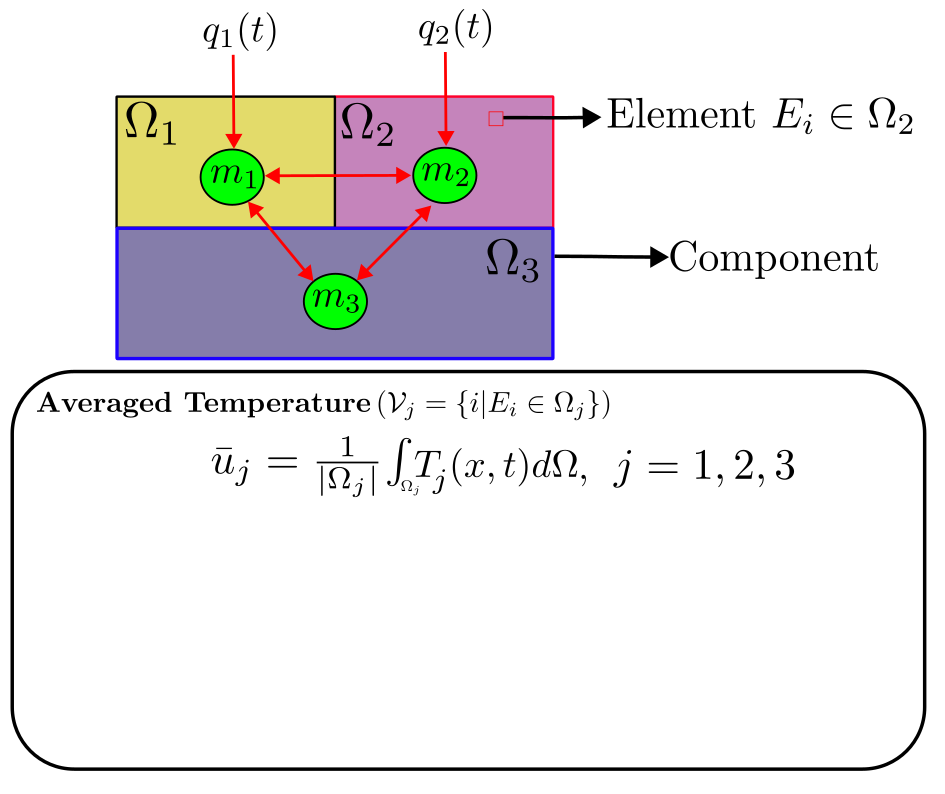
\includegraphics[width=0.95\textwidth]{../figs/pirom/coarse_grained_variables_tps_4.png}
                \end{figure}}
            \only<9>{
                \begin{figure}
                    \centering
                    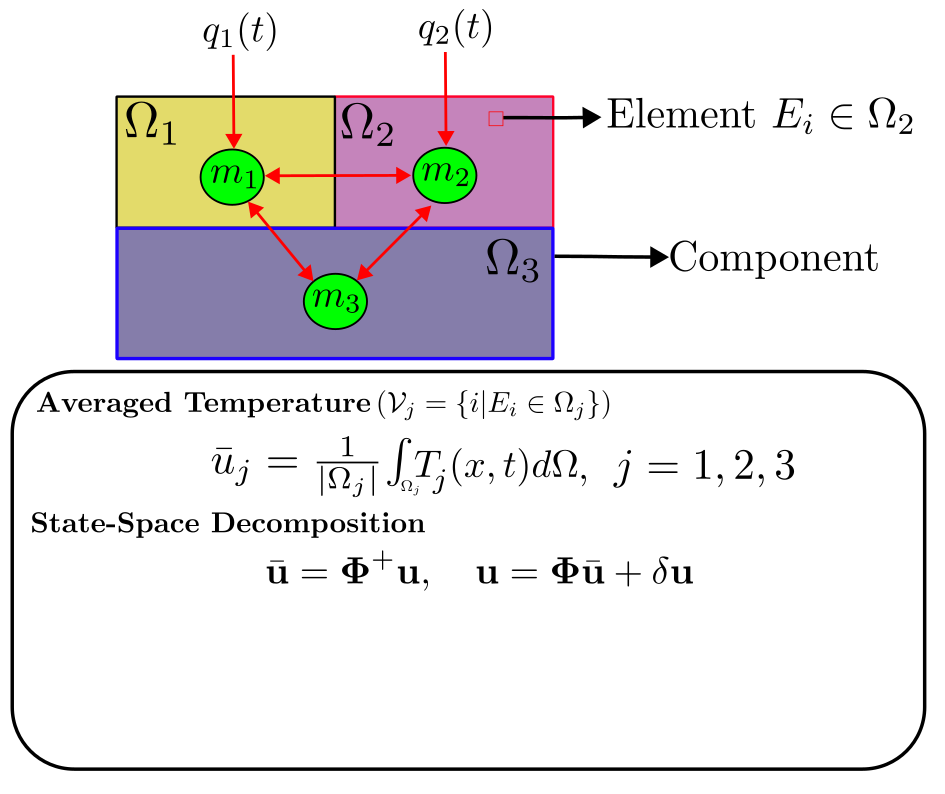
\includegraphics[width=0.95\textwidth]{../figs/pirom/coarse_grained_variables_tps_5.png}
                \end{figure}}
            \only<10>{
                \begin{figure}
                    \centering
                    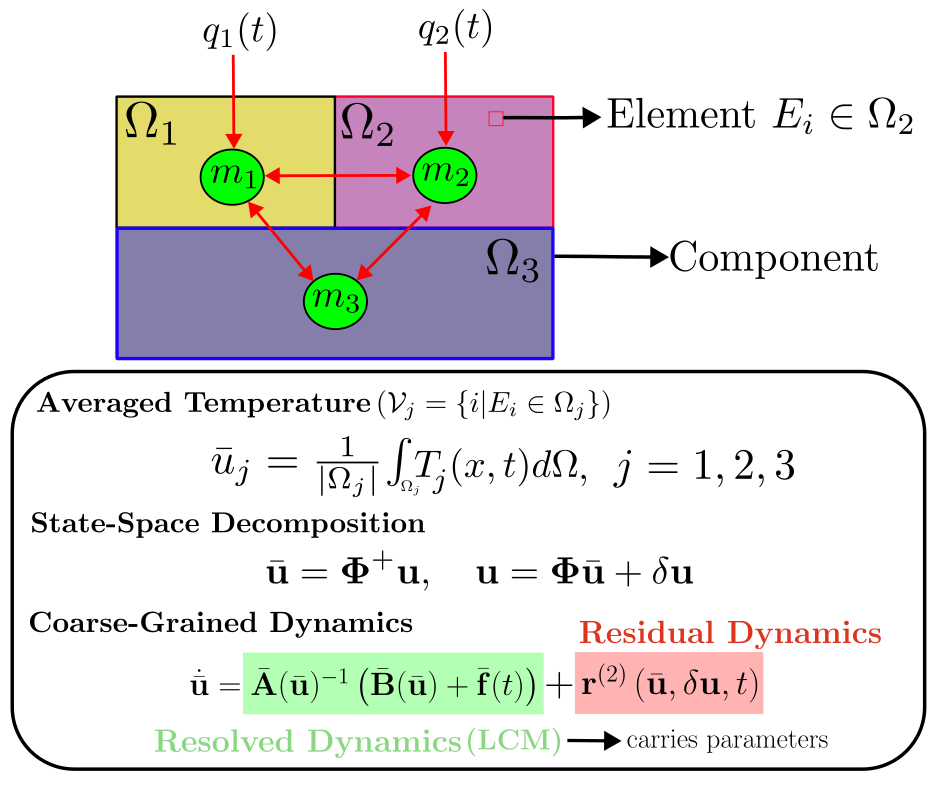
\includegraphics[width=0.95\textwidth]{../figs/pirom/coarse_grained_variables_tps_6.png}
                \end{figure}}
        \end{column}}
    \end{columns}
\end{frame}

\begin{frame}{Addressing the ITM: Physics Infusion}
    \footnotesize
    \visible<1->{
        Mori-Zwanzig (MZ) connects the \textbf{averaged} and \textbf{residual} dynamics for \textbf{physics-infusion} {\tiny [2]},}
    \visible<2->{
    \begin{equation*}
        \text{Projected GLE}:\quad \underbrace{\frac{\partial}{\partial t} \cP e^{t\cL}\bvu}_{\text{Observable Dynamics}} \visible<3->{= \underbrace{\cP e^{t\cL}\cP\cL\bvu}_{\text{Markovian}}} \visible<4->{+ \cP\underbrace{\int_0^t e^{(t-s)\cL}\cP\cL e^{s\cQ\cL}\cQ\cL\bvu ds}_{\text{Non-Markovian}}} \visible<5->{+ \cP\underbrace{e^{t\cQ\cL}\cQ\cL\bvu}_{\text{Noise}}}
    \end{equation*}}
    \begin{columns}
        \visible<3->{
        \begin{column}{0.3\textwidth}
            \centering
            \textbf{Markovian}
            \begin{figure}
                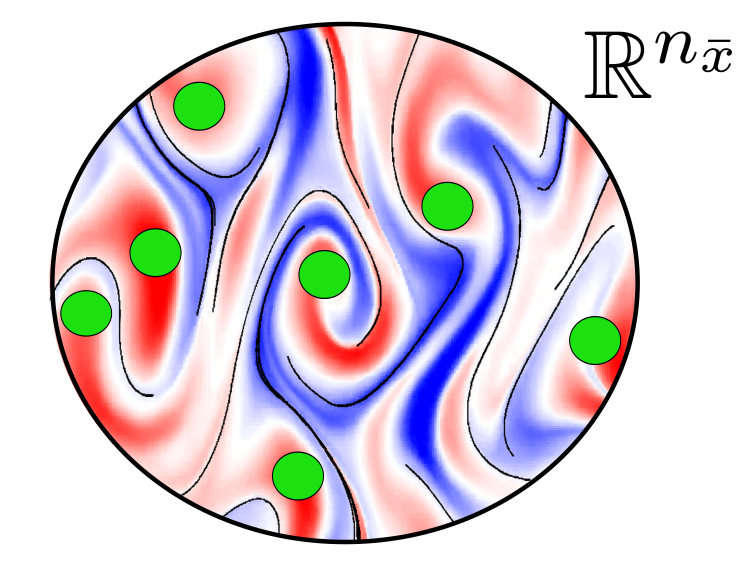
\includegraphics[width=0.9\textwidth]{../figs/pirom/coarse_variables.png}
            \end{figure}
            {\small (known dynamics)}
        \end{column}}
        \visible<4->{
        \begin{column}{0.3\textwidth}
            \centering
            \textbf{Non-Markovian}
            \begin{figure}
                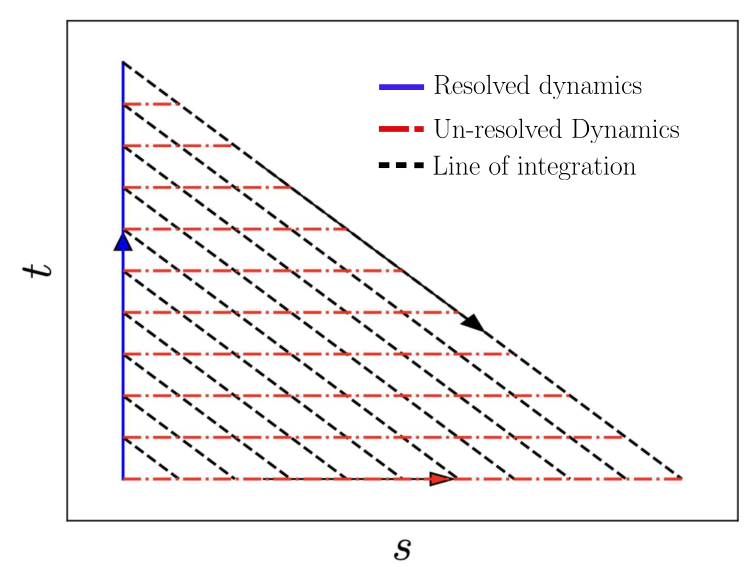
\includegraphics[width=0.9\textwidth]{../figs/pirom/memory.png}{\tiny [1]}
            \end{figure}
            {\small\textcolor{red}{(unknown dynamics)}}
        \end{column}}
        \visible<5->{
        \begin{column}{0.3\textwidth}
            \centering
            \textbf{Noise}
            \begin{figure}
                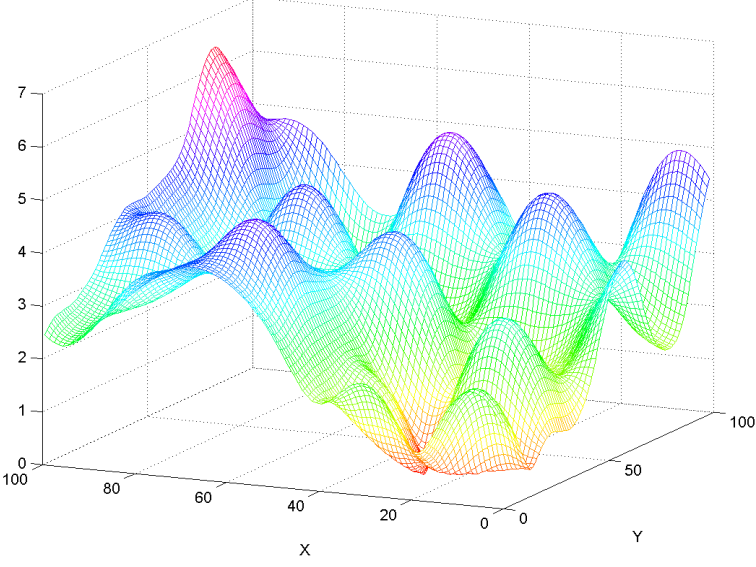
\includegraphics[width=0.9\textwidth]{../figs/pirom/noise.png}
            \end{figure}
            {\small\textcolor{black}{(orthogonal to $\cP$)}}
        \end{column}}
    \end{columns}
    \begin{center}
        {\tiny GLE: Generalized Langevin Equation, $\cL$: Liouville operator, PGLE: Projected GLE}
    \end{center}
\end{frame}

\begin{frame}{\large Approximate the Memory Kernel for Physics Infusion}
    \footnotesize
    \begin{columns}
        \begin{column}{0.5\textwidth}
            \visible<2->{
            \begin{graybox}{Memory Kernel Parametrization}
                \visible<3->{
                Define the memory kernel,
                \begin{equation*}
                    \vkappa(\bvu,t,s) = \cP e^{(t-s)\cL}\cP\cL e^{s\cQ\cL}\cQ\cL\bvu
                \end{equation*}}
                \visible<4->{
                Parametrize the \textbf{memory kernel},
                \vspace*{-0.05in}
                \begin{equation*}
                    \vkappa(\bvu,t,s;\redvTheta) \approx \sum_{j=1}^{m} \cK_j(t,s,\bvu;\redvTheta)\phi_j(s,\bvu;\redvTheta)
                \end{equation*}}
                \vspace*{-0.05in}
                \visible<5->{
                For \textbf{TPS problem}, design $\cK_j$ and $\phi_j$ as,
                \vspace*{-0.05in}
                \begin{align*}
                    \cK_j(t,s,\bvu;\redvTheta) &= e^{-\textcolor{red}{\lambda_j}(t-s)}\Rightarrow\text{{\tiny \textbf{exponential decay!}}}\\
                    \phi_j(s,\bvu;\redvTheta) &= \textcolor{red}{\vp_j}\left(\textcolor{red}{\vq_j}^\top\bar{\vu}(s) + \textcolor{red}{\vr_j}^\top\underbrace{\bar{\vf}(s)}_{\text{external forcing}} \right)
                \end{align*}}
            \end{graybox}}
        \end{column}
        \hspace*{-0.1in}
        \begin{column}{0.55\textwidth}
            \visible<6->{
            \begin{graybox}{Markovian Reformulation}
                \visible<7->{
                Define the \textbf{memory variables} as,
                \vspace*{-0.05in}
                \begin{equation*}
                    \beta_j(t) = \int_0^t e^{-\textcolor{red}{\lambda_j}(t-s)} \left(\textcolor{red}{\vq_j}^\top\bar{\vu}(s) + \textcolor{red}{\vr_j}^\top\bar{\vf}(s)\right) ds
                \end{equation*}}
                \visible<8->{
                so that the \textbf{hidden dynamics} are,
                \vspace*{-0.05in}
                \begin{equation*}
                    \dot{\beta}_j = \textcolor{red}{\lambda_j}\beta_j + \textcolor{red}{\vq_j}^\top\bar{\vu} + \textcolor{red}{\vr_j}^\top\bar{\vf},\:\: j=1,\dots,m
                \end{equation*}}
                \visible<9->{
                Thus, \textbf{the PIROM may be written as},
                \vspace*{-0.05in}
                \begin{align*}
                    \dot{\bvu} &= \underbrace{\cP e^{t\cL}\cP\cL\bvu}_{\text{\textbf{LCM dynamics!}}} + \sum_{j=1}^{m}\textcolor{red}{\vp_j}\beta_j\\
                    \vspace*{-0.01in}
                    \dot{\beta}_j &= \textcolor{red}{\lambda_j}\beta_j + \textcolor{red}{\vq_j}^\top\bar{\vu} + \textcolor{red}{\vr_j}^\top\bar{\vf}\\
                    \vspace*{-0.01in}
                    \vz &= \textcolor{red}{\vD_{\bar{u}}}\bvu + \textcolor{red}{\vD_{\beta}}\boldsymbol{\beta}
                    \vspace*{-0.05in}
                \end{align*}}
                \visible<10->{
                \vspace*{-0.05in}
                $\redvTheta = \left\{\textcolor{red}{\vP,\vQ,\vLambda,\vR,\vD_{\bar{u}},\vD_{\beta}}\right\}$ learnable parameters}
                \vspace*{0.05in}
            \end{graybox}}
        \end{column}
    \end{columns}
\end{frame}

\begin{frame}{\large Learning the Hidden Dynamics}
    \footnotesize
    \begin{columns}
        \begin{column}{0.6\textwidth}
            \centering
            \vspace*{-0.2in}
            \only<9>{
            \begin{figure}
                \centering
                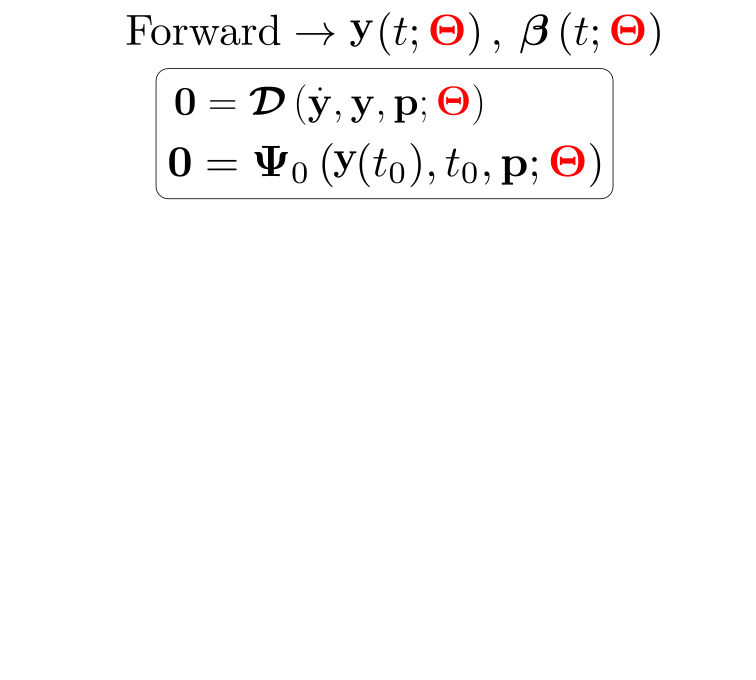
\includegraphics[width=0.7\textwidth]{../figs/pirom/adjoint_gradient_1.png}
            \end{figure}}
            \only<10>{
            \begin{figure}
                \centering
                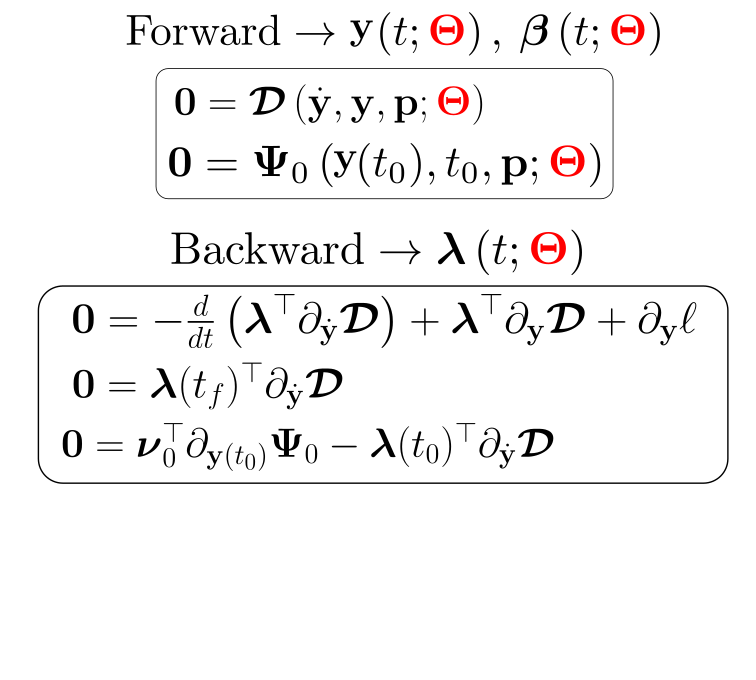
\includegraphics[width=0.7\textwidth]{../figs/pirom/adjoint_gradient_2.png}
            \end{figure}}
            \only<11>{
            \begin{figure}
                \centering
                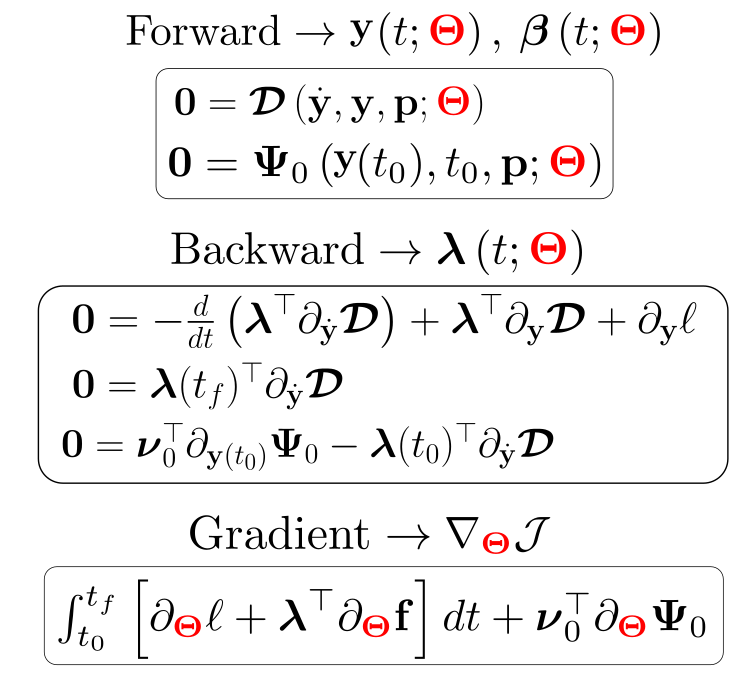
\includegraphics[width=0.7\textwidth]{../figs/pirom/adjoint_gradient_3.png}
            \end{figure}}
        \end{column}
        \hspace*{-0.5in}
        \begin{column}{0.45\textwidth}
            \visible<2->{
            \begin{graybox}{Constrained Parameter Opt.}
                \vspace*{-0.1in}
                \begin{align*}
                    \vspace*{0.05in}
                    \visible<3->{
                    \min_{\redvTheta} &\quad \cJ\left(\redvTheta\right) = \frac{1}{N} \sum_{l=1}^{N}\int_{t_0}^{t_f}\ell^{(l)}dt}\\
                    \visible<7->{
                    \text{s.t.} &\quad \vzero = \boldsymbol{\mathcal{D}}\left(\vy^{(l)},\dot{\vy}^{(l)},\vp^{(l)};\redvTheta\right)}\\
                    \visible<8->{
                    &\quad \boldsymbol{0} = \vPsi_0\left(\vy^{(l)}(t_0),t_0;\redvTheta\right)}
                \end{align*}
                \vspace*{-0.2in}
                \begin{itemize}
                    \item<4-> $\ell^{(l)} = \left\|\vz^{(l)} - \vz_{\text{HF}}^{(l)}\right\|_2^2$
                    \vspace*{-0.02in}
                    \item<5-> $\vz_{\text{HF}},\vz$ HF and PIROM observables,
                    \vspace*{-0.02in}
                    \item<6-> $\vy = \left[\bar{\vu},\vbeta\right]^\top$ PIROM state, 
                    \vspace*{-0.02in}
                    \item<7-> $\vcD$: PIROM compact dynamics,
                    \vspace*{-0.02in}
                    \item<8-> $\vPsi_0$: initial condition.
                    \vspace*{-0.1in}
                \end{itemize}
                \hspace*{-0.1in}
            \end{graybox}}
        \end{column}
    \end{columns}
\end{frame}

% % part 3: resolving the impossible trinity of optimal control (ITOC)
% \begin{frame}{Content Overview}
%     \footnotesize
%     \begin{enumerate}
%         \item \textcolor{gray!50}{Introduction, Background, and Objectives}
%         \item \textcolor{gray!50}{Addressing the Impossible Trinity of Modeling (ITM)}
%         \item \colorbox{yellow!70}{\textbf{Unified Control-Theoretic Training}}
%         \item \textcolor{gray!50}{Addressing the Impossible Trinity of Optimal Control (ITOC)}
%         \item \textcolor{gray!50}{Conclusions and Future Work}
%     \end{enumerate}
% \end{frame}

\begin{frame}
    \centering
    \Large\textbf{Unified Control-Theoretic Training}
\end{frame}

\begin{frame}{\small \textbf{Step back from direct-shooting methods} and consider a \textbf{control-theoretic} training,}
    \footnotesize
    \only<2>{
        \begin{figure}
            \centering
            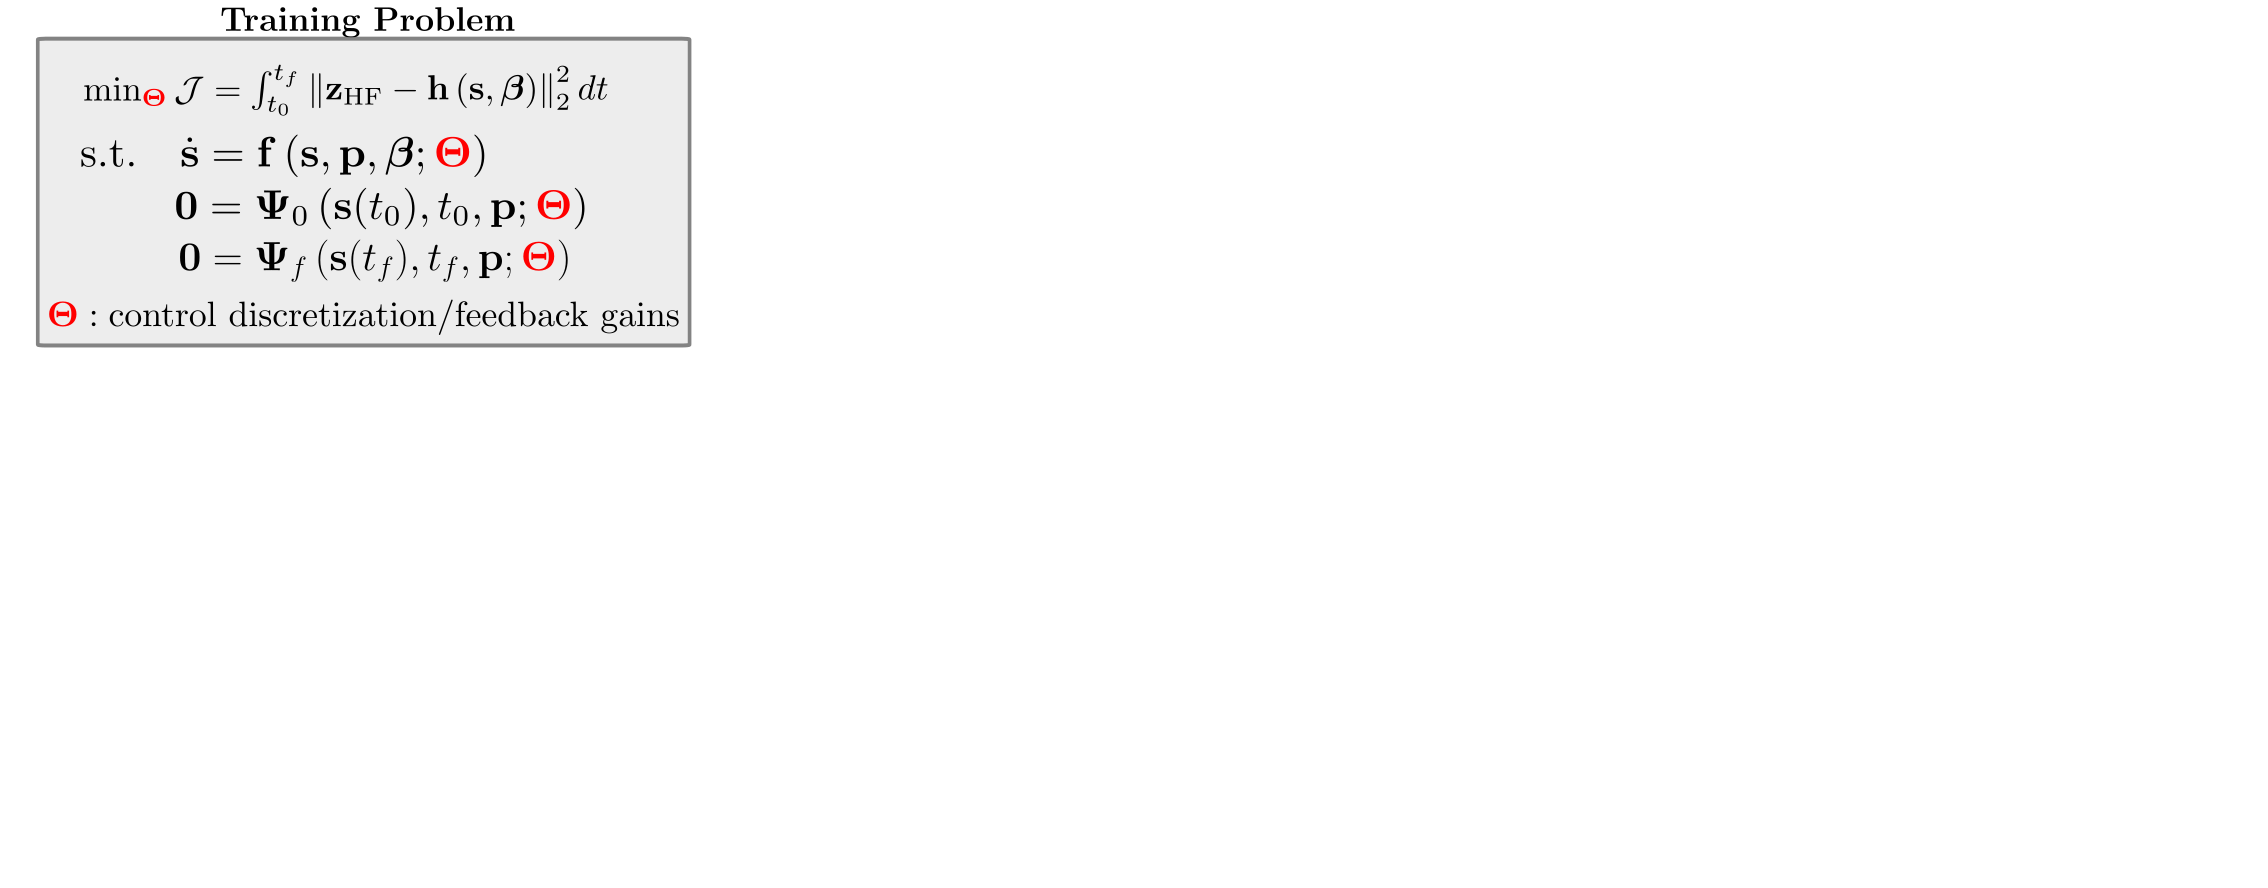
\includegraphics[width=0.95\textwidth]{../figs/ct/ct_overview_1.png}
        \end{figure}}
    \only<3>{
        \begin{figure}
            \centering
            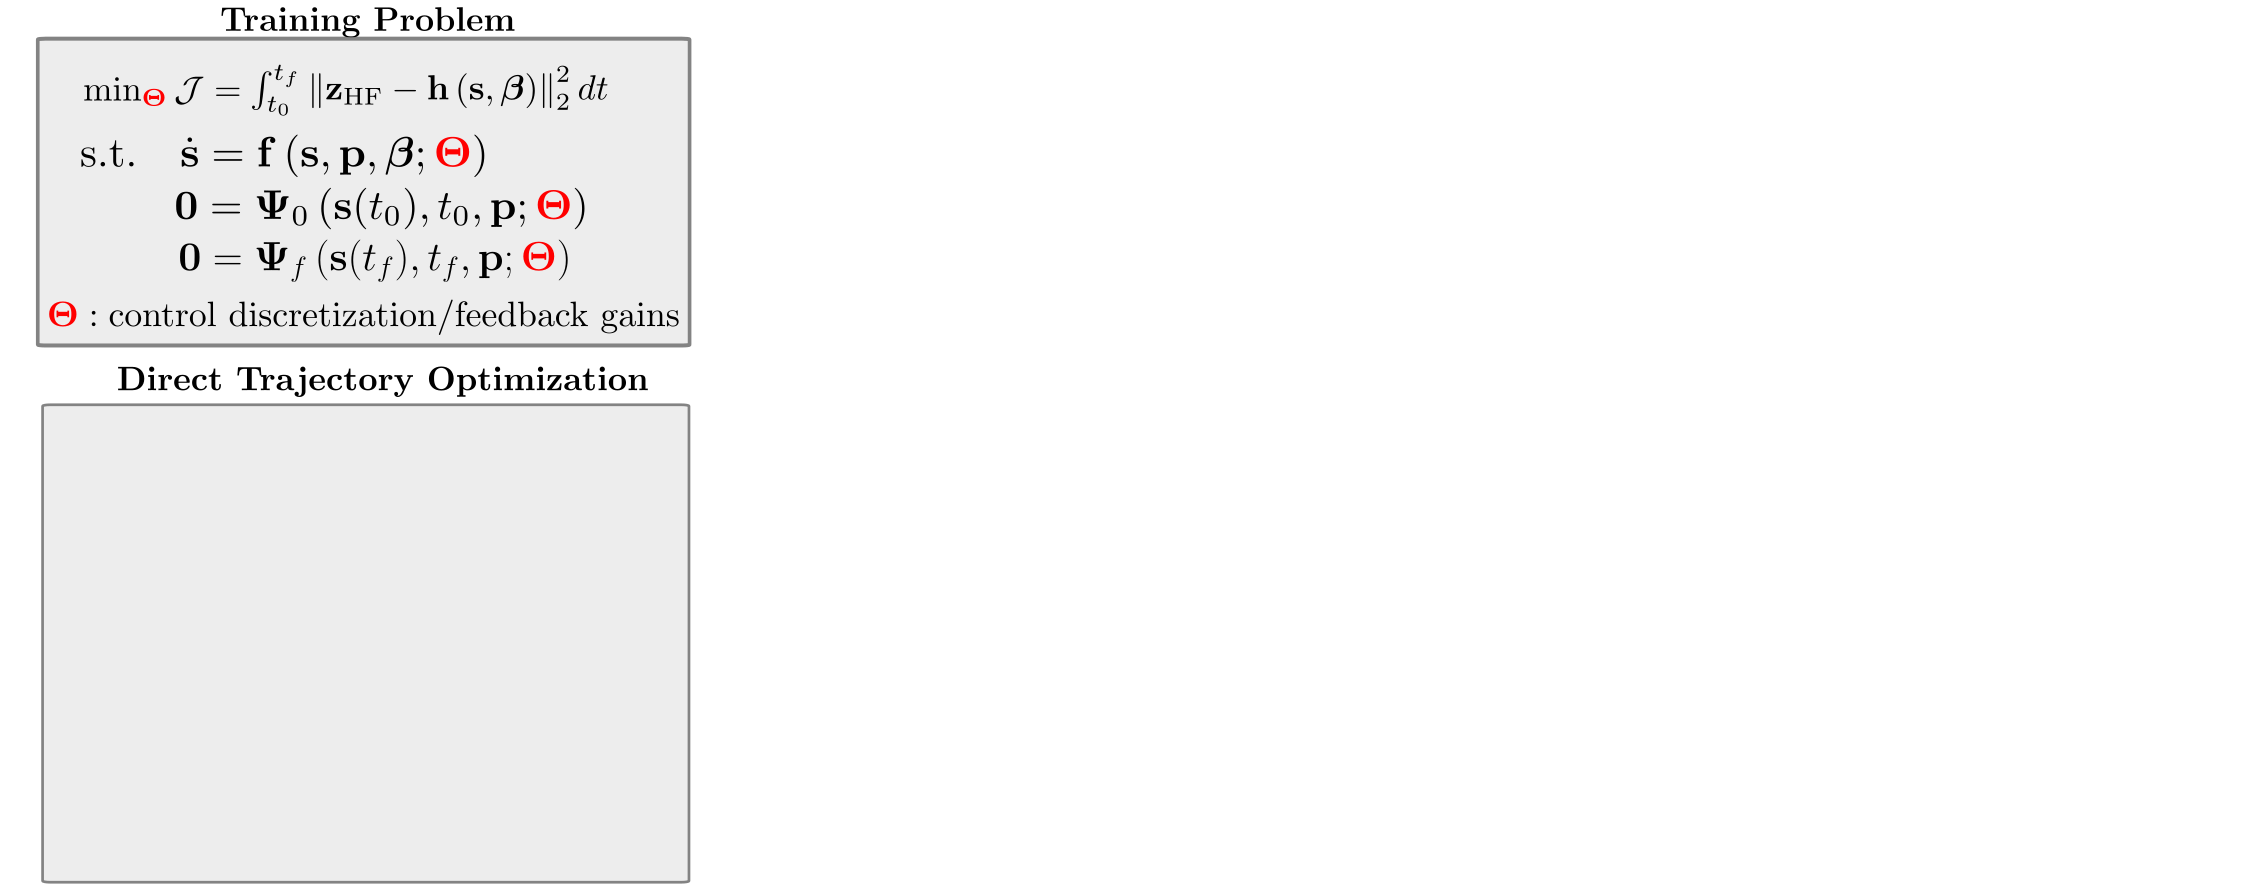
\includegraphics[width=0.95\textwidth]{../figs/ct/ct_overview_2.png}
        \end{figure}}
    \only<4>{
        \begin{figure}
            \centering
            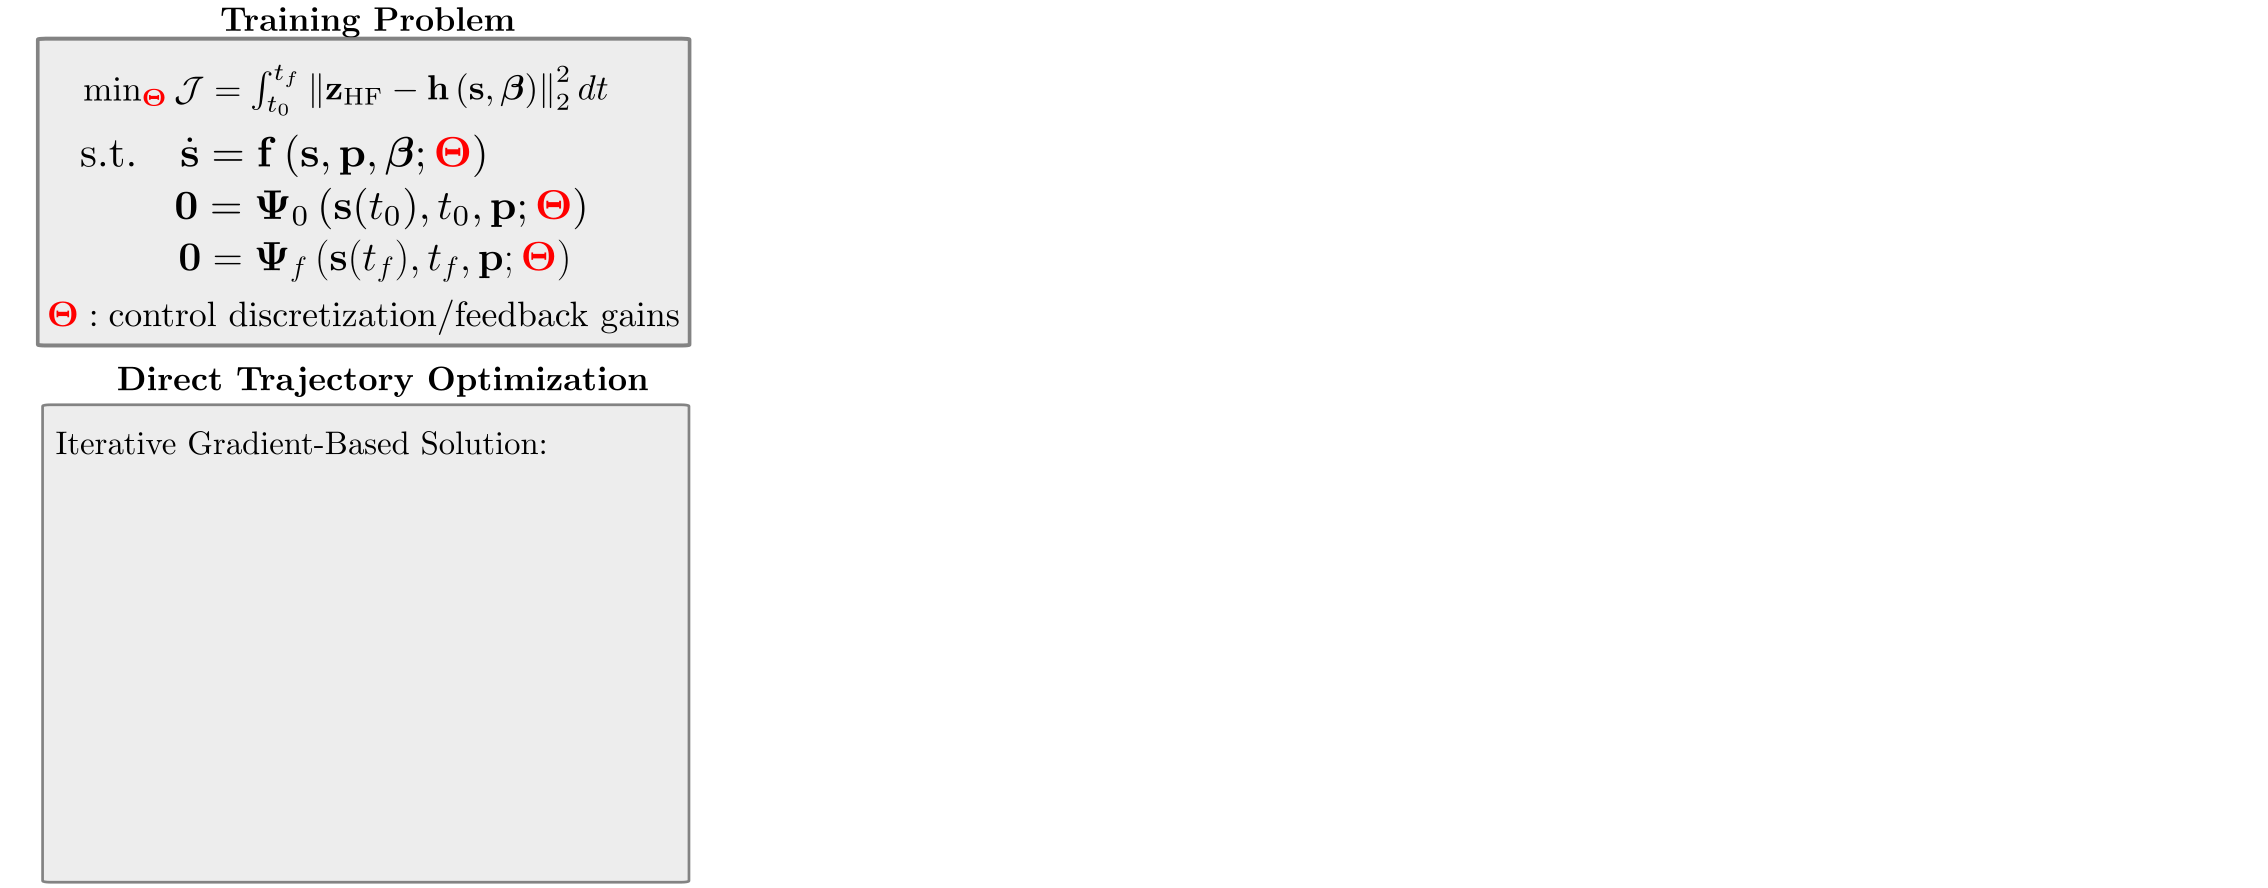
\includegraphics[width=0.95\textwidth]{../figs/ct/ct_overview_3.png}
        \end{figure}}
    \only<5>{
        \begin{figure}
            \centering
            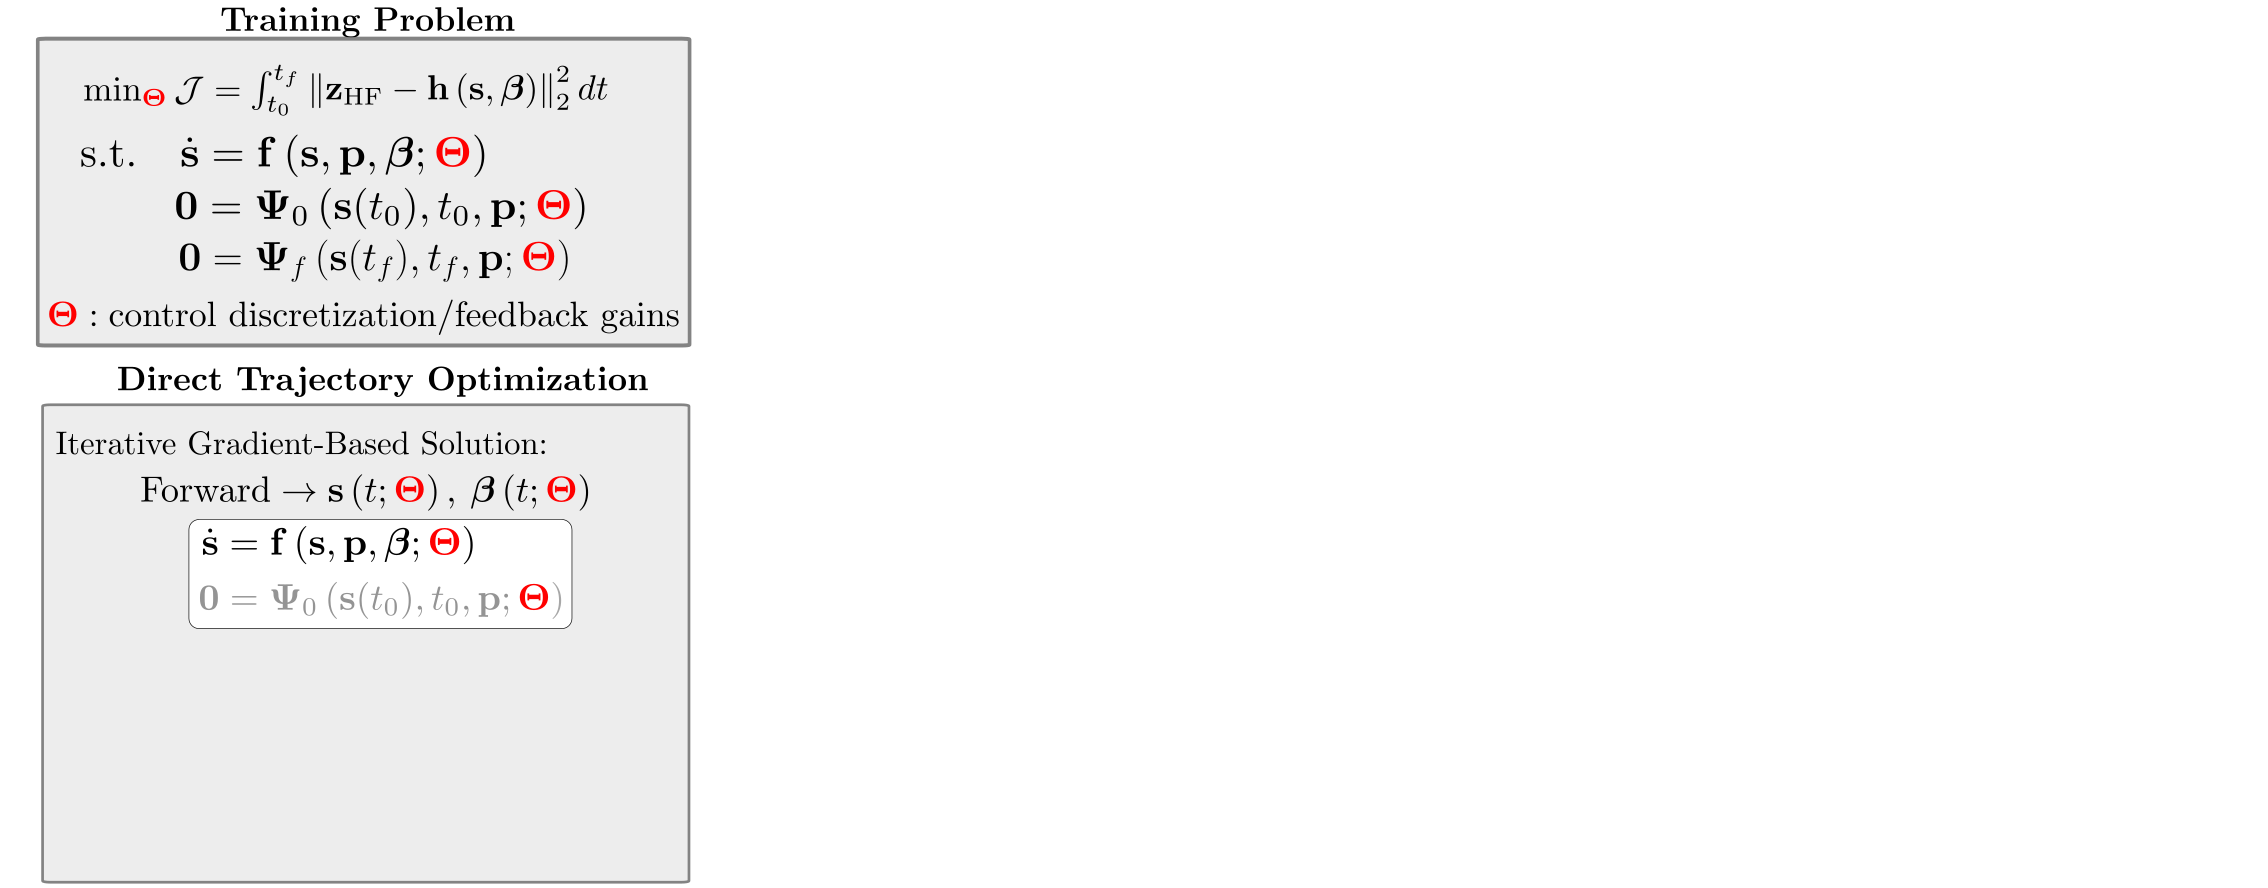
\includegraphics[width=0.95\textwidth]{../figs/ct/ct_overview_4.png}
        \end{figure}}
    \only<6>{
        \begin{figure}
            \centering
            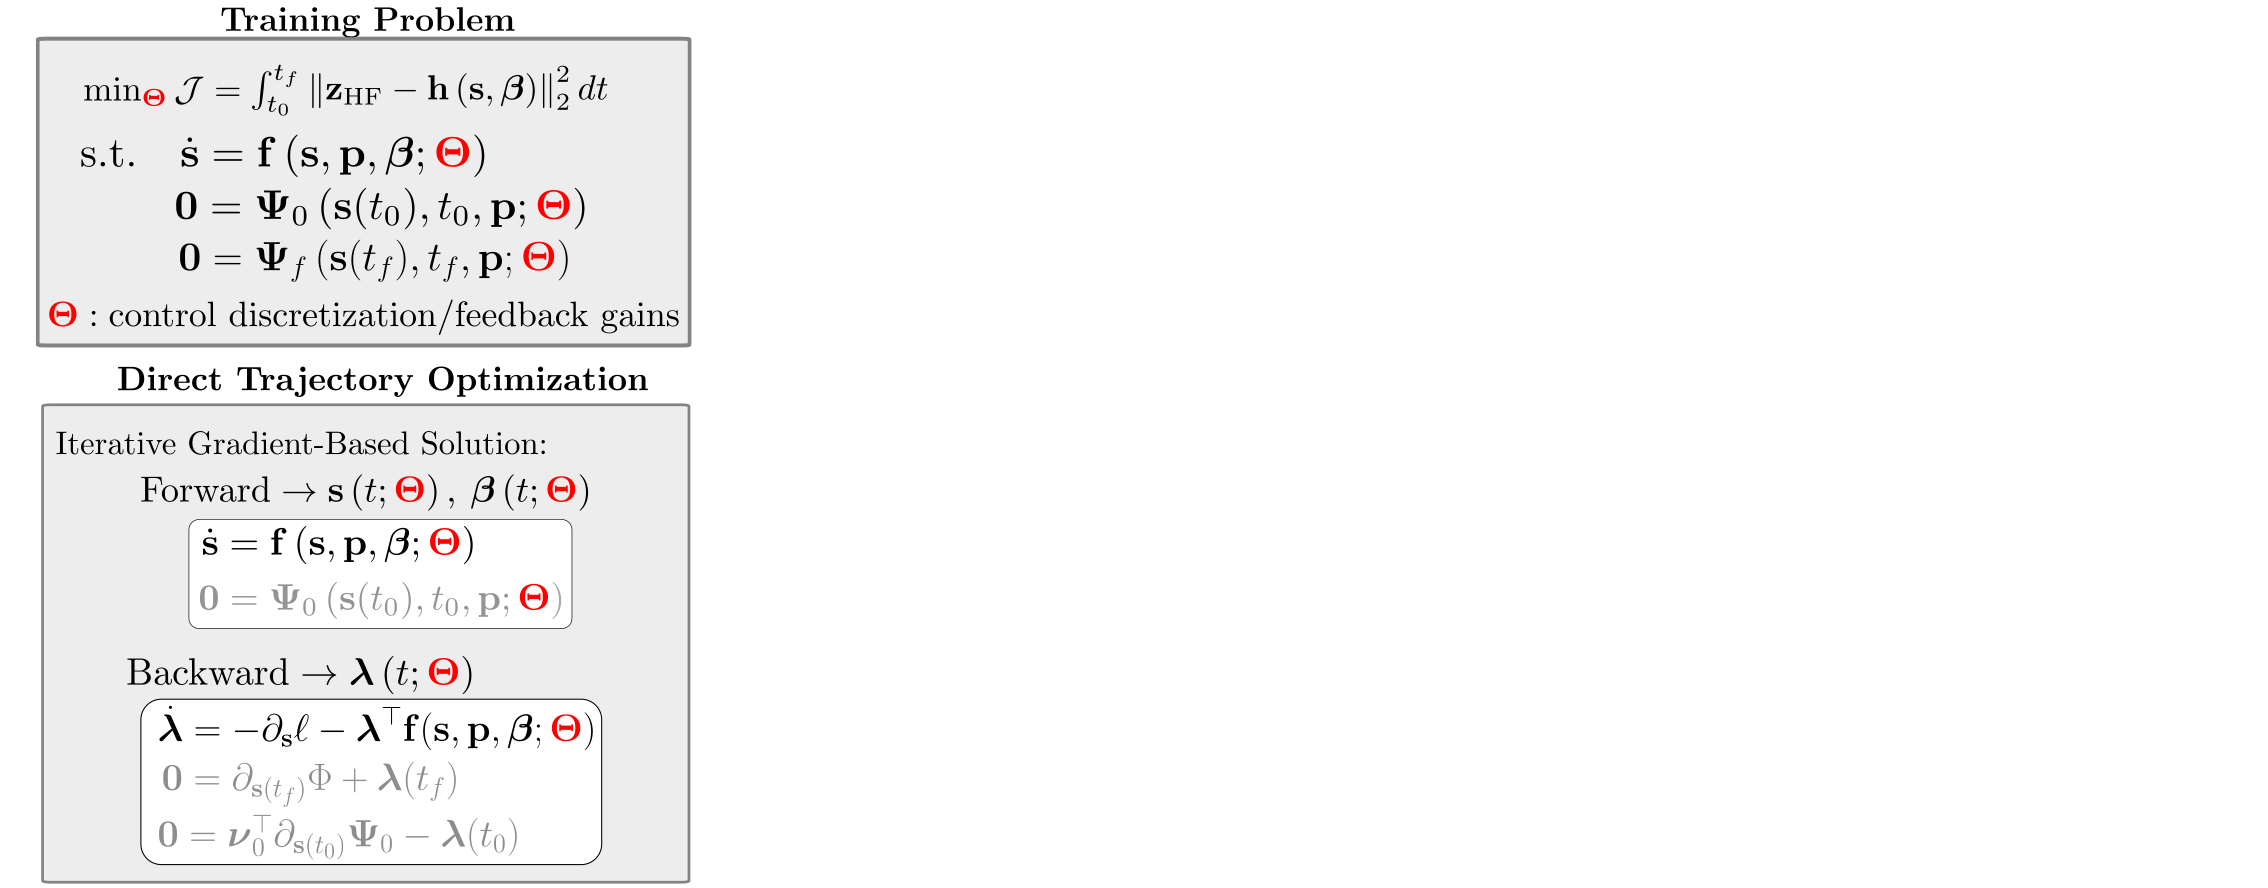
\includegraphics[width=0.95\textwidth]{../figs/ct/ct_overview_5.png}
        \end{figure}}
    \only<7>{
        \begin{figure}
            \centering
            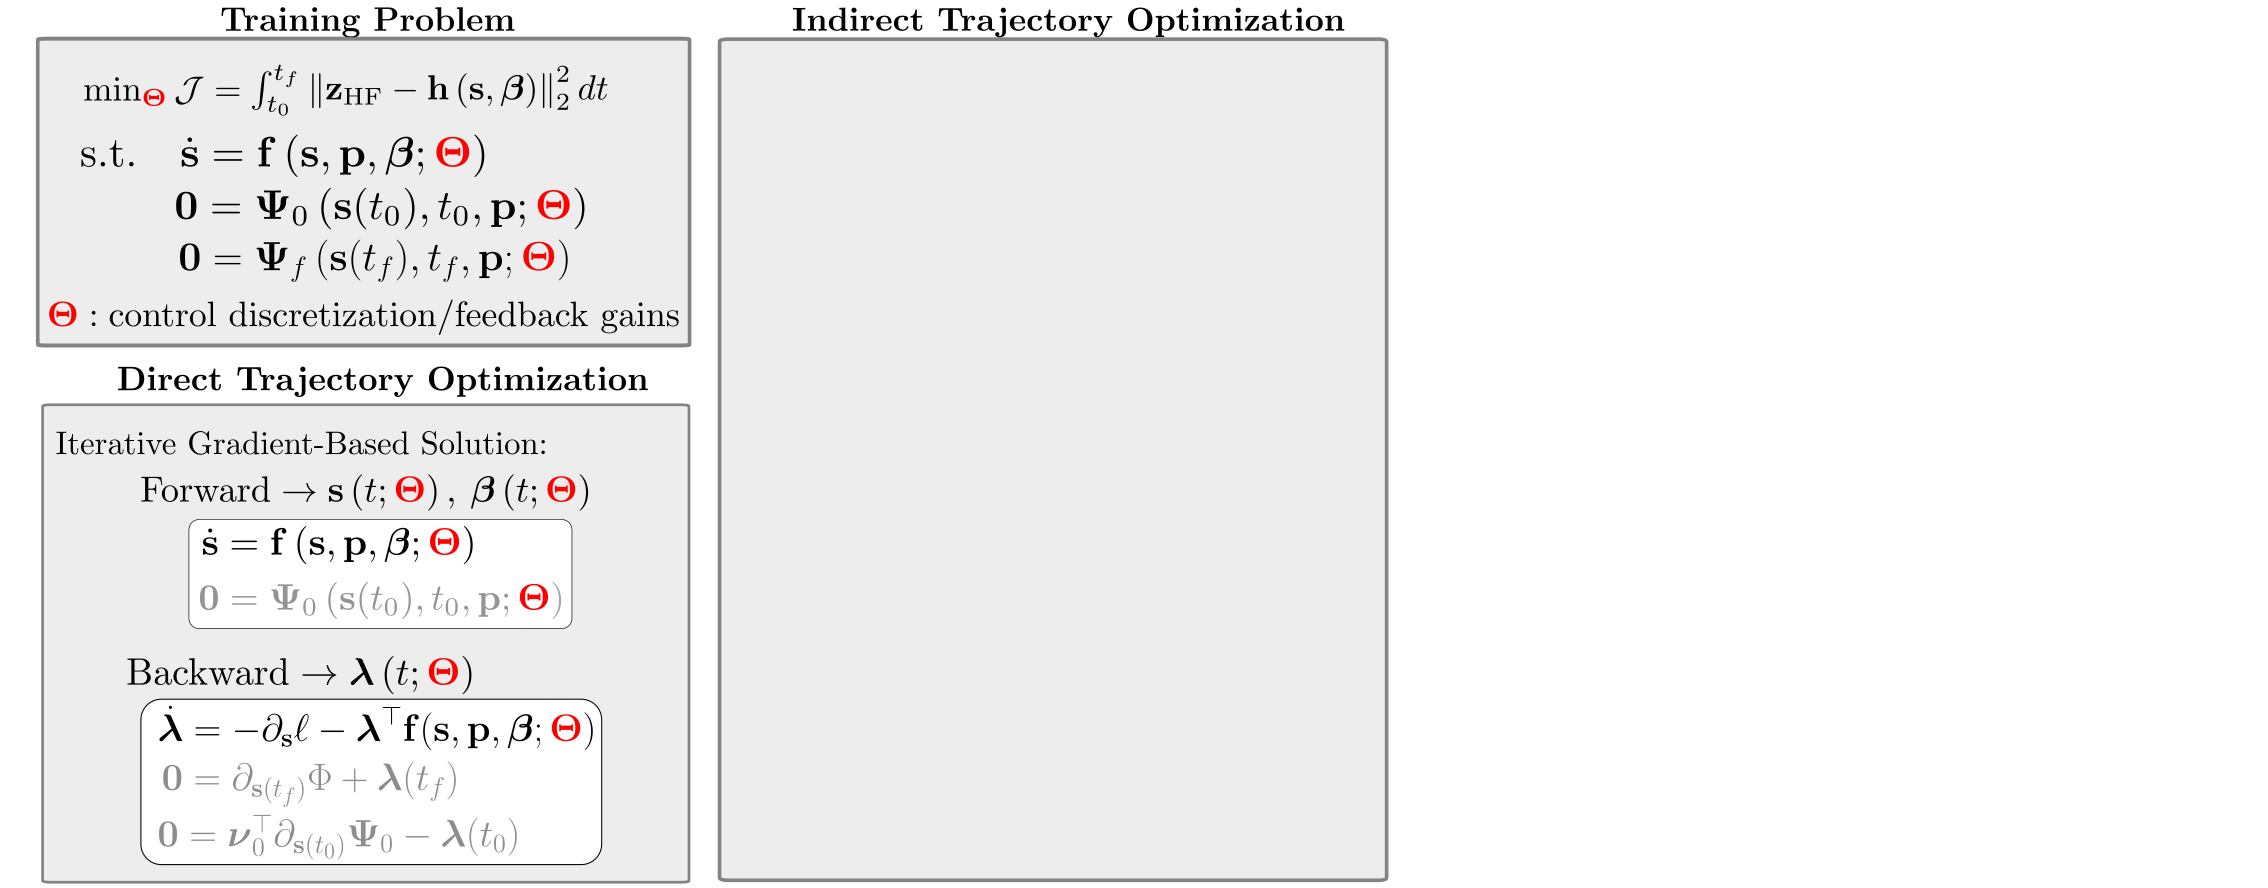
\includegraphics[width=0.95\textwidth]{../figs/ct/ct_overview_6.png}
        \end{figure}}
    \only<8>{
        \begin{figure}
            \centering
            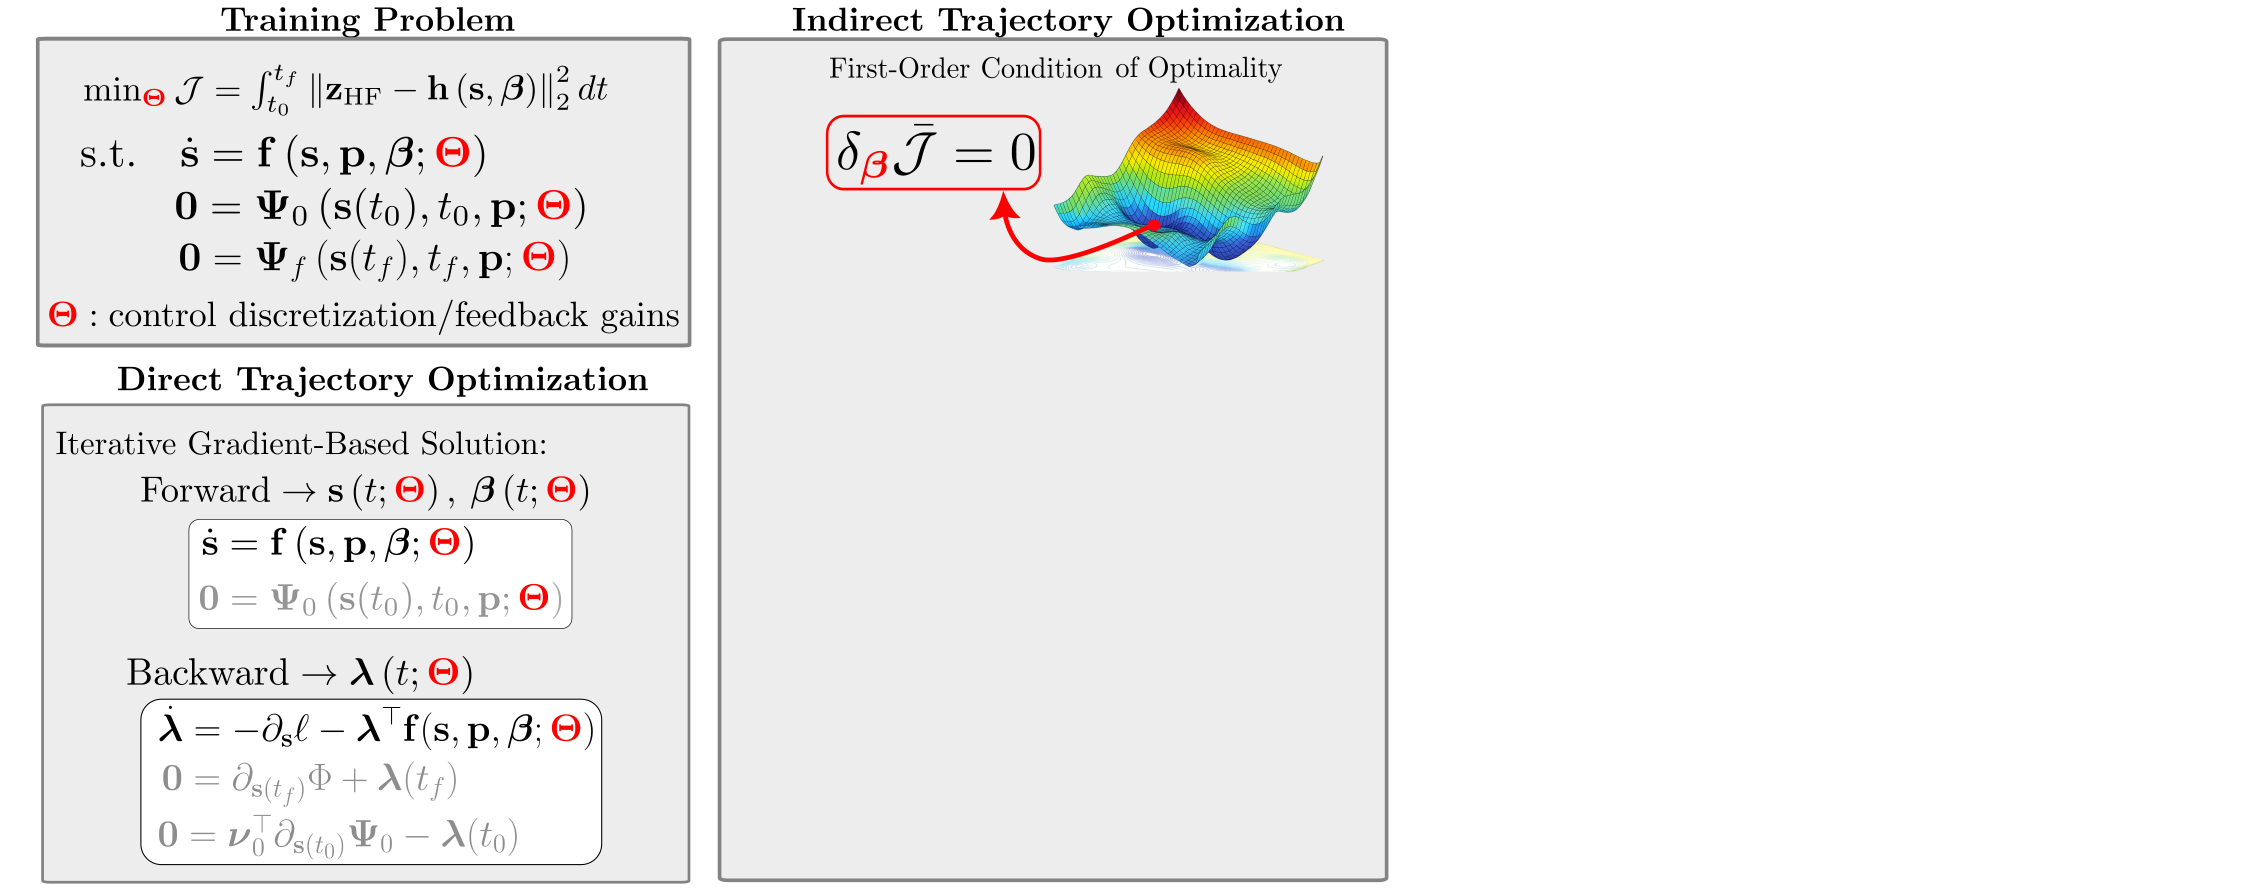
\includegraphics[width=0.95\textwidth]{../figs/ct/ct_overview_7.png}
        \end{figure}}
    \only<9>{
        \begin{figure}
            \centering
            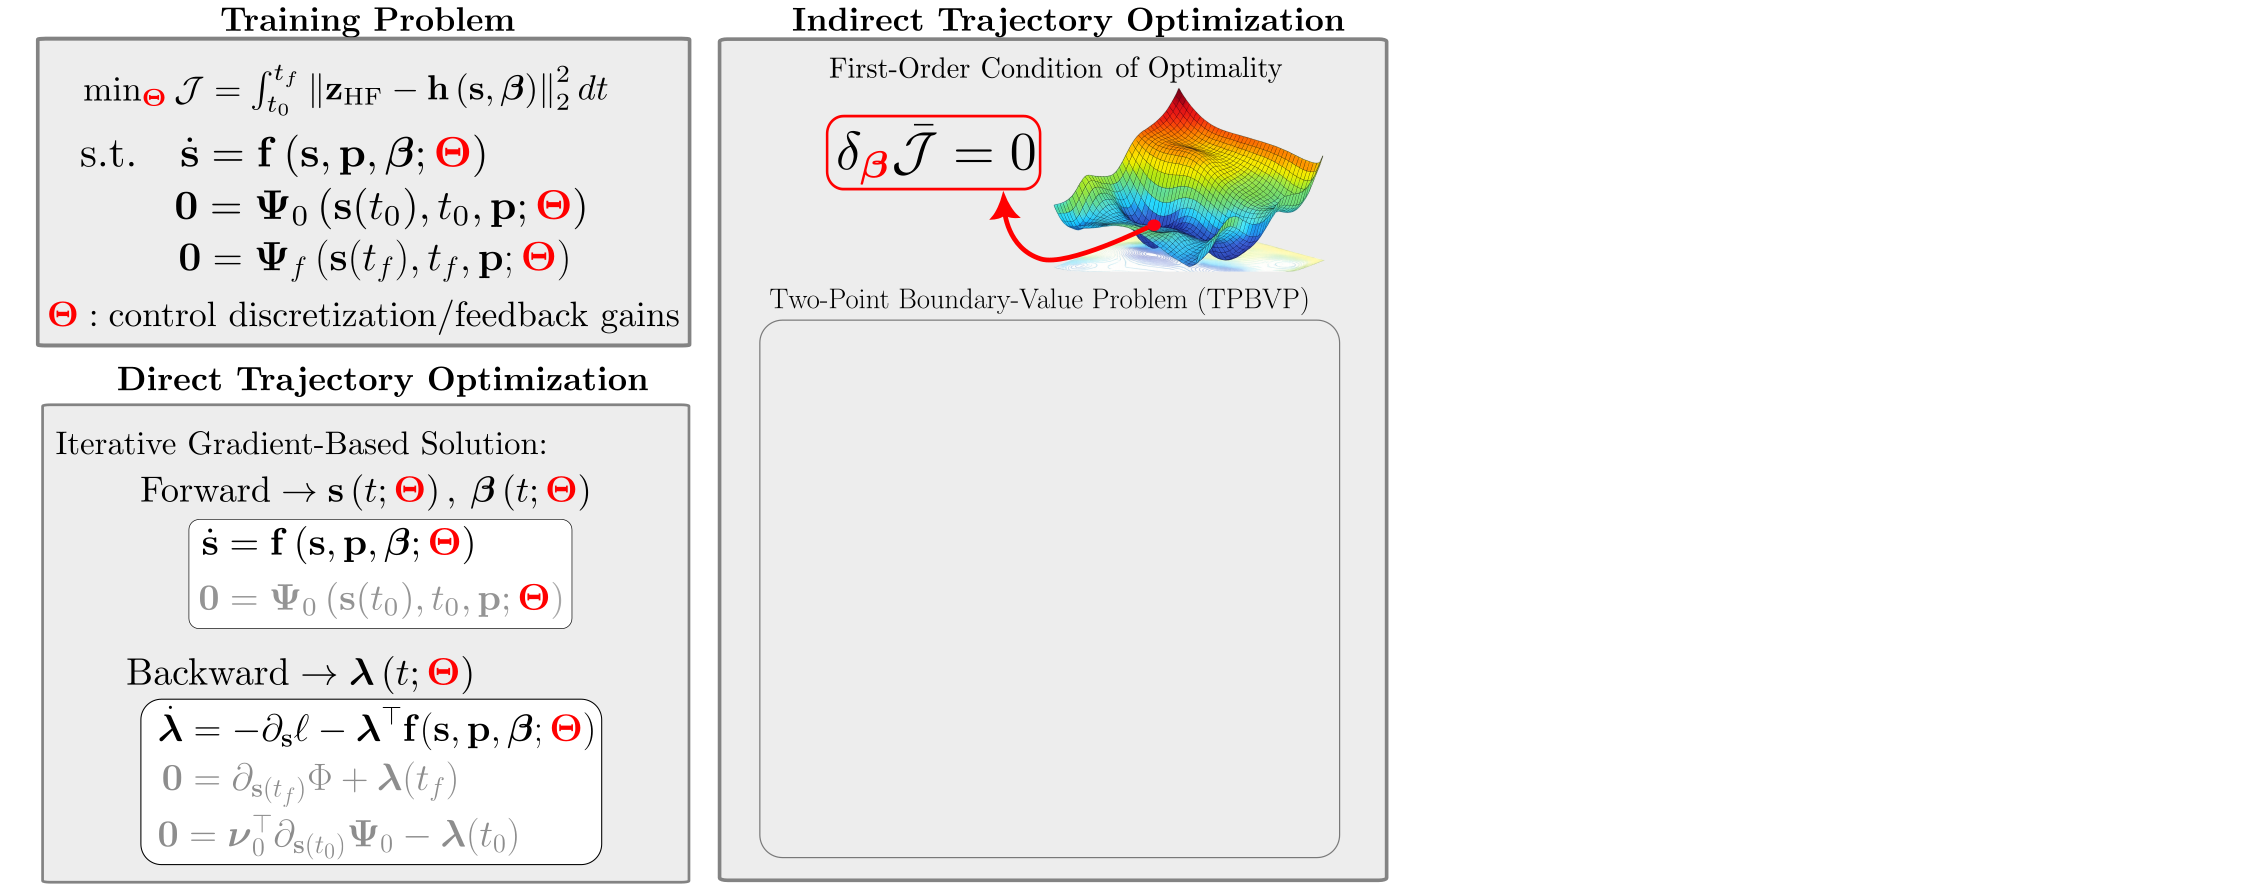
\includegraphics[width=0.95\textwidth]{../figs/ct/ct_overview_8.png}
        \end{figure}}
    \only<10>{
        \begin{figure}
            \centering
            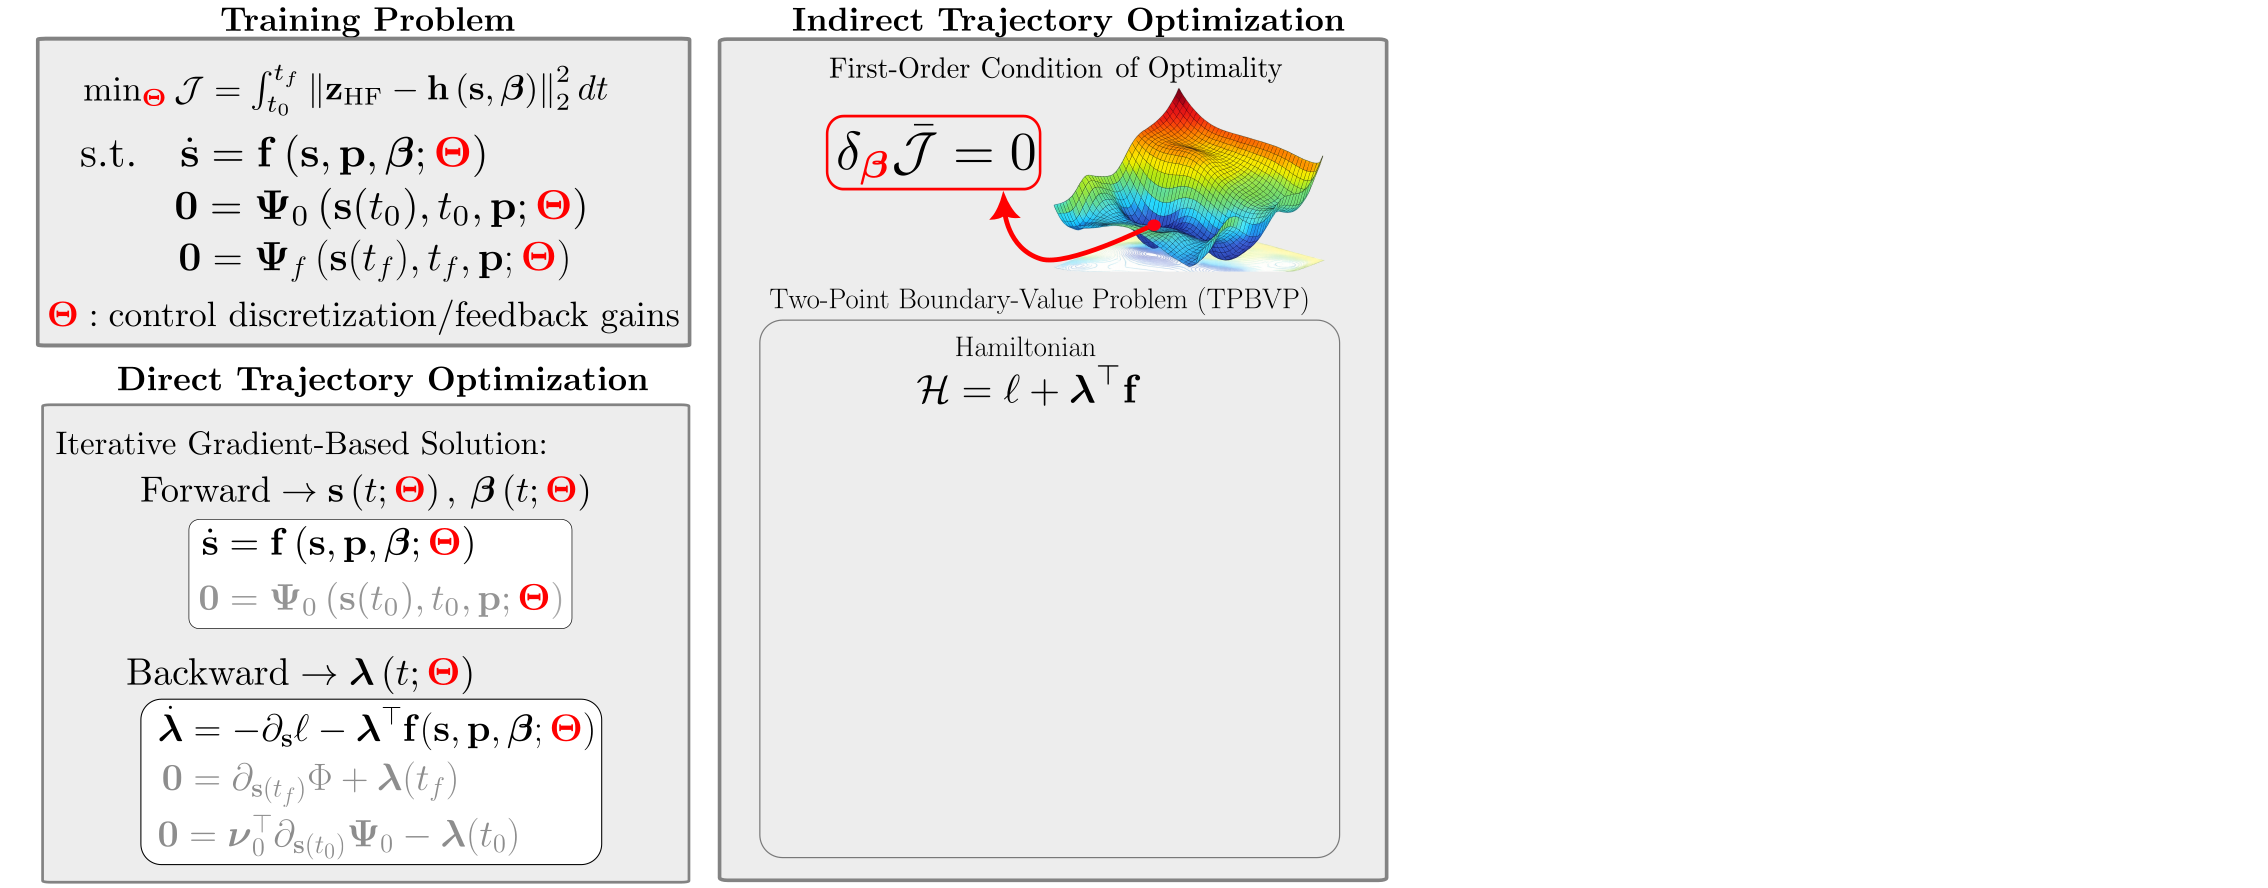
\includegraphics[width=0.95\textwidth]{../figs/ct/ct_overview_9.png}
        \end{figure}}
    \only<11>{
        \begin{figure}
            \centering
            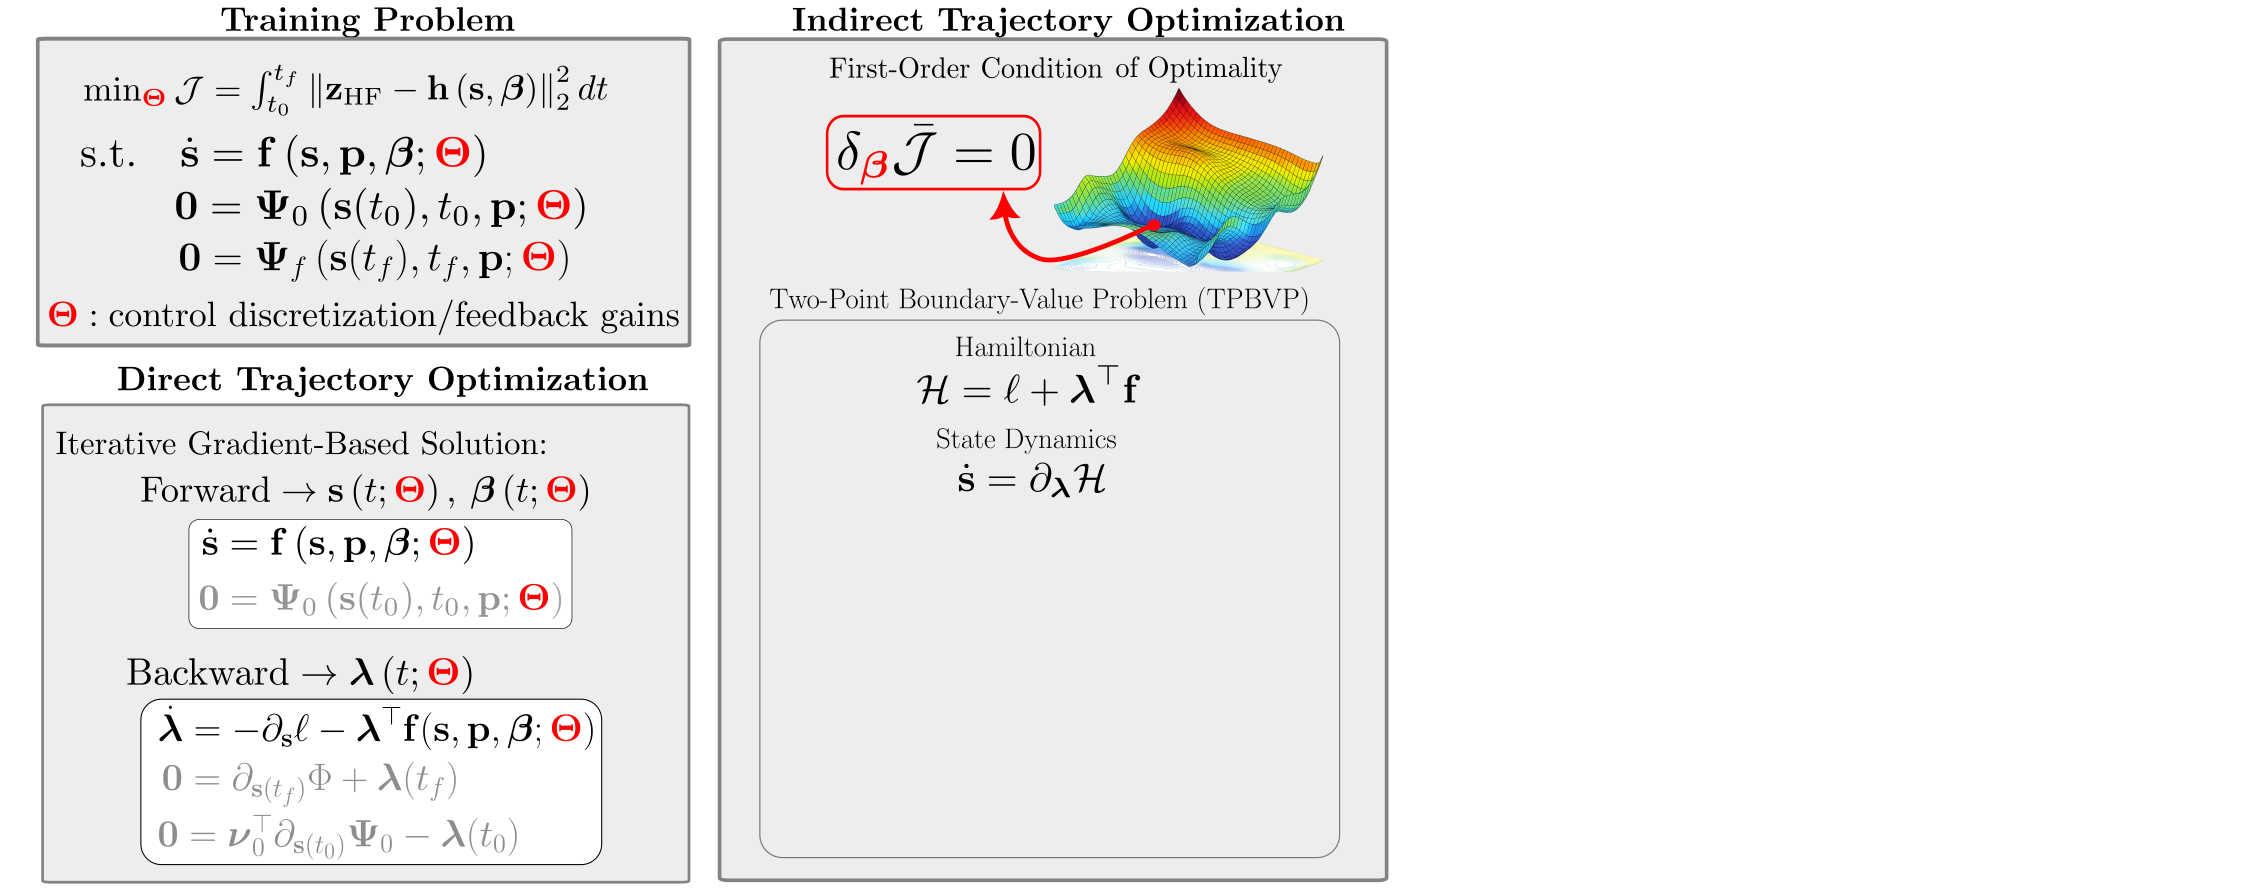
\includegraphics[width=0.95\textwidth]{../figs/ct/ct_overview_10.png}
        \end{figure}}
    \only<12>{
        \begin{figure}
            \centering
            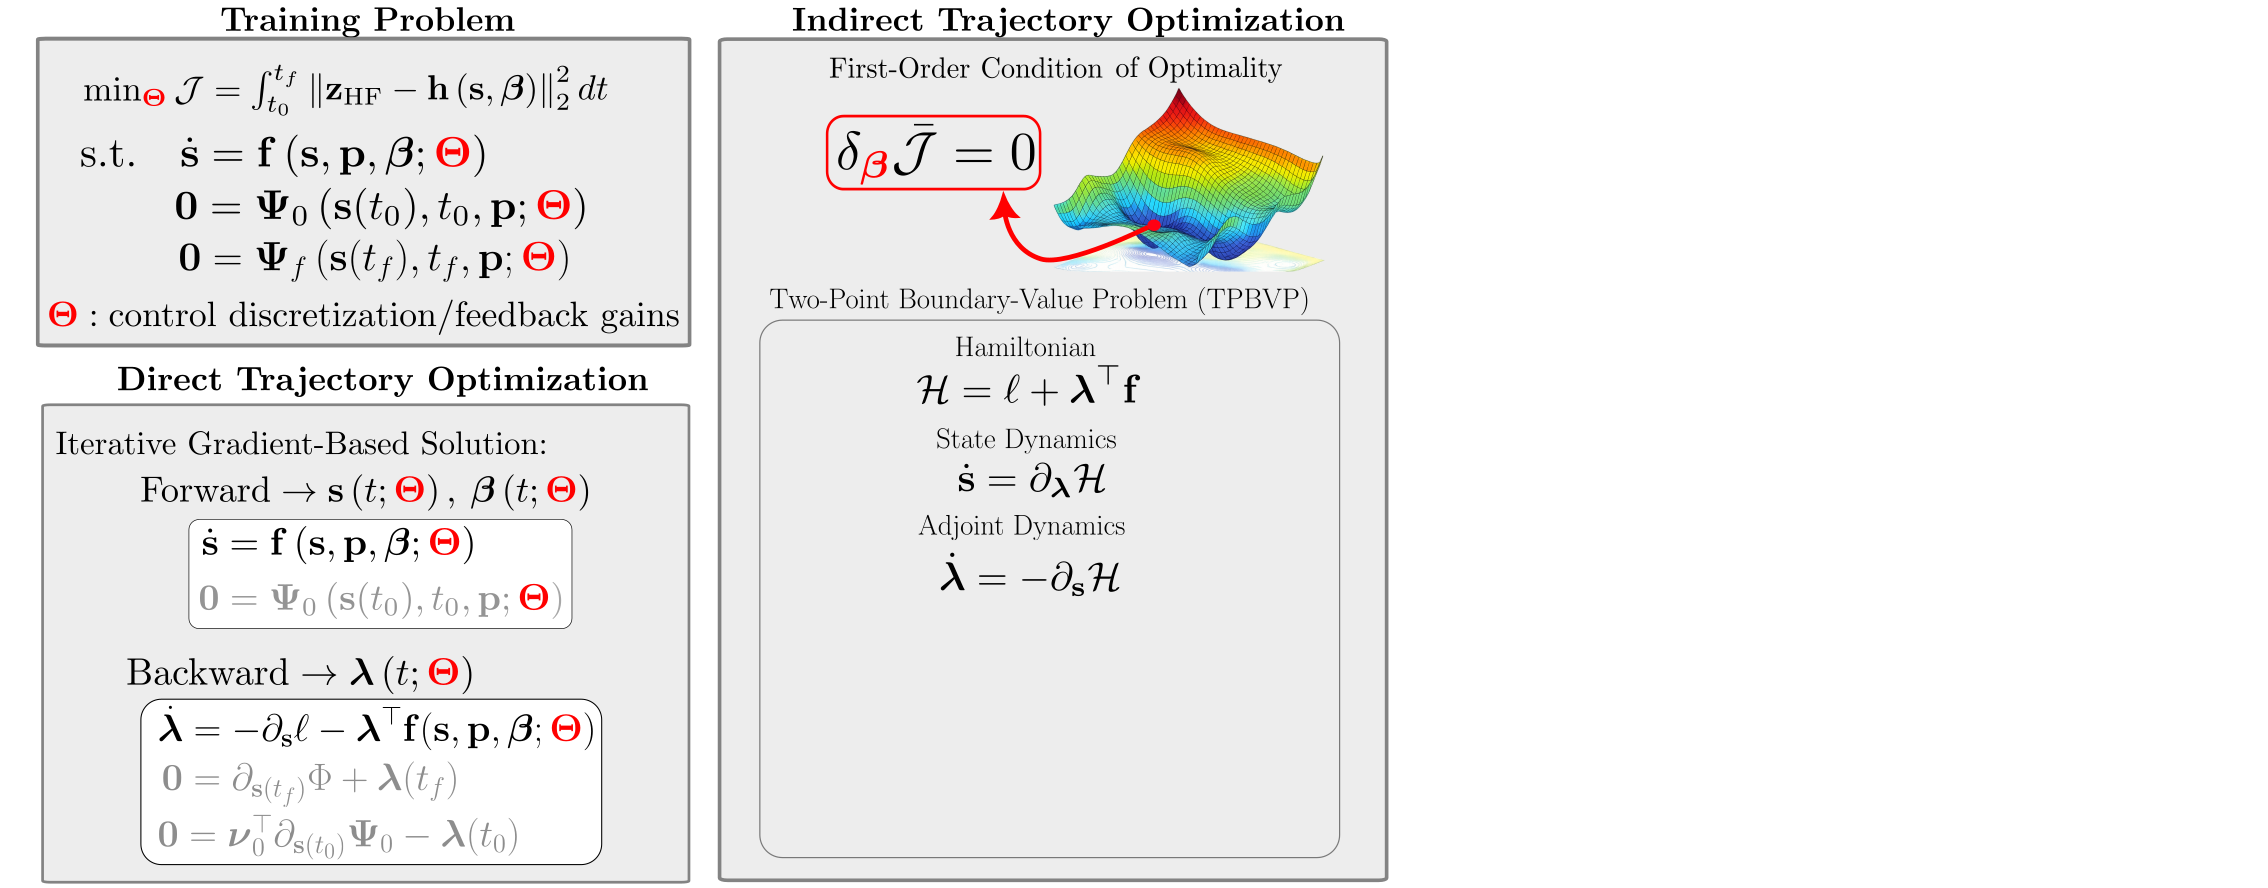
\includegraphics[width=0.95\textwidth]{../figs/ct/ct_overview_11.png}
        \end{figure}}
    \only<13>{
        \begin{figure}
            \centering
            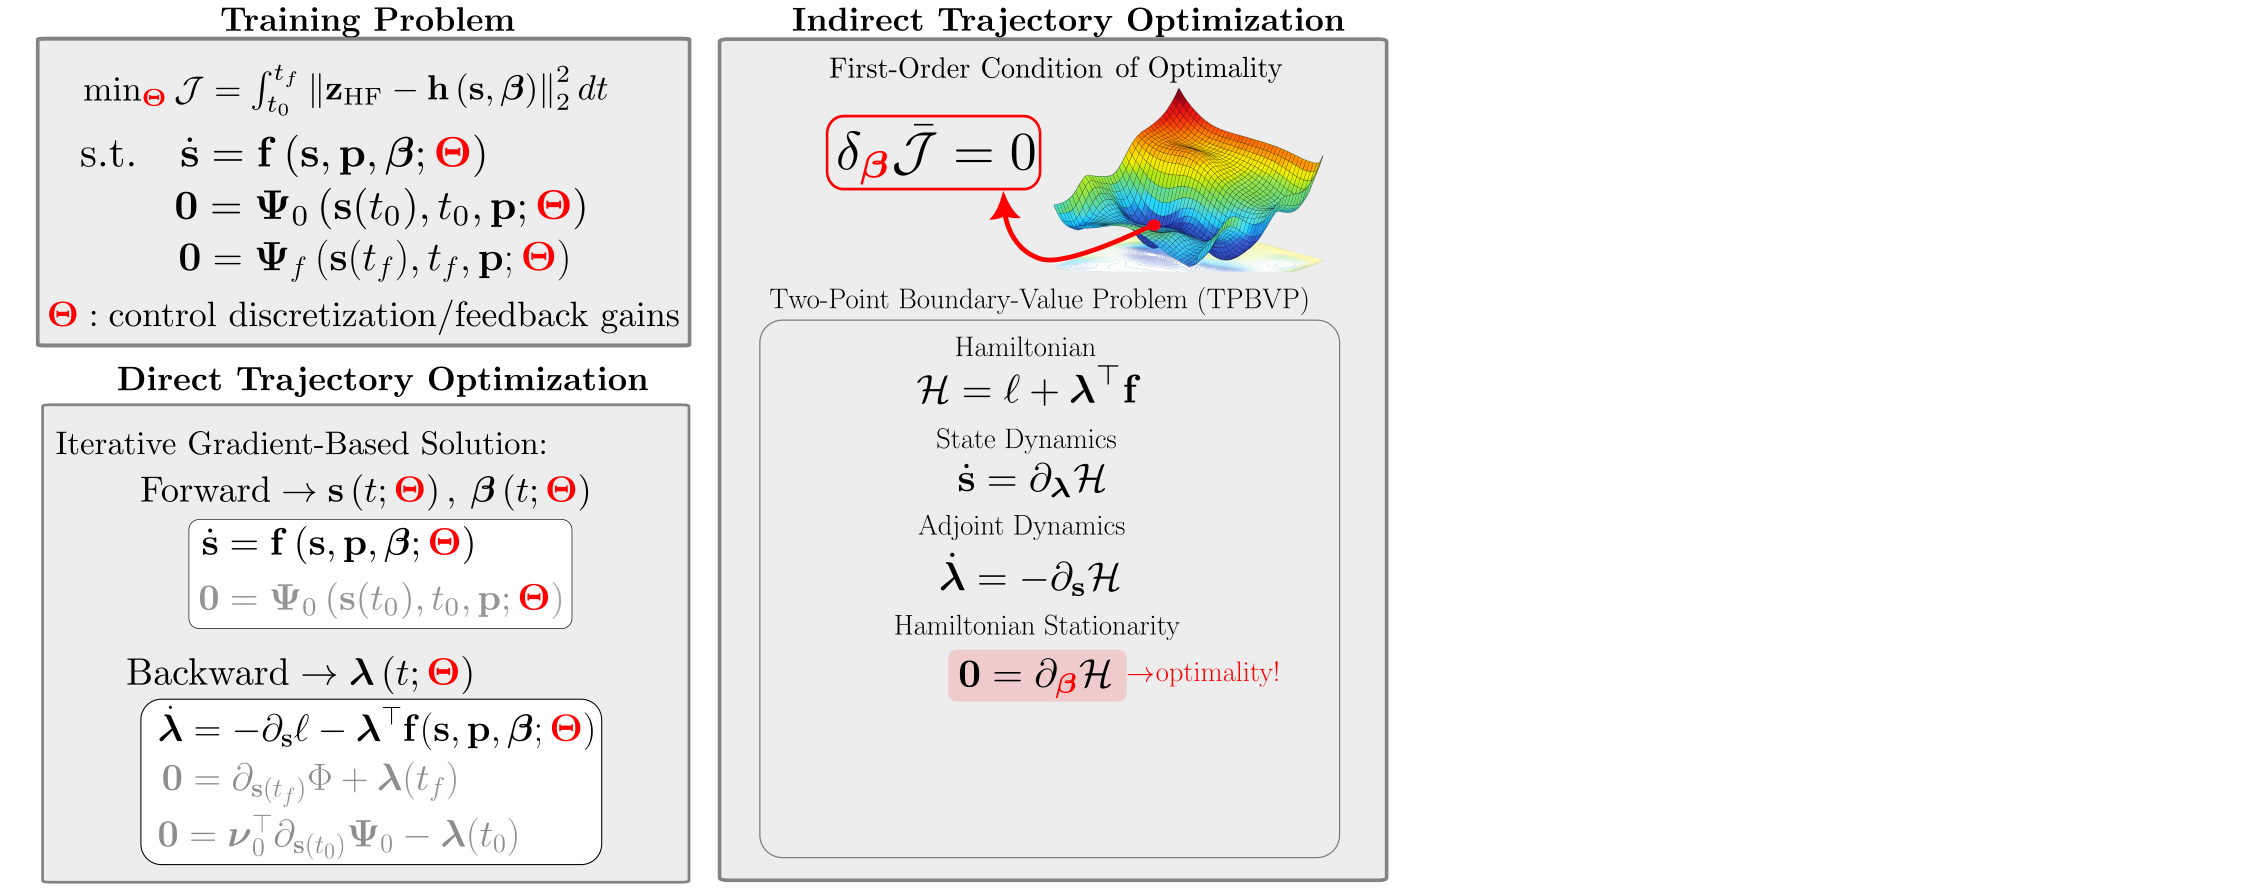
\includegraphics[width=0.95\textwidth]{../figs/ct/ct_overview_12.png}
        \end{figure}}
    \only<14>{
        \begin{figure}
            \centering
            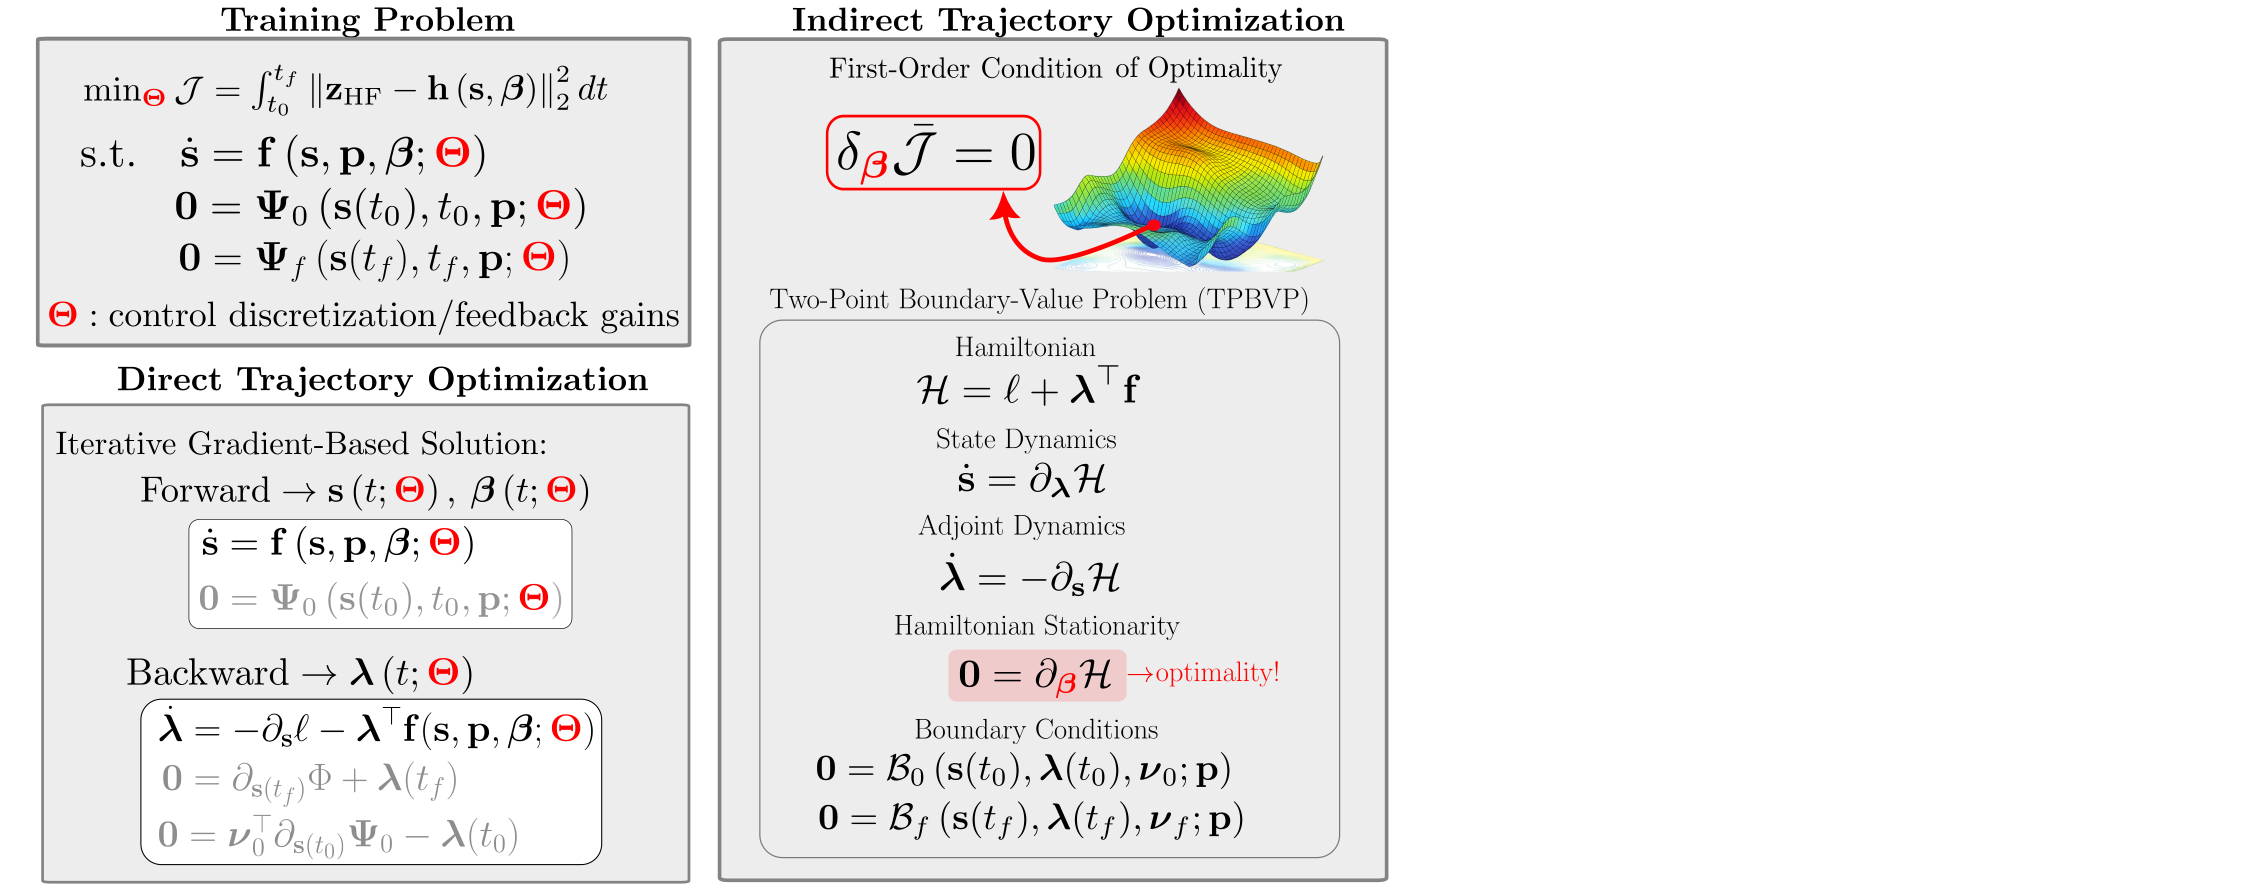
\includegraphics[width=0.95\textwidth]{../figs/ct/ct_overview_13.png}
        \end{figure}}
    \only<15>{
        \begin{figure}
            \centering
            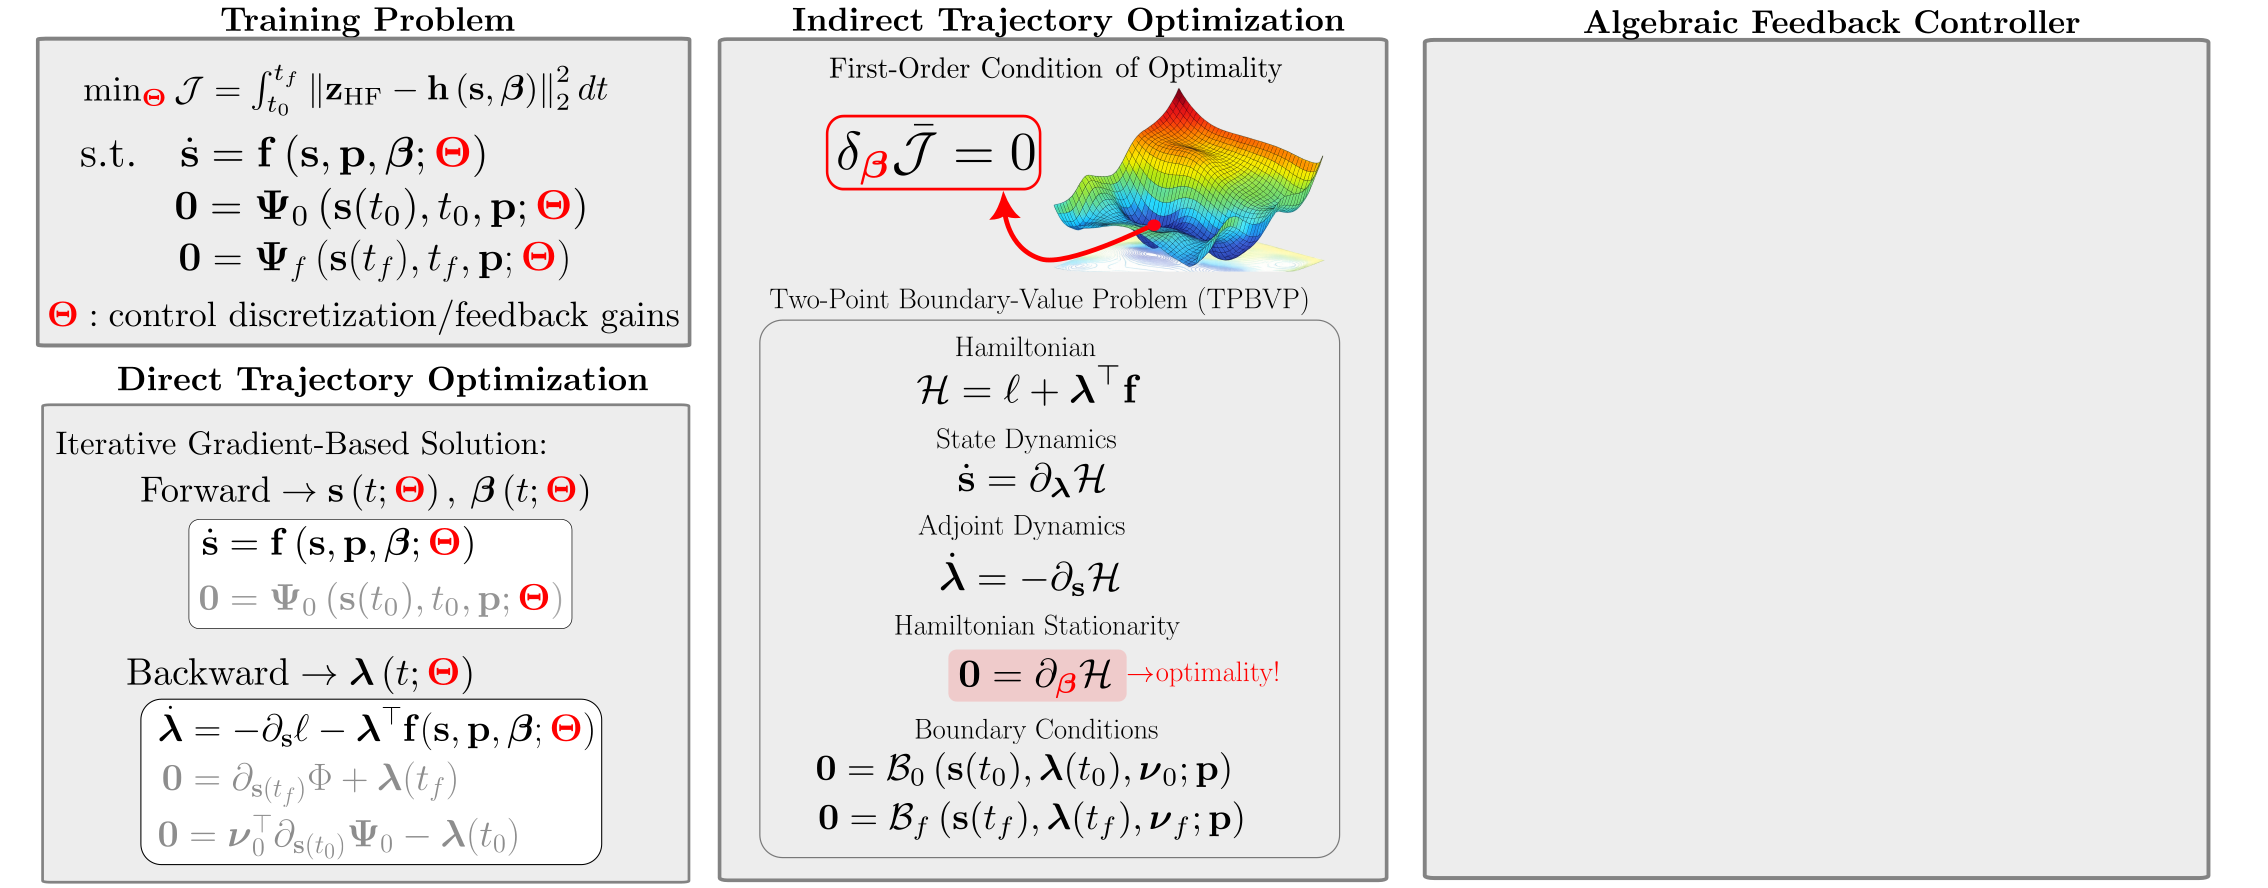
\includegraphics[width=0.95\textwidth]{../figs/ct/ct_overview_14.png}
        \end{figure}}
    \only<16>{
        \begin{figure}
            \centering
            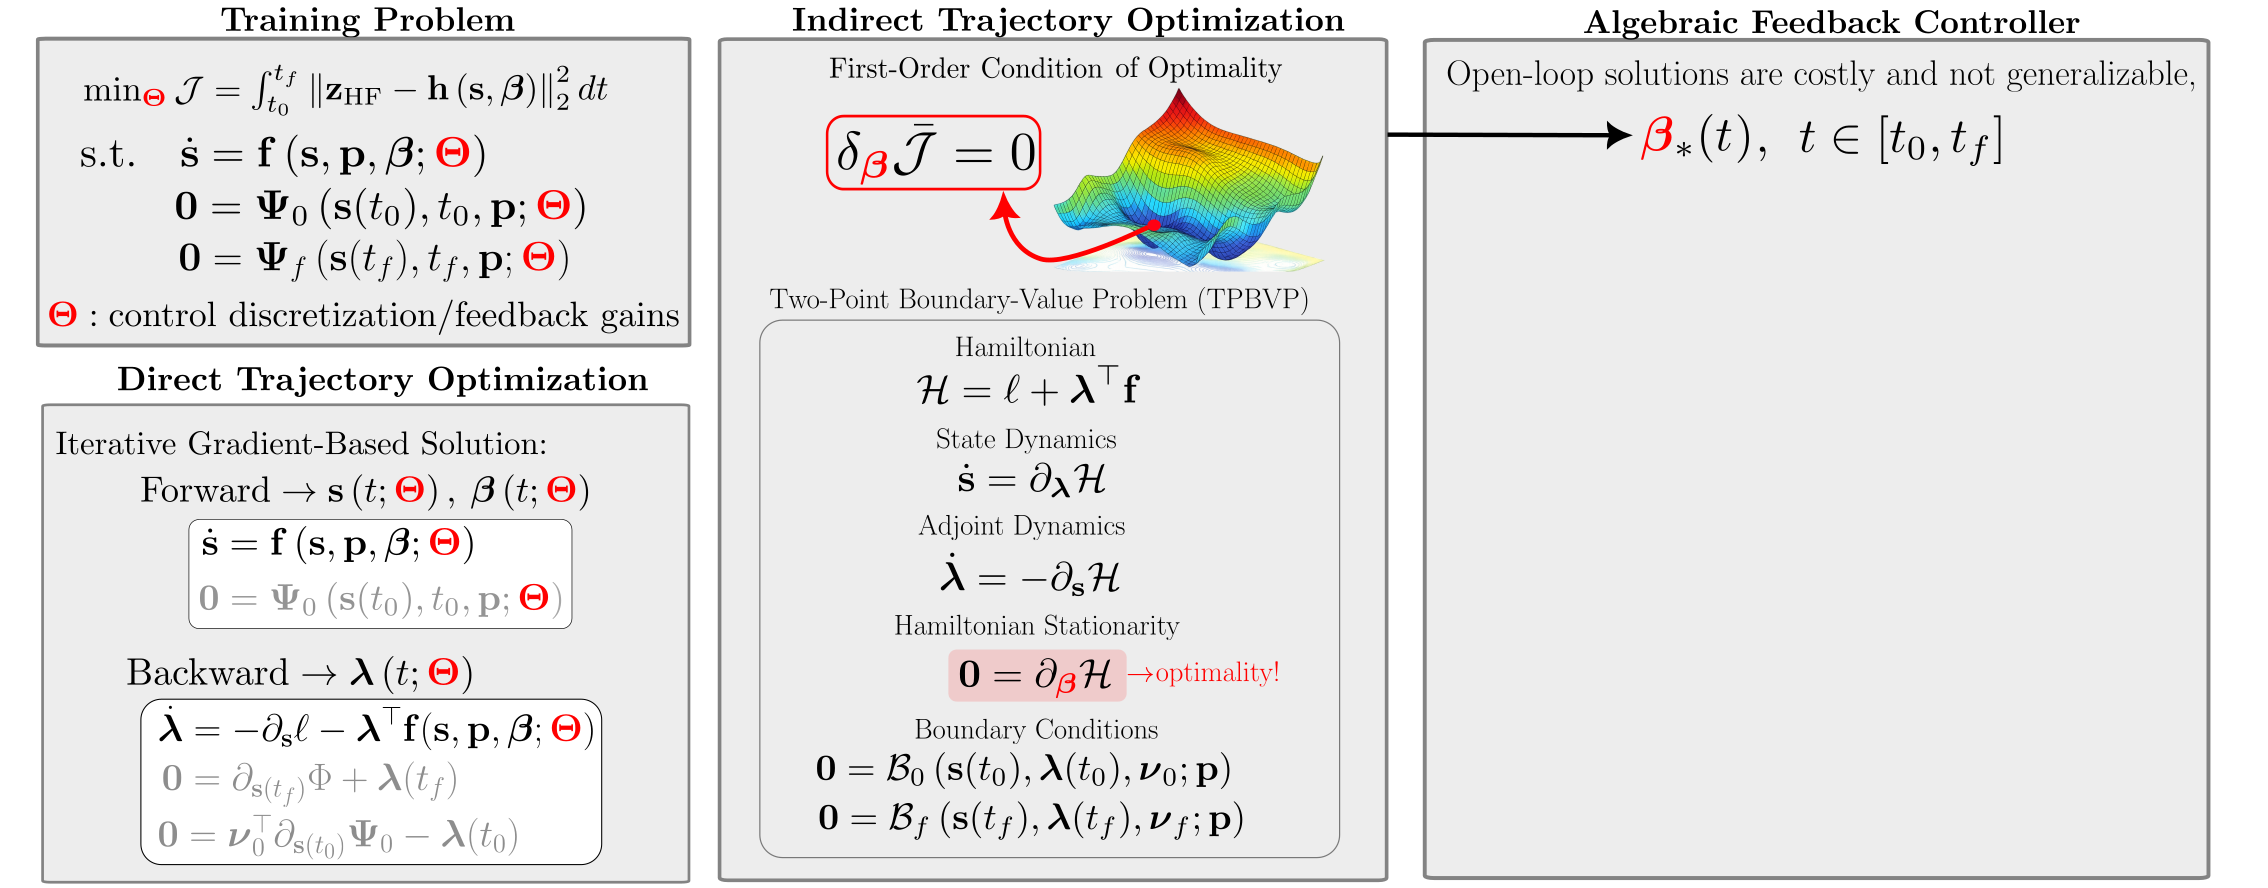
\includegraphics[width=0.95\textwidth]{../figs/ct/ct_overview_15.png}
        \end{figure}}
    \only<17>{
        \begin{figure}
            \centering
            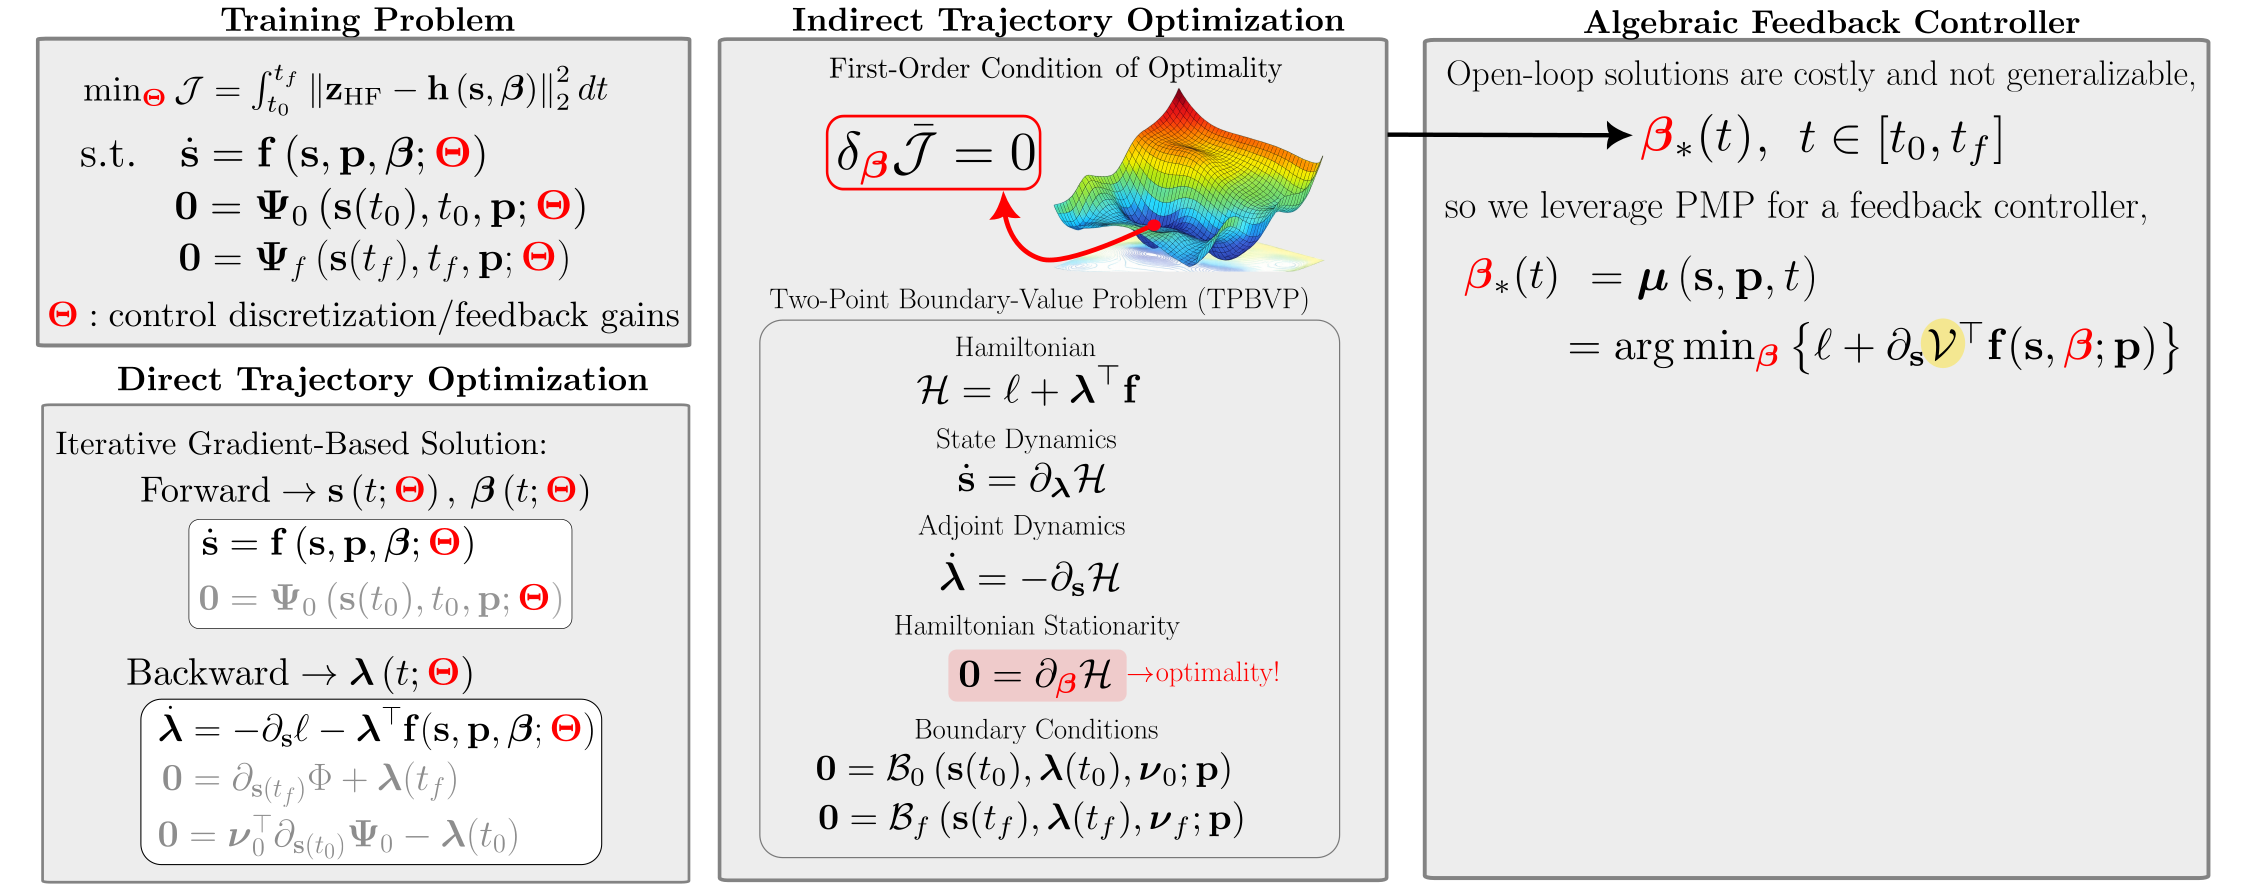
\includegraphics[width=0.95\textwidth]{../figs/ct/ct_overview_16.png}
        \end{figure}}
    \only<18>{
        \begin{figure}
            \centering
            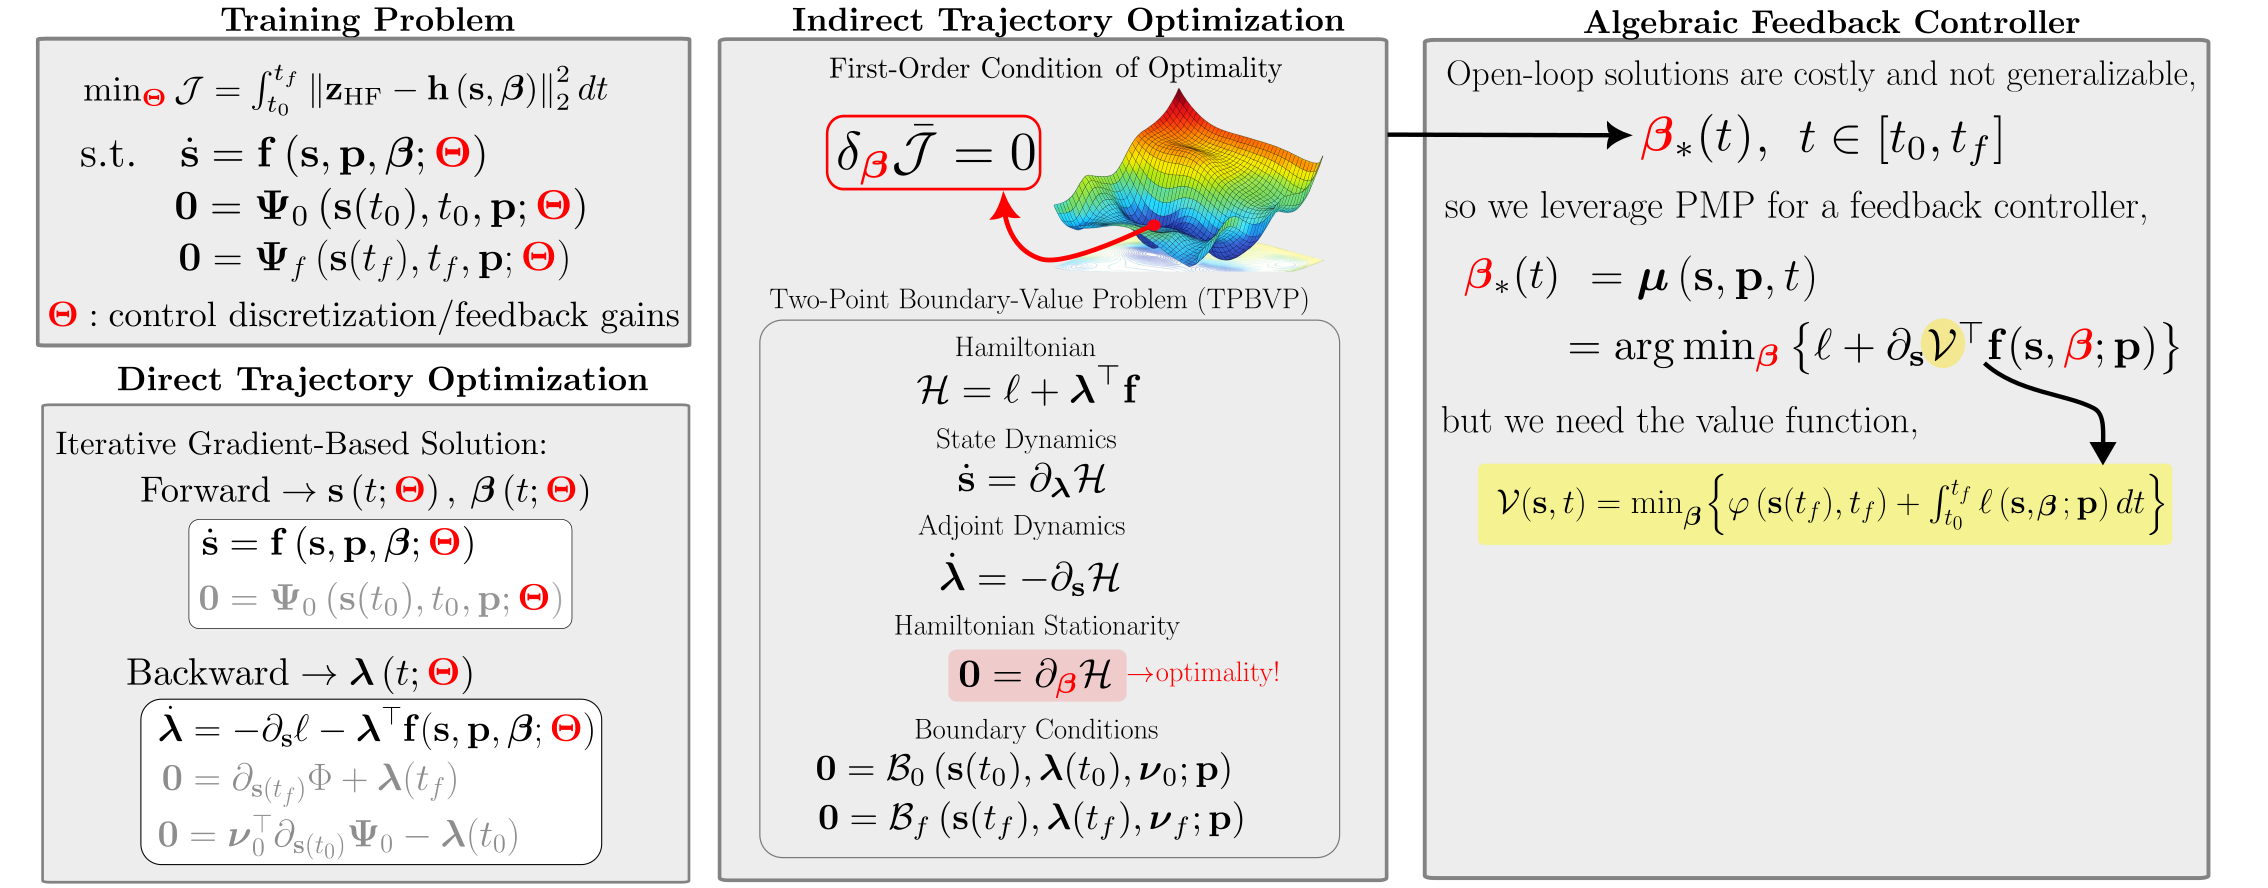
\includegraphics[width=0.95\textwidth]{../figs/ct/ct_overview_17.png}
        \end{figure}}
    \only<19>{
        \begin{figure}
            \centering
            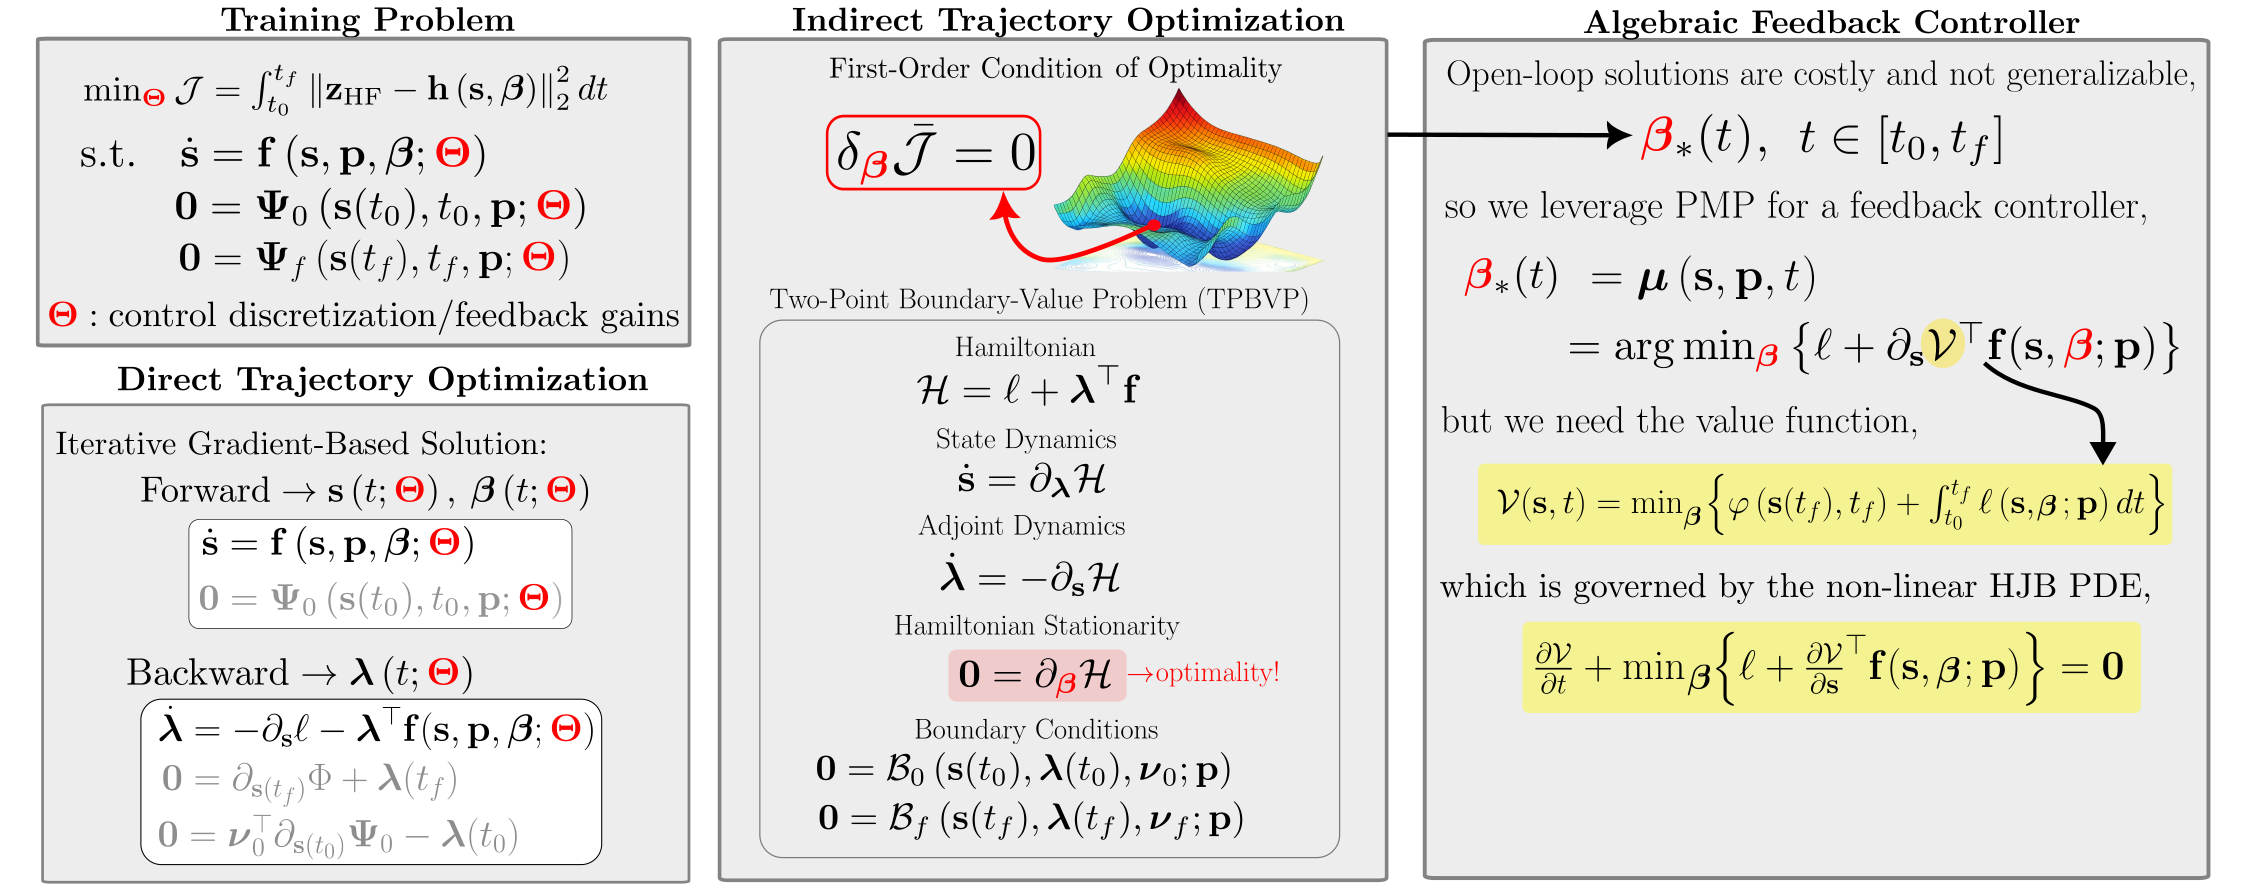
\includegraphics[width=0.95\textwidth]{../figs/ct/ct_overview_18.png}
        \end{figure}}
    \only<20>{
        \begin{figure}
            \centering
            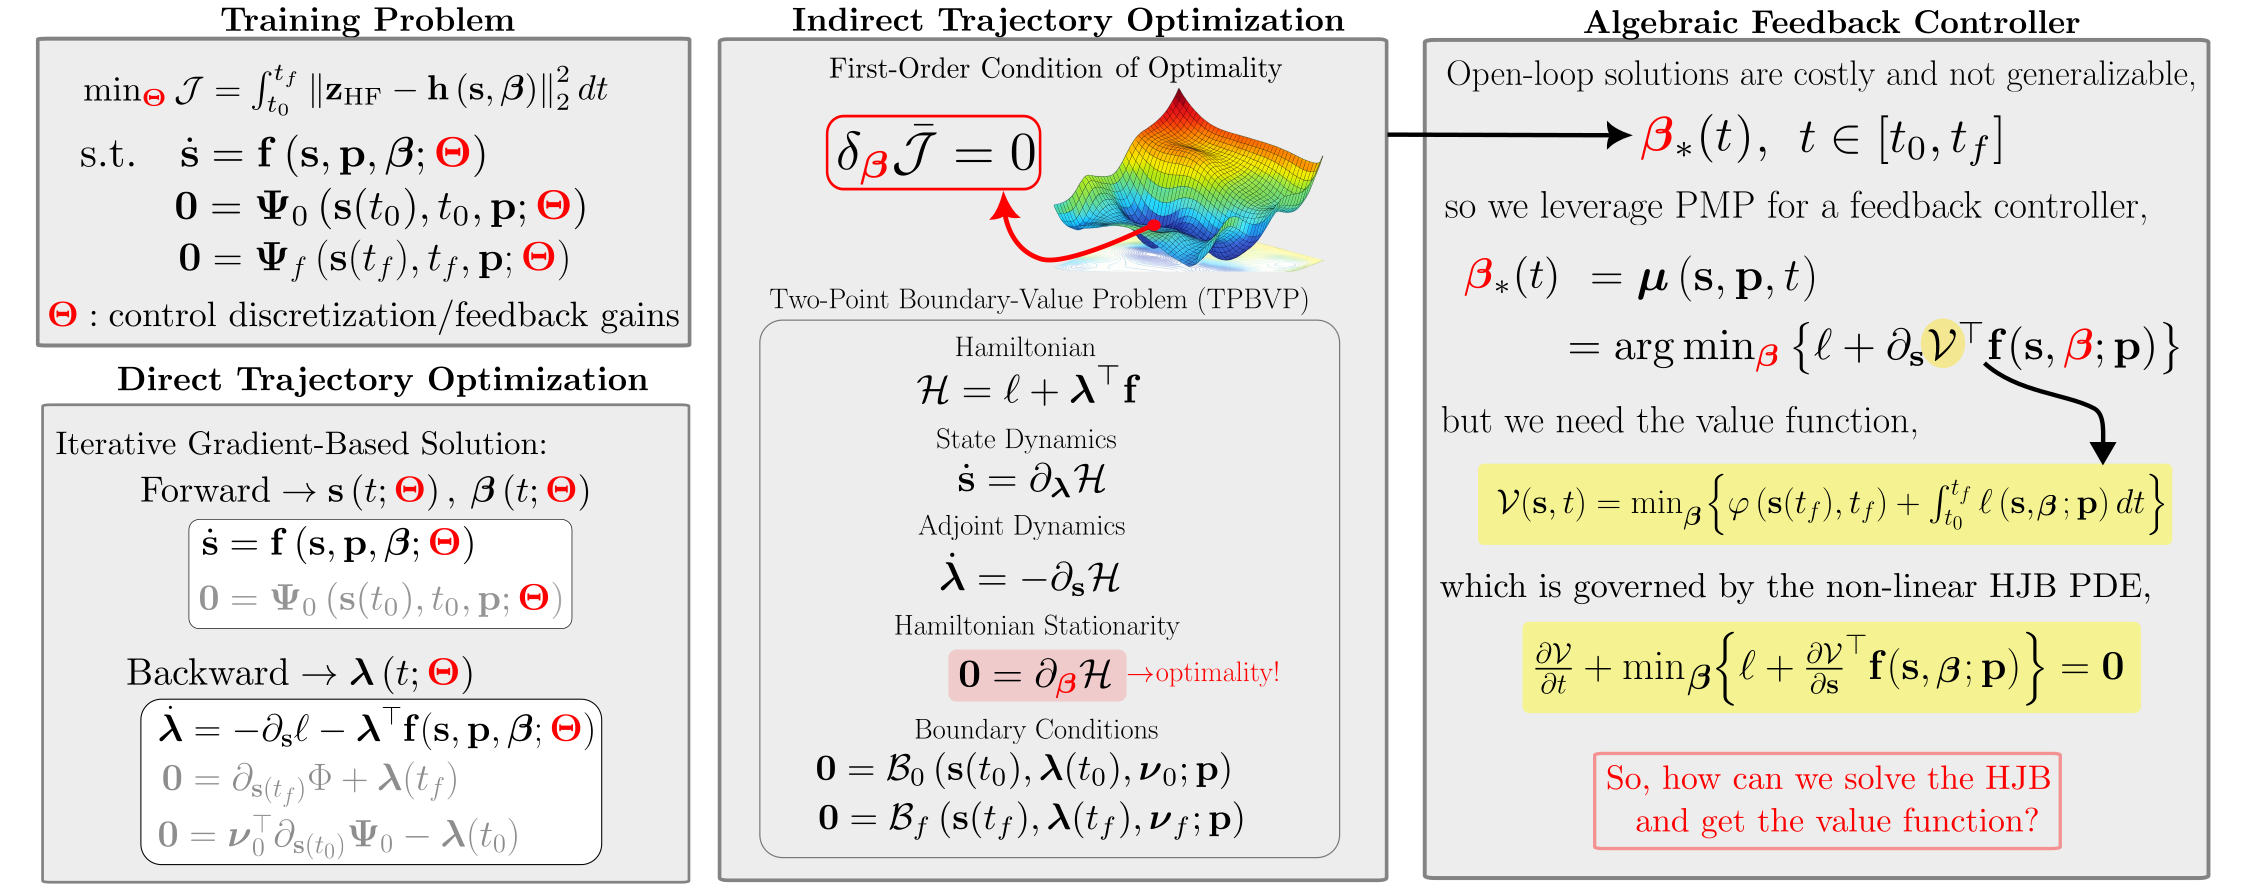
\includegraphics[width=0.95\textwidth]{../figs/ct/ct_overview_19.png}
        \end{figure}}
    \visible<2->{
    \begin{center}
        {\tiny
        $\vs$: state, $\Phi$: penalized terminal constraint, $\vbeta$: control action, $\cB_0,\cB_f$: boundary conditions, $\vnu$: Lagrange multipliers, $\vf$: non-linear dynamics, $\bar{\cJ}$: augmented cost functional, PMP: Pontryagin's Minimum Principle, HJB: Hamilton-Jacobi-Bellman
        }
    \end{center}}
\end{frame}

% \begin{frame}{\small Content Overview}
%     \footnotesize
%     \begin{enumerate}
%         \item \textcolor{gray!50}{Motivation, Background, and Objectives}
%         \item \textcolor{gray!50}{Addressing the Impossible Trinity of Modeling (ITM)}
%         \item \textcolor{gray!50}{Unified Control-Theoretic Training}
%         \item \colorbox{yellow!70}{\textbf{Addressing the Impossible Trinity of Optimal Control (ITOC)}}
%         \item \textcolor{gray!50}{Conclusions and Future Work}
%     \end{enumerate}
% \end{frame}

\begin{frame}
    \centering
    \Large\textbf{Addressing the Impossible Trinity of Optimal Control}
\end{frame}

\begin{frame}{\small How can we leverage the \textbf{control-theoretic} training for optimal closed-loop control?}
    \visible<2->{
    \begin{center}
        {\small \textbf{Consider the following example}:}\\
        {\small On-board optimal closed-loop control of a hypersonic vehicle}
    \end{center}
    \begin{figure}
        \centering
        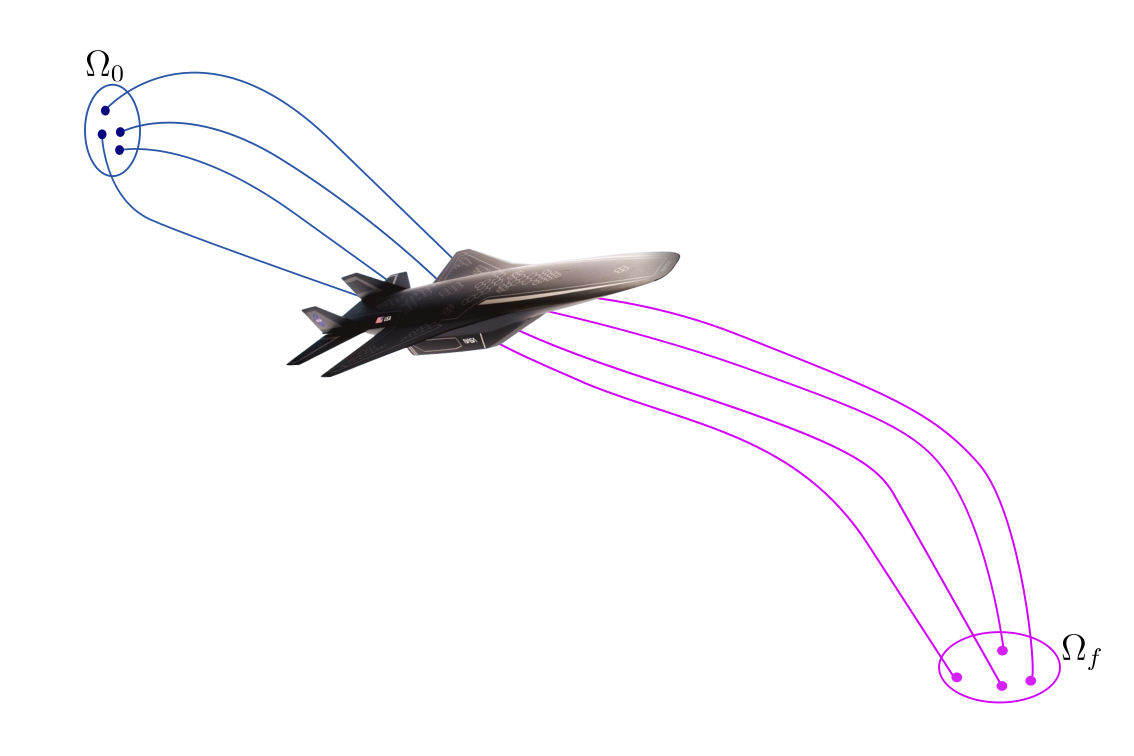
\includegraphics[width=0.6\textwidth]{../figs/introduction/motivating_example_1.png}
    \end{figure}}
\end{frame}

\begin{frame}{\small We want \textbf{accuracy, efficient, and generalizable} solutions to \textbf{non-linear OCPs},}
    \footnotesize
    \begin{columns}
        \begin{column}{0.7\textwidth}
            \only<2>{
                \begin{figure}
                    \centering
                    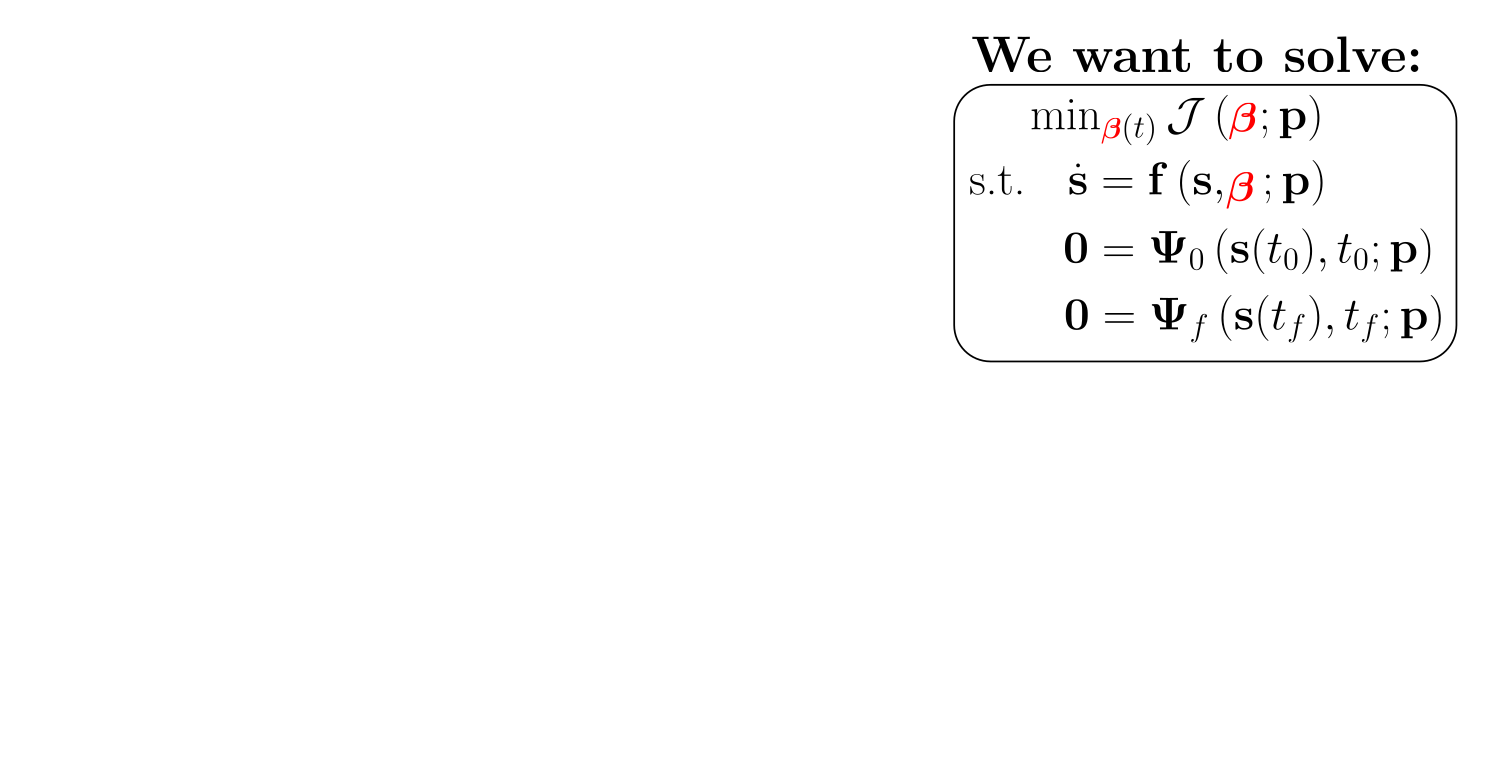
\includegraphics[width=0.9\textwidth]{../figs/sparsehjb/trajectory_parametrization_1.png}
                \end{figure}}
            \only<3>{
                \begin{figure}
                    \centering
                    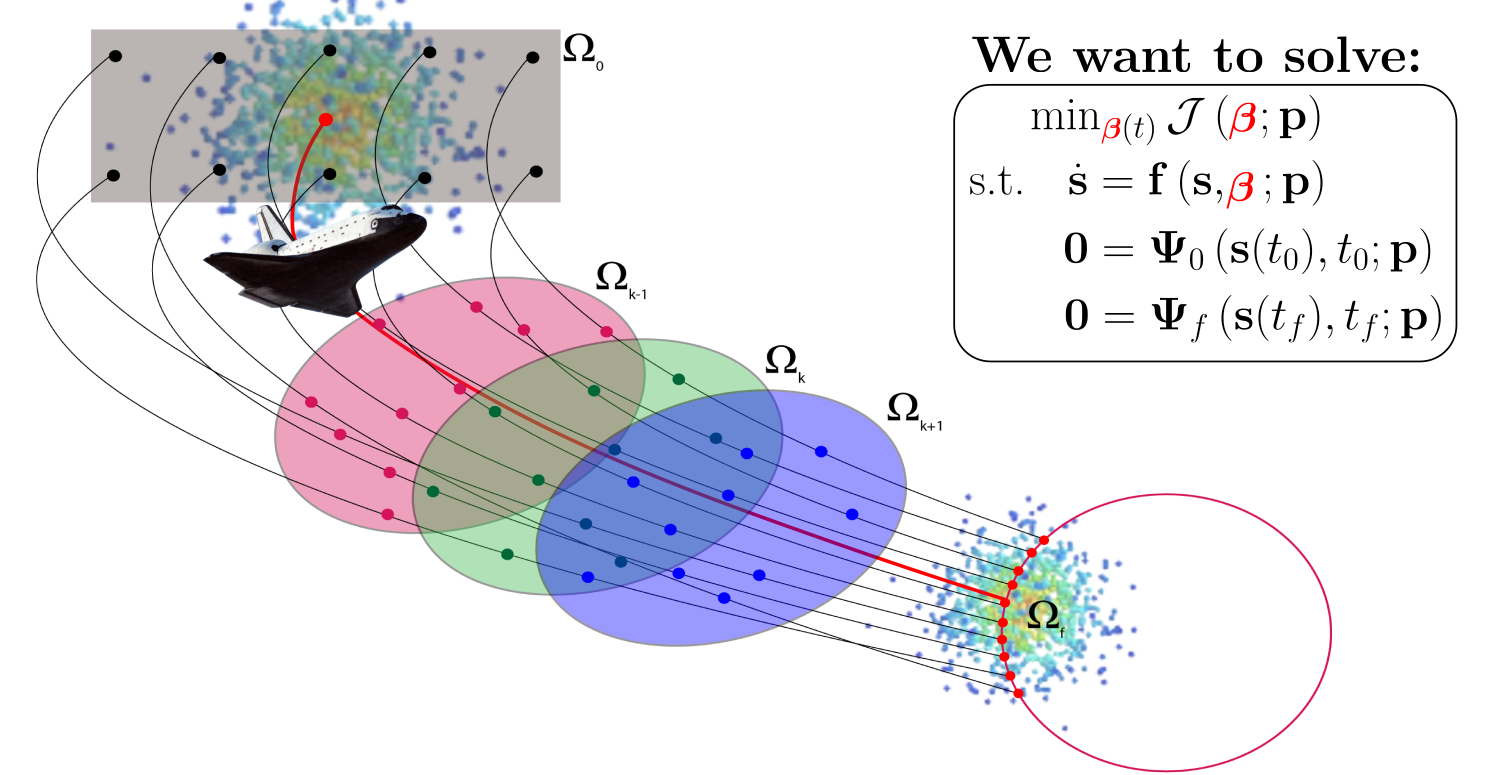
\includegraphics[width=0.9\textwidth]{../figs/sparsehjb/trajectory_parametrization_2.png}
                \end{figure}}
            \only<4->{
                \begin{figure}
                    \centering
                    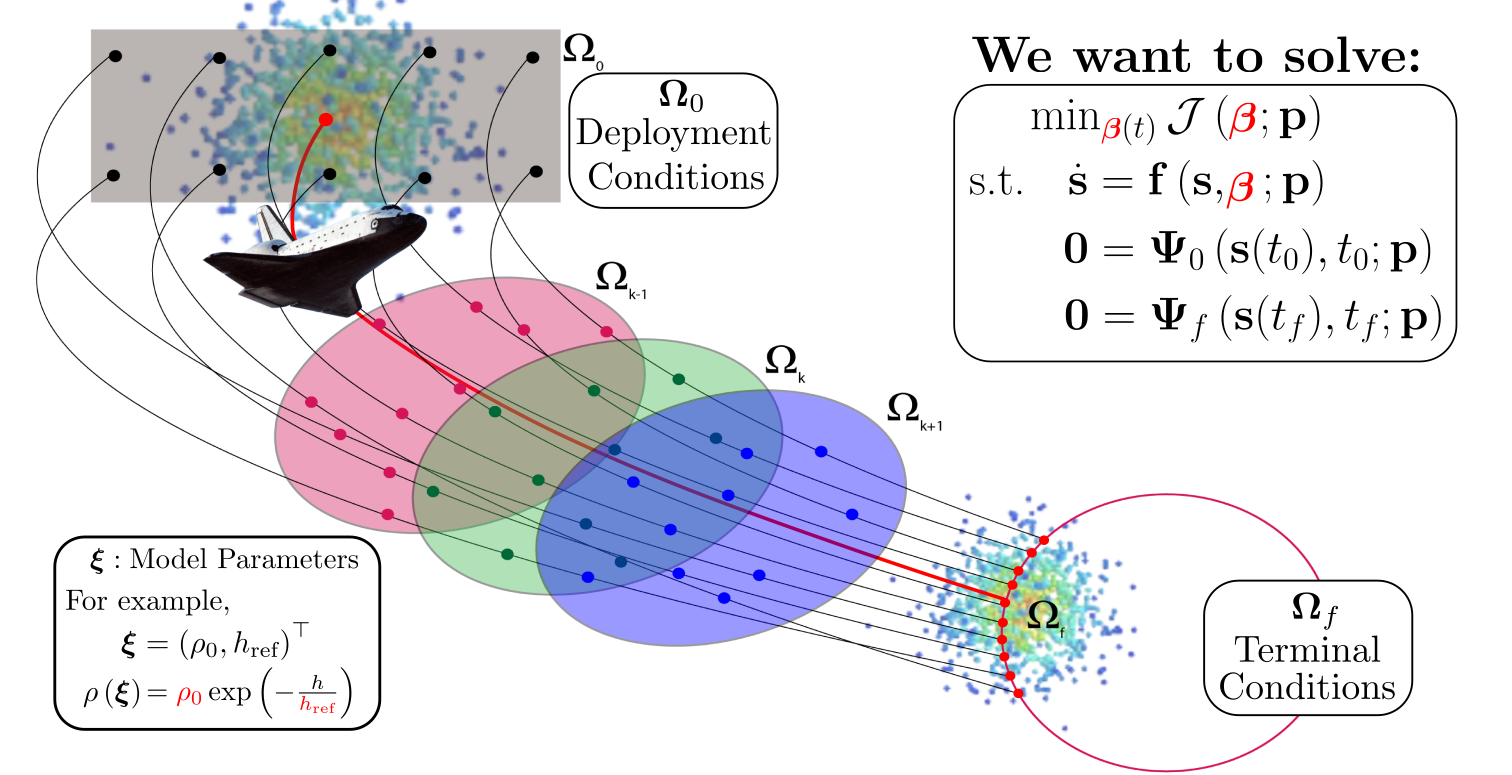
\includegraphics[width=0.9\textwidth]{../figs/sparsehjb/trajectory_parametrization_3.png}
                \end{figure}}
        \end{column}
        \hspace*{-0.5in}
        \begin{column}{0.4\textwidth}
            \visible<5->{
            \begin{graybox}{Parametrization}
                \visible<6->{
                Parameters,
                \begin{equation*}
                    \vp = \left(\vOmega_0,\vOmega_f,\vxi\right)^\top\in\mathbb{R}^{n_p}
                \end{equation*}}
                \visible<7->{
                are, e.g., normally distributed,
                \begin{equation*}
                    \vp\sim\mathcal{N}\left(\mathbf{m},\boldsymbol{\sigma}\right)
                \end{equation*}}
                \visible<8->{
                where,
                \begin{itemize}
                    \item $\mathbf{m}$: nominal mission,
                    \item $\boldsymbol{\sigma}$: mission uncertainty
                \end{itemize}}
            \end{graybox}}
        \end{column}
    \end{columns}
\end{frame}

\begin{frame}{\small Generate a sparse high fidelity \textbf{distribution of optimal paths},}
    \footnotesize
    \only<1>{
        \begin{figure}
            \centering
            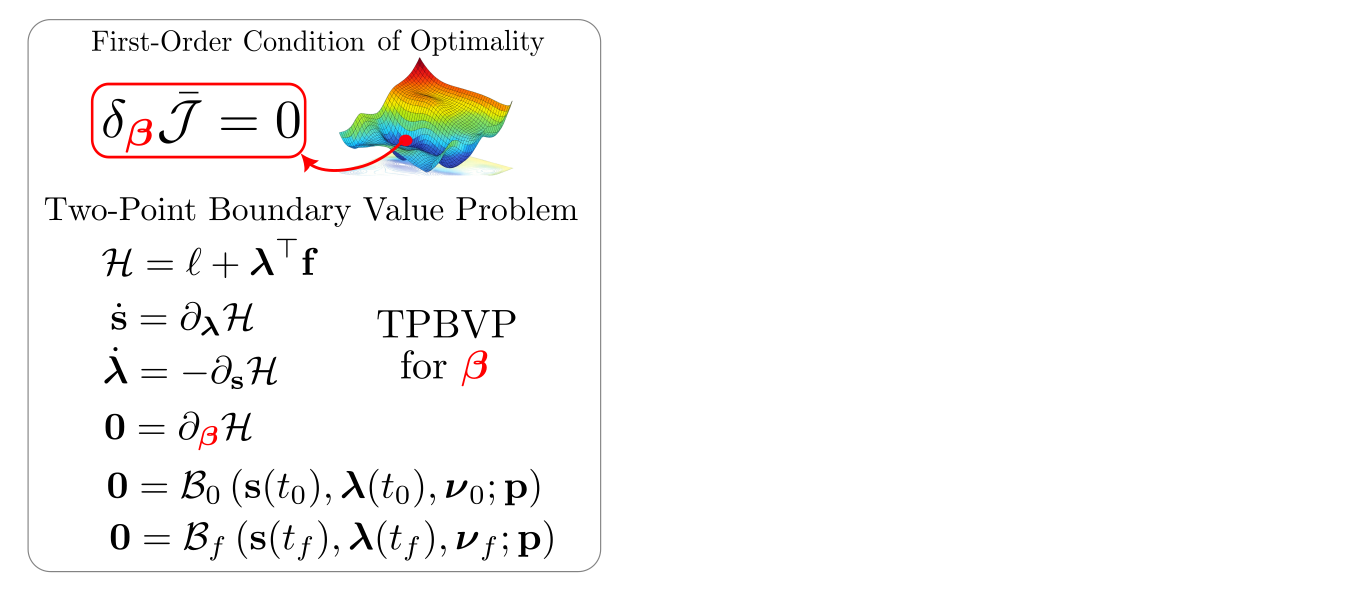
\includegraphics[width=0.9\textwidth]{../figs/sparsehjb/solutions_1.png}
        \end{figure}}
    \only<2>{
        \begin{figure}
            \centering
            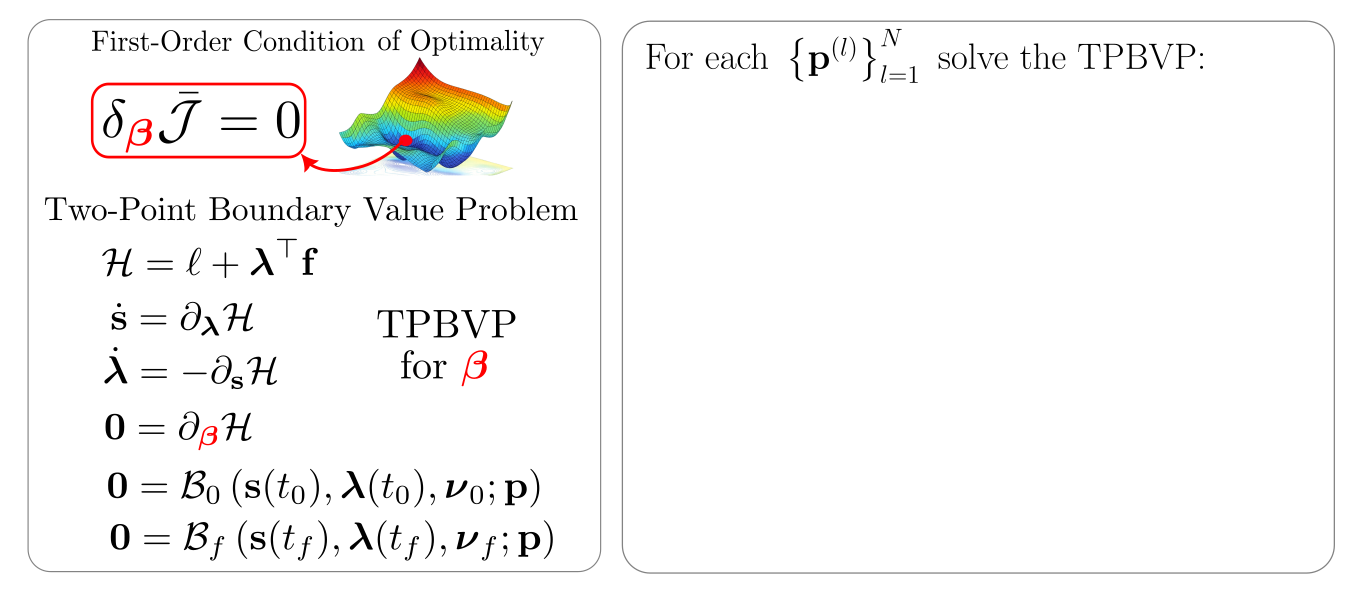
\includegraphics[width=0.9\textwidth]{../figs/sparsehjb/solutions_2.png}
        \end{figure}}
    \only<3>{
        \begin{figure}
            \centering
            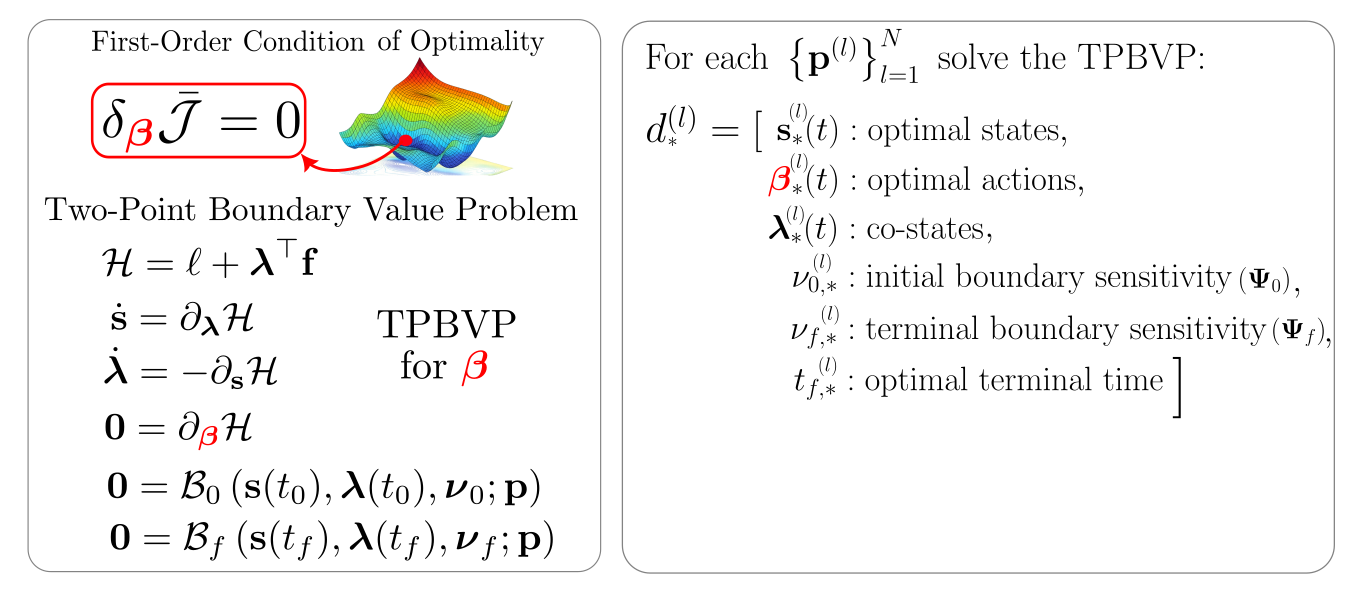
\includegraphics[width=0.9\textwidth]{../figs/sparsehjb/solutions_3.png}
        \end{figure}}
    \only<4>{
        \begin{figure}
            \centering
            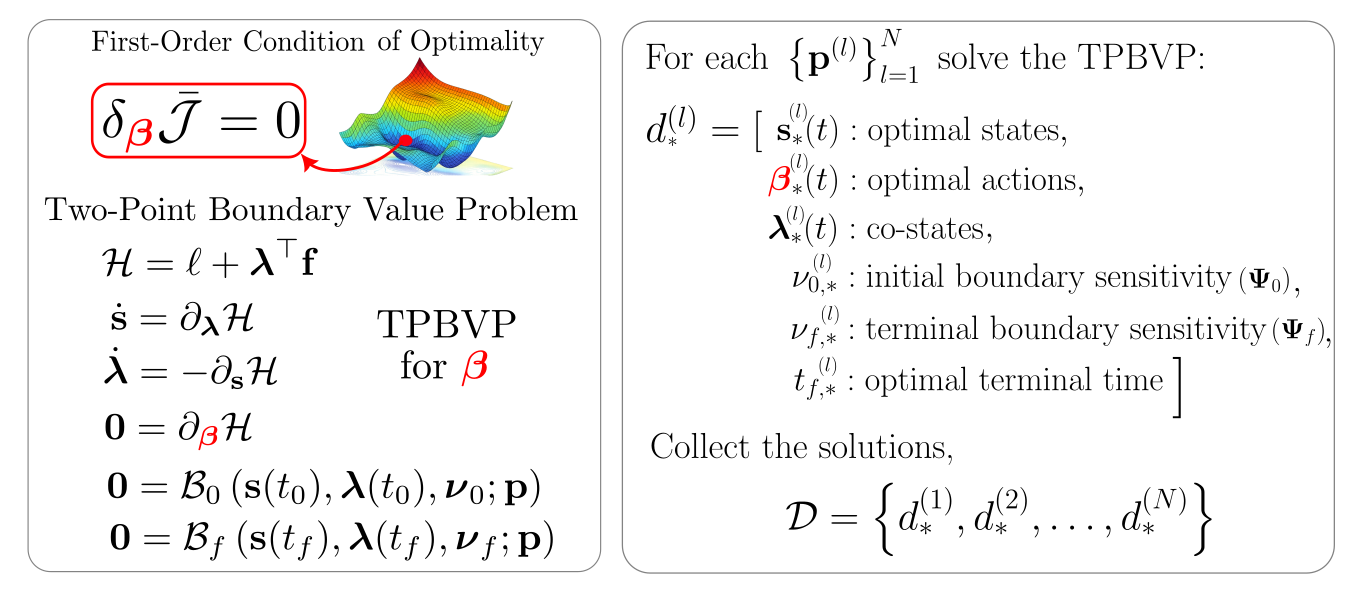
\includegraphics[width=0.9\textwidth]{../figs/sparsehjb/solutions_4.png}
        \end{figure}}
\end{frame}

\begin{frame}{\small \textbf{Learn the value function} from the sparse high fidelity data,}
    \footnotesize
    \only<2>{
        \begin{figure}
            \centering
            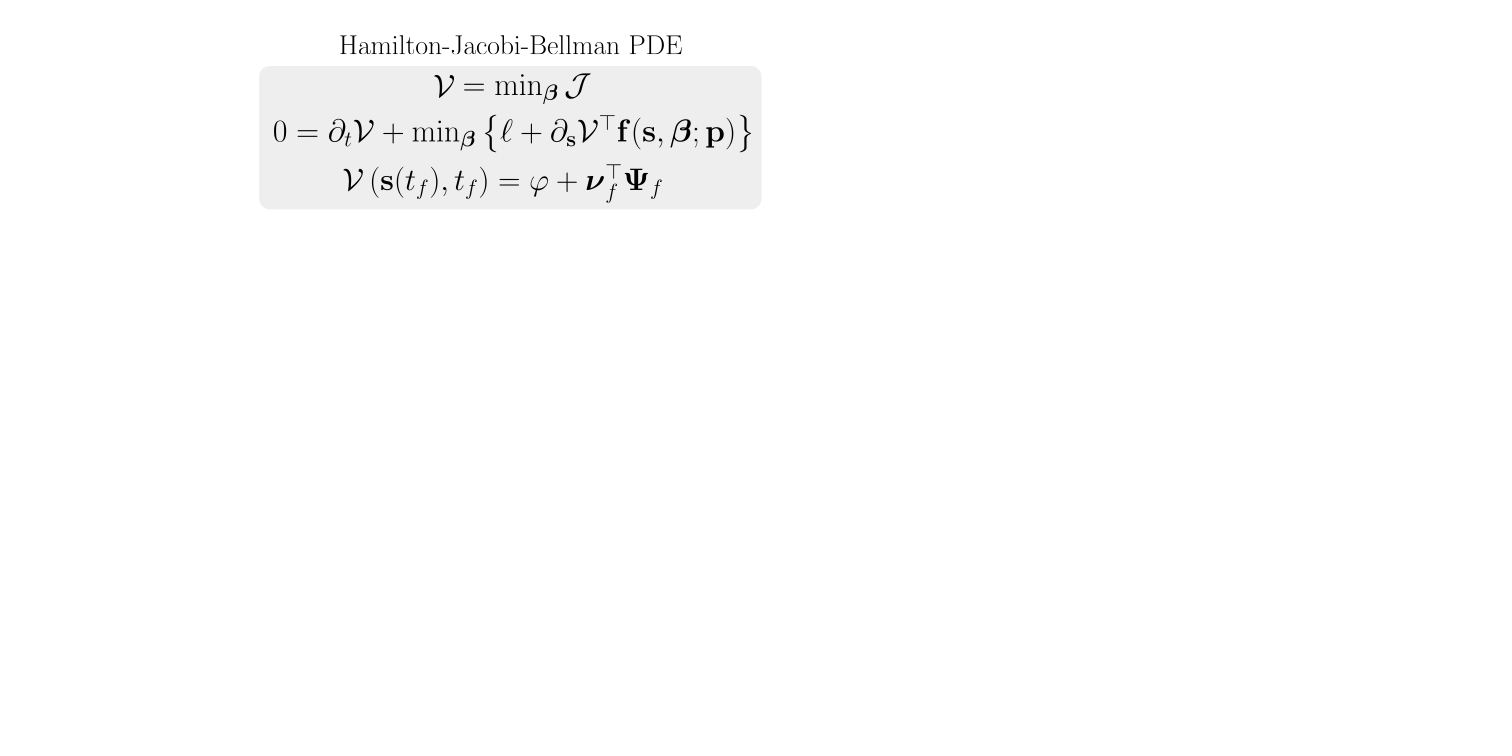
\includegraphics[width=0.95\textwidth]{../figs/sparsehjb/characteristics_1.png}
        \end{figure}}
    \only<3>{
        \begin{figure}
            \centering
            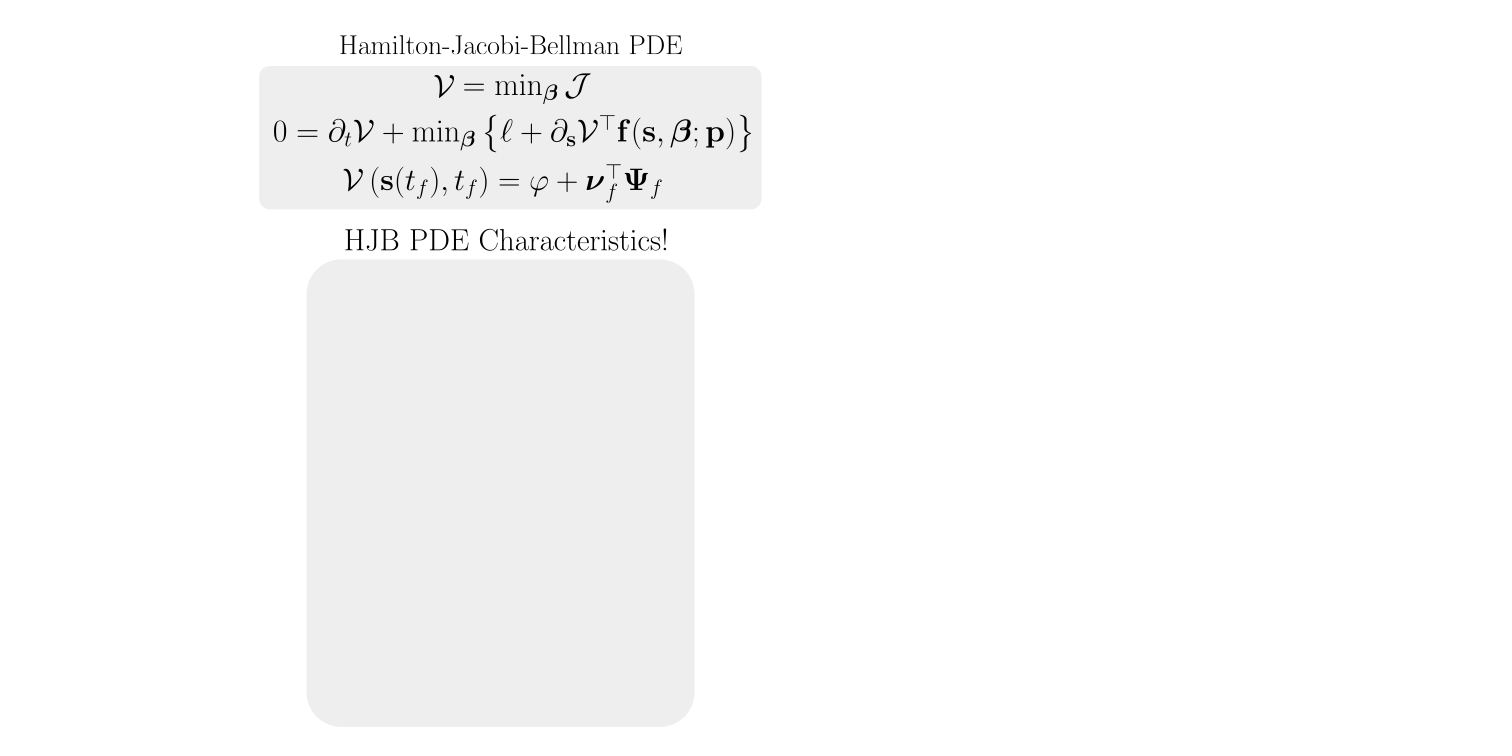
\includegraphics[width=0.95\textwidth]{../figs/sparsehjb/characteristics_2.png}
        \end{figure}}
    \only<4>{
        \begin{figure}
            \centering
            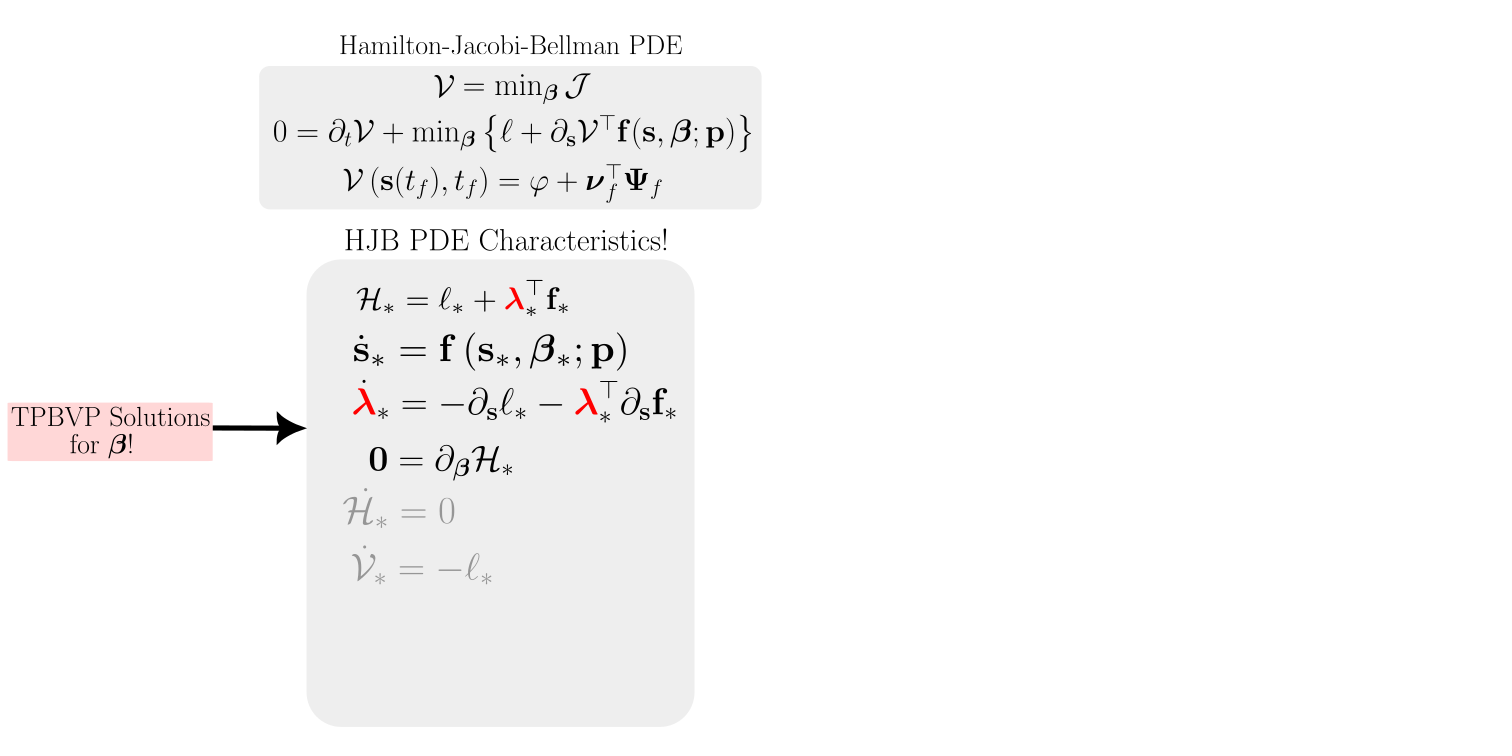
\includegraphics[width=0.95\textwidth]{../figs/sparsehjb/characteristics_3.png}
        \end{figure}}
    \only<5>{
        \begin{figure}
            \centering
            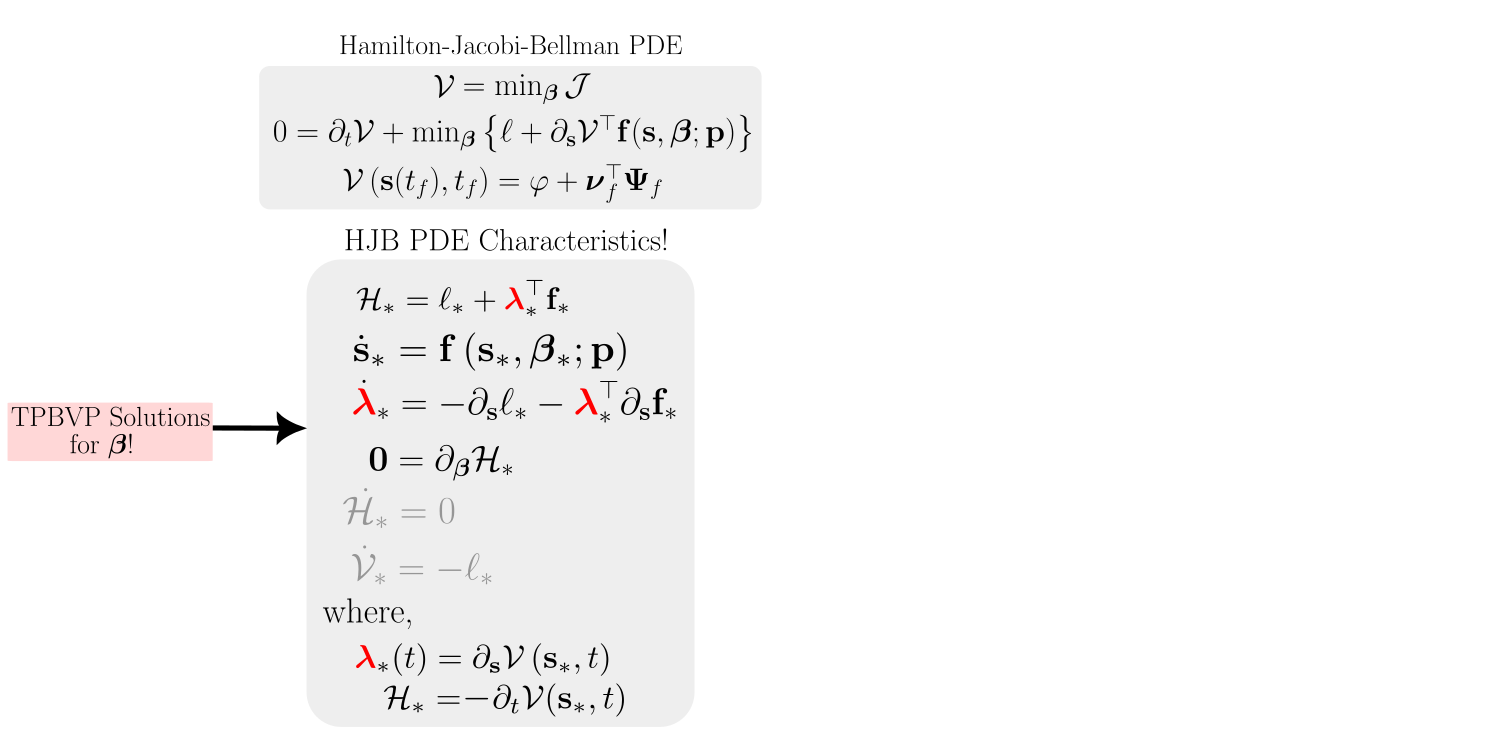
\includegraphics[width=0.95\textwidth]{../figs/sparsehjb/characteristics_4.png}
        \end{figure}}
    \only<6>{
        \begin{figure}
            \centering
            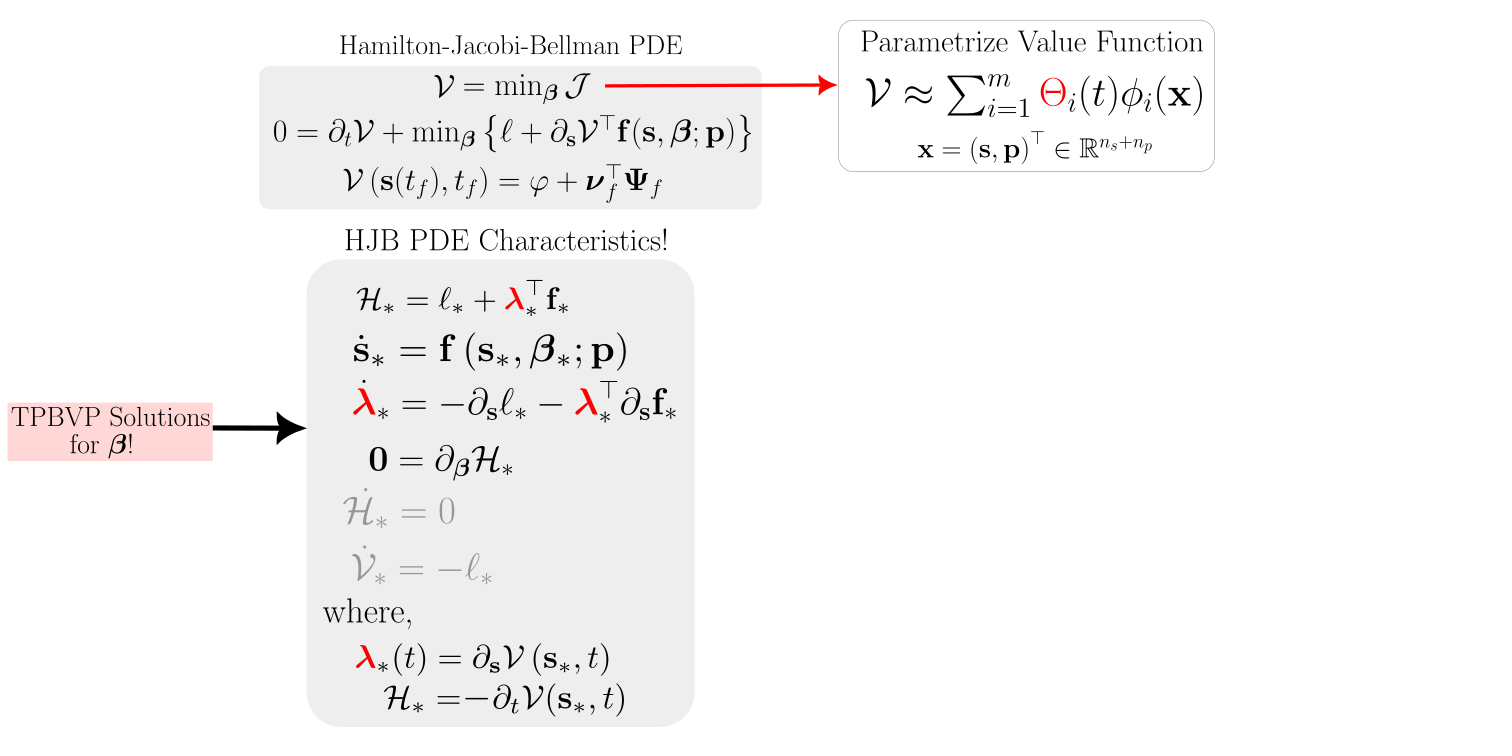
\includegraphics[width=0.95\textwidth]{../figs/sparsehjb/characteristics_5.png}
        \end{figure}}
    \only<7>{
        \begin{figure}
            \centering
            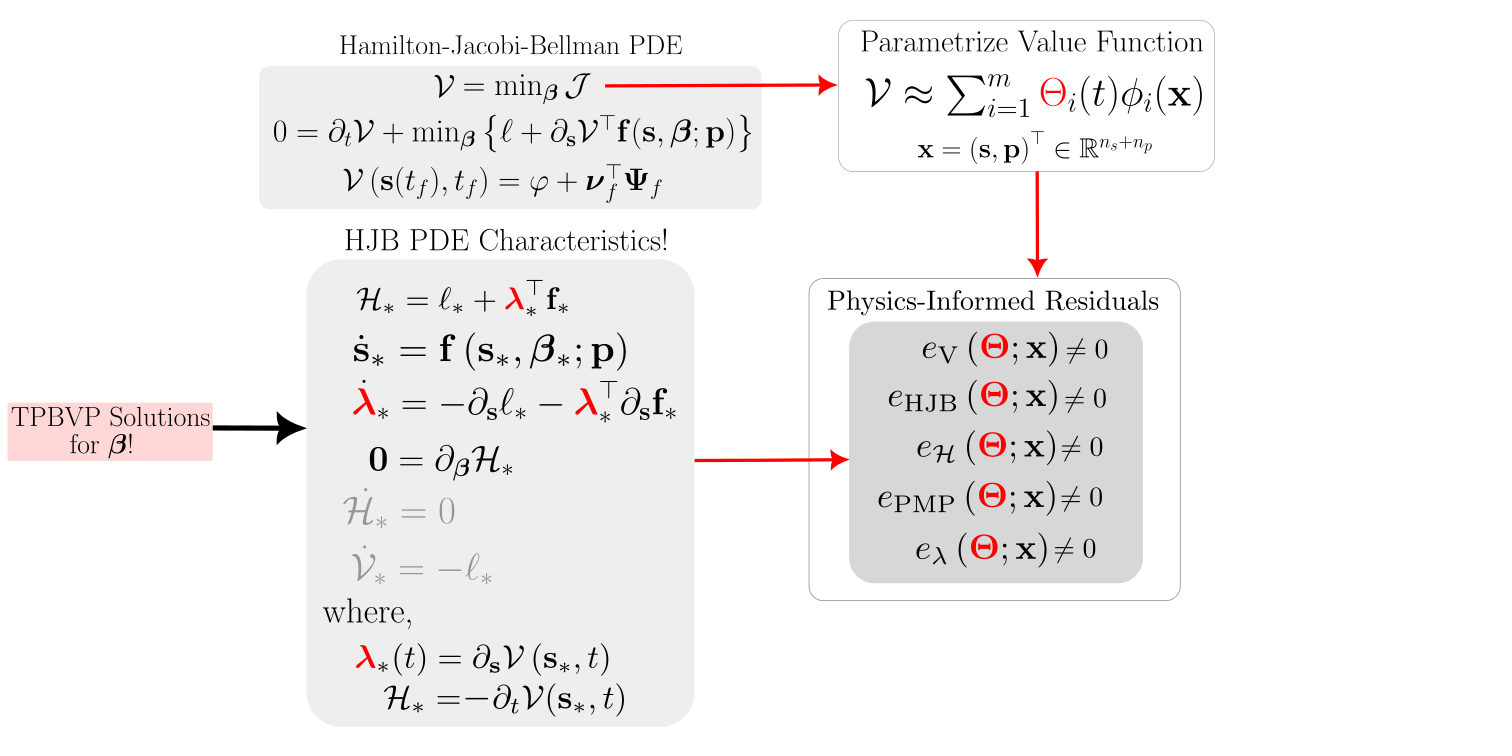
\includegraphics[width=0.95\textwidth]{../figs/sparsehjb/characteristics_6.png}
        \end{figure}}
    \only<8>{
        \begin{figure}
            \centering
            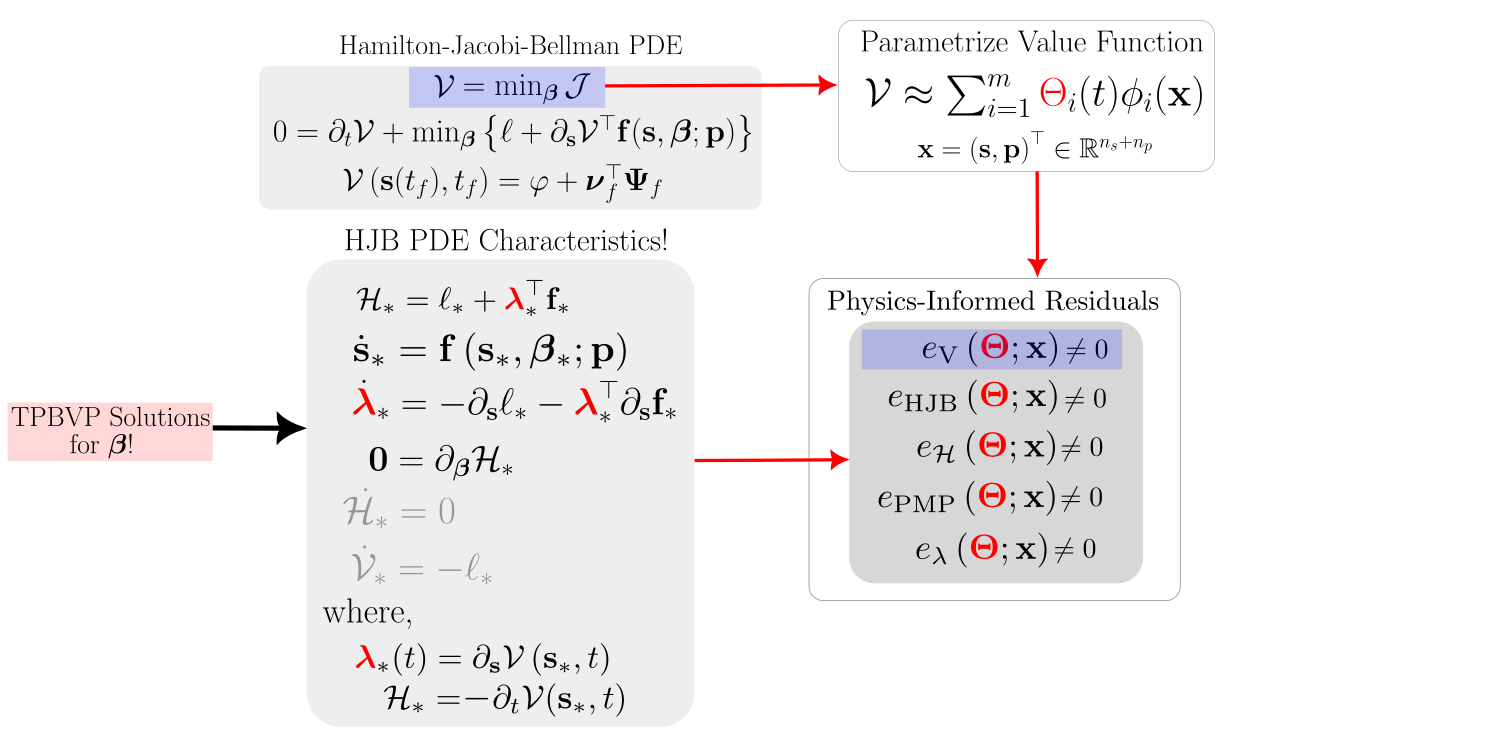
\includegraphics[width=0.95\textwidth]{../figs/sparsehjb/characteristics_7.png}
        \end{figure}}
    \only<9>{
        \begin{figure}
            \centering
            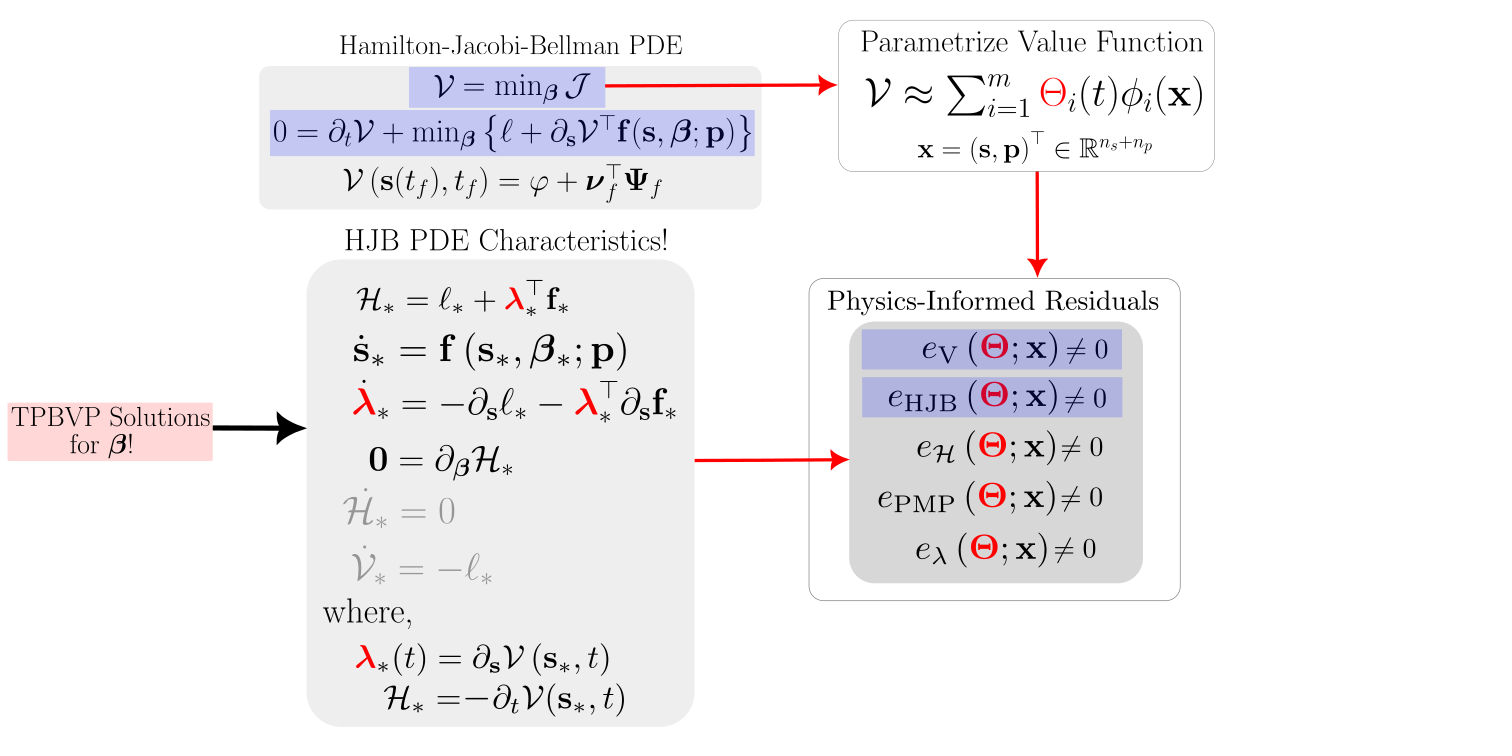
\includegraphics[width=0.95\textwidth]{../figs/sparsehjb/characteristics_8.png}
        \end{figure}}
    \only<10>{
        \begin{figure}
            \centering
            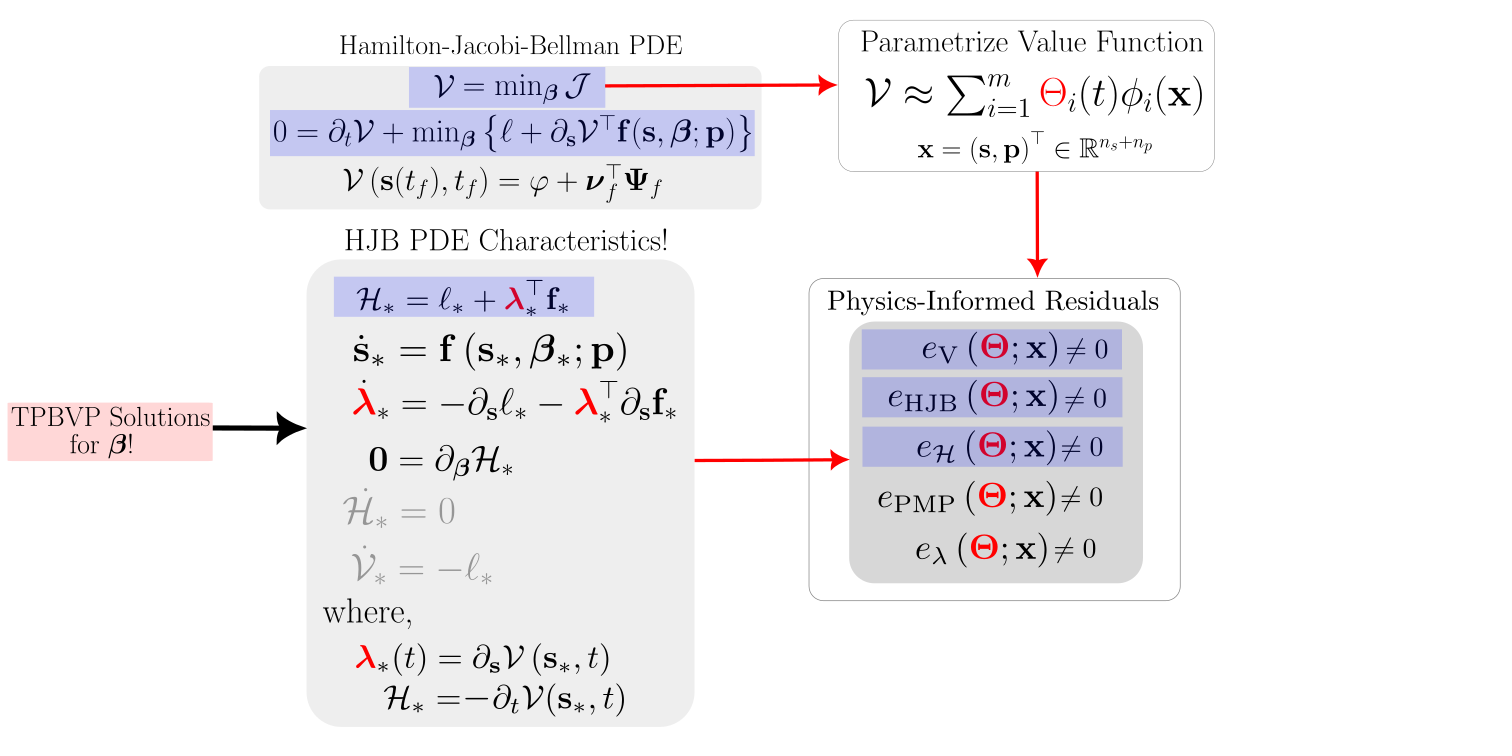
\includegraphics[width=0.95\textwidth]{../figs/sparsehjb/characteristics_9.png}
        \end{figure}}
    \only<11>{
        \begin{figure}
            \centering
            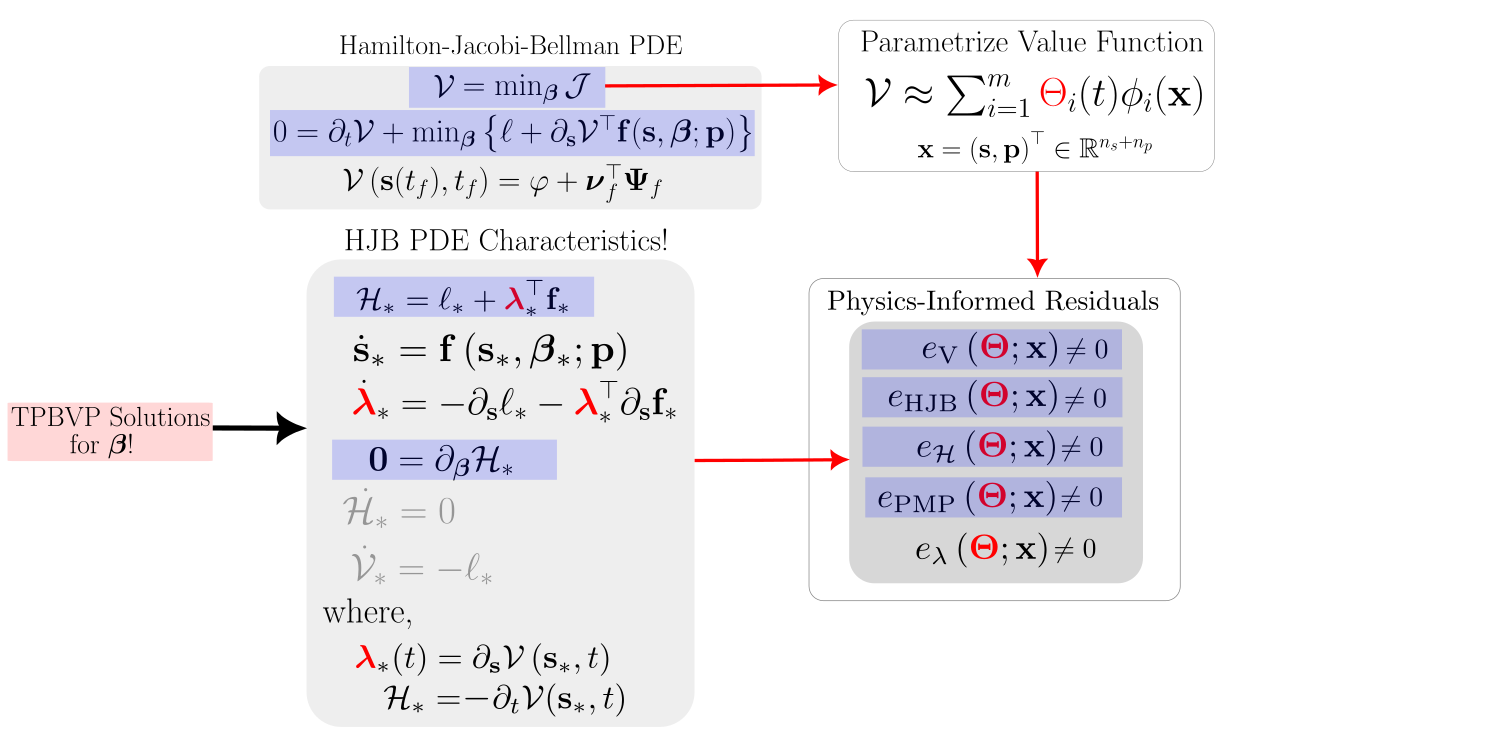
\includegraphics[width=0.95\textwidth]{../figs/sparsehjb/characteristics_10.png}
        \end{figure}}
    \only<12>{
        \begin{figure}
            \centering
            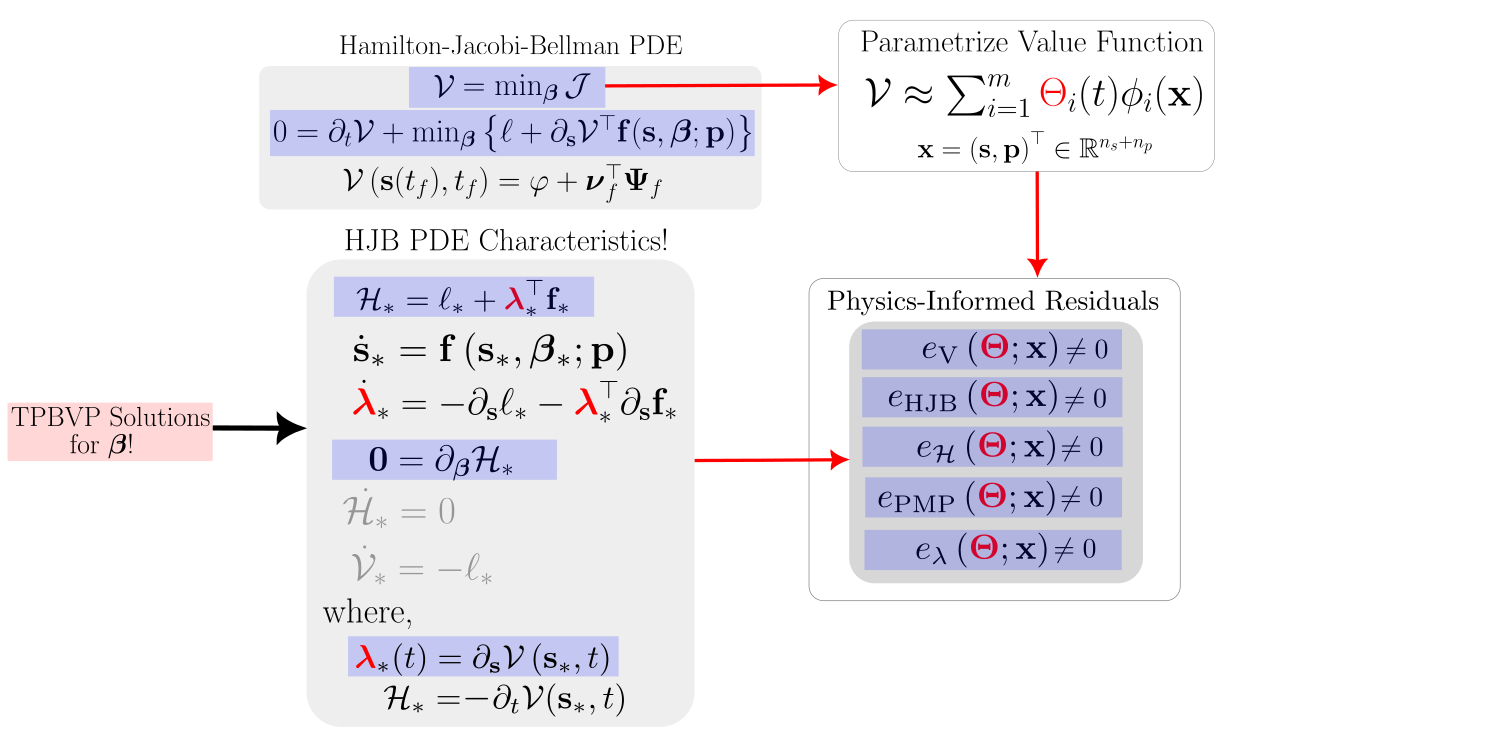
\includegraphics[width=0.95\textwidth]{../figs/sparsehjb/characteristics_11.png}
        \end{figure}}
    \only<13>{
        \begin{figure}
            \centering
            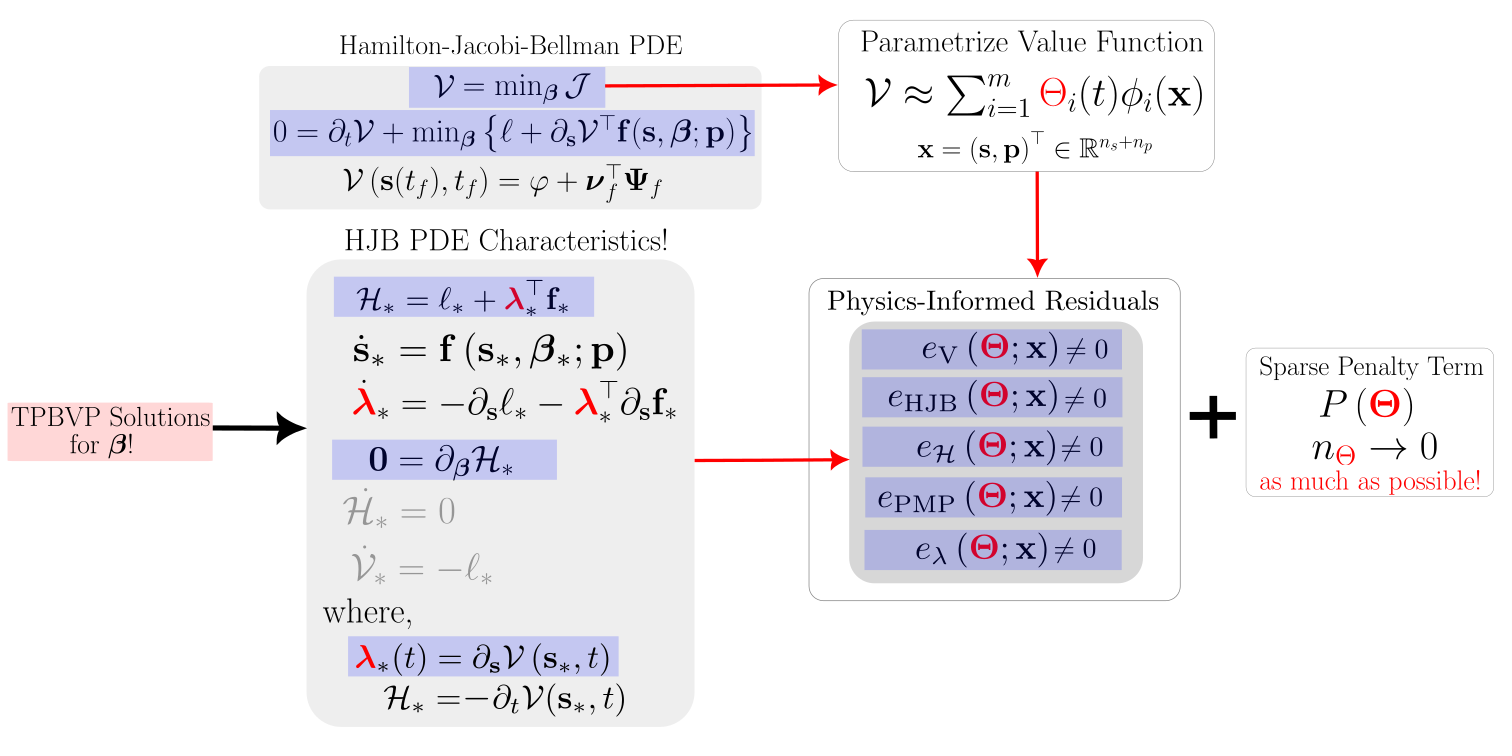
\includegraphics[width=0.95\textwidth]{../figs/sparsehjb/characteristics_12.png}
        \end{figure}}
\end{frame}

\begin{frame}{\small We can \textbf{learn the value function} with controllable \textbf{efficiency and accuracy},}
    \footnotesize
    \only<2>{
        \begin{figure}
            \centering
            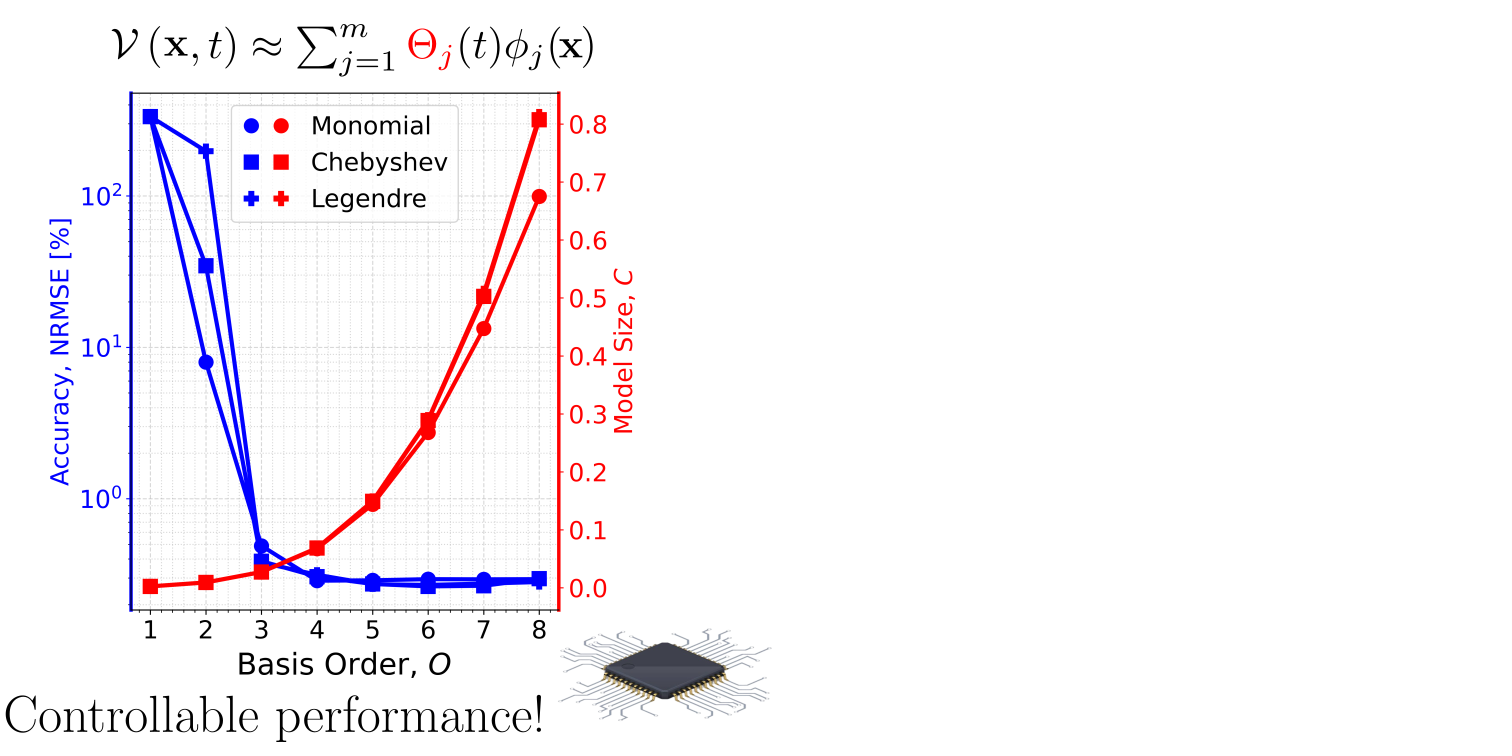
\includegraphics[width=0.9\textwidth]{../figs/sparsehjb/performance_ae_1.png}
        \end{figure}}
    \only<3>{
        \begin{figure}
            \centering
            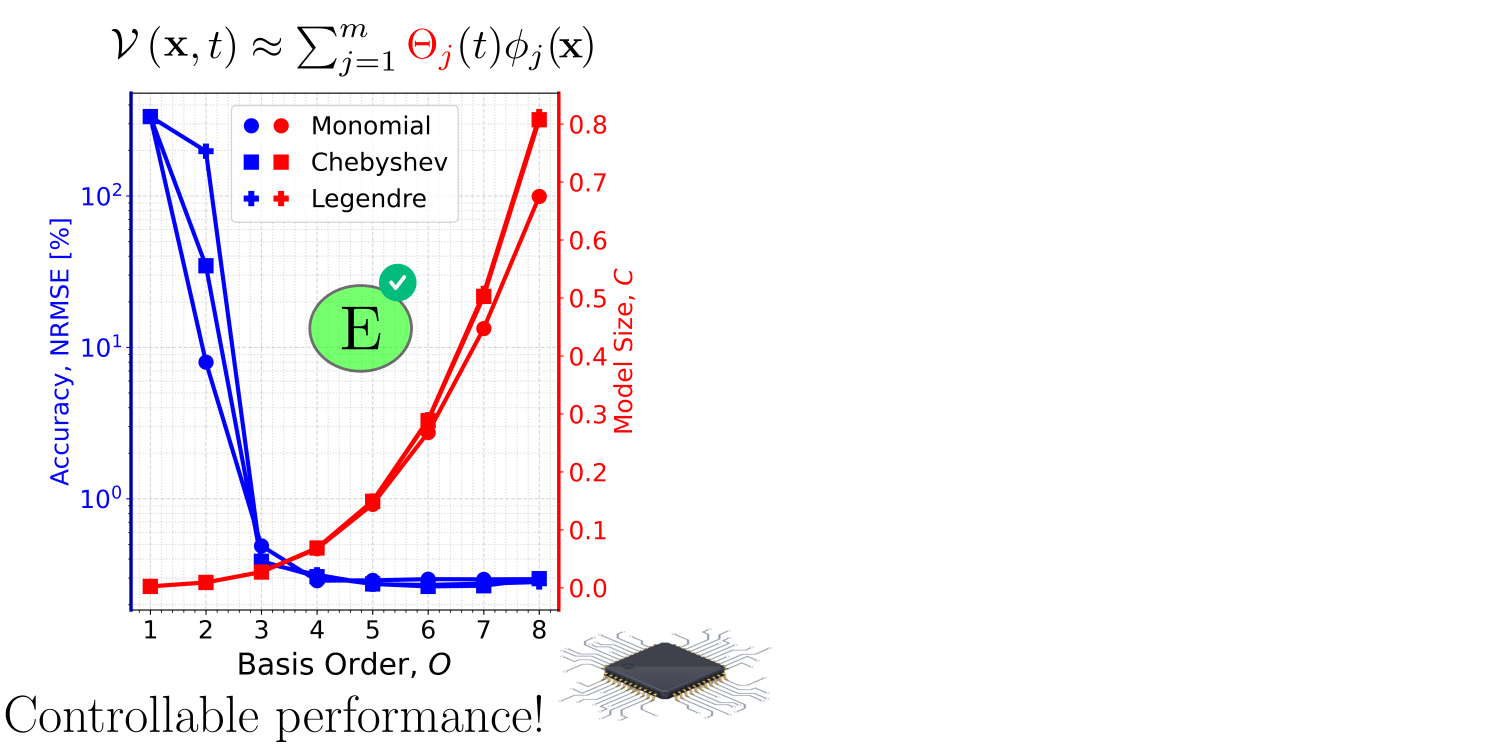
\includegraphics[width=0.9\textwidth]{../figs/sparsehjb/performance_ae_2.png}
        \end{figure}}
    \only<4>{
        \begin{figure}
            \centering
            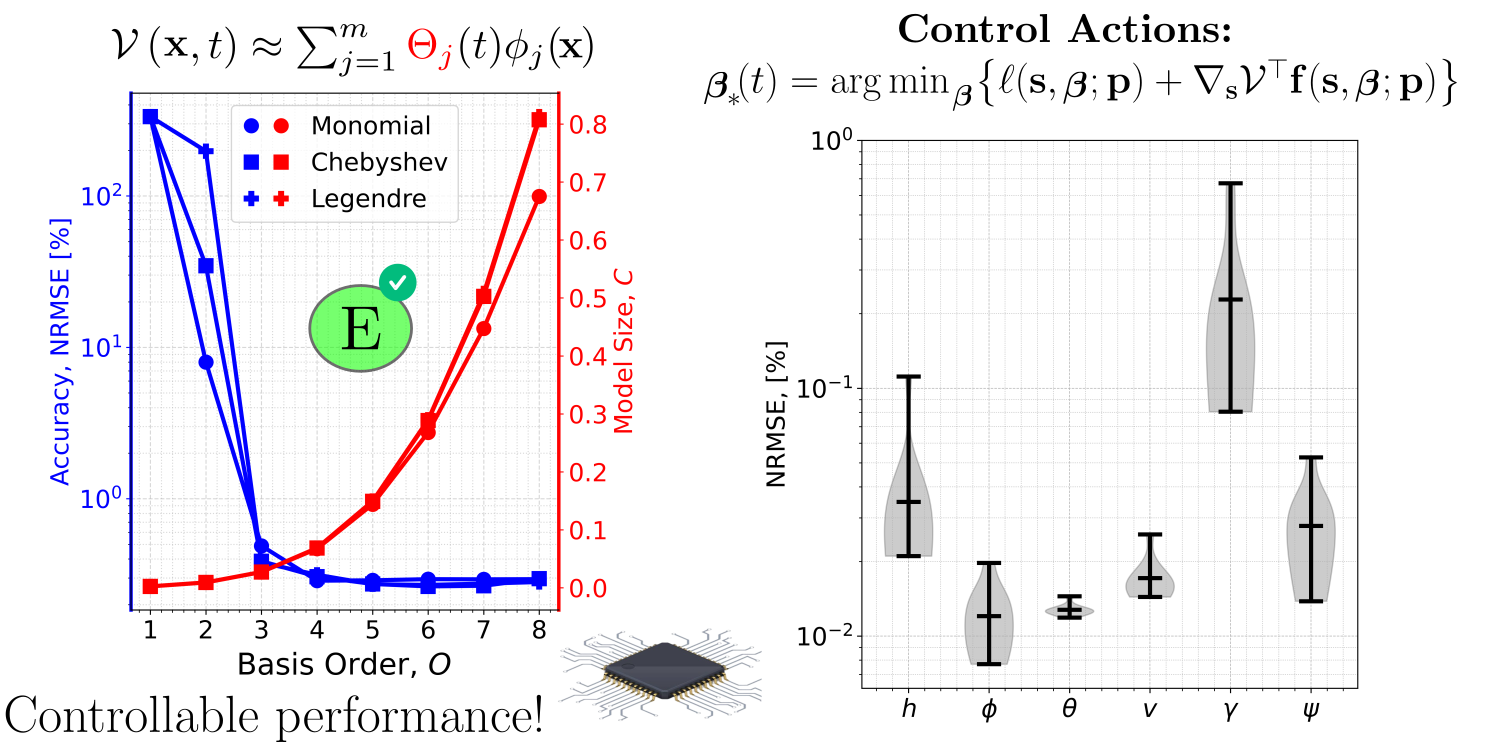
\includegraphics[width=0.9\textwidth]{../figs/sparsehjb/performance_ae_3.png}
        \end{figure}}
    \only<5>{
        \begin{figure}
            \centering
            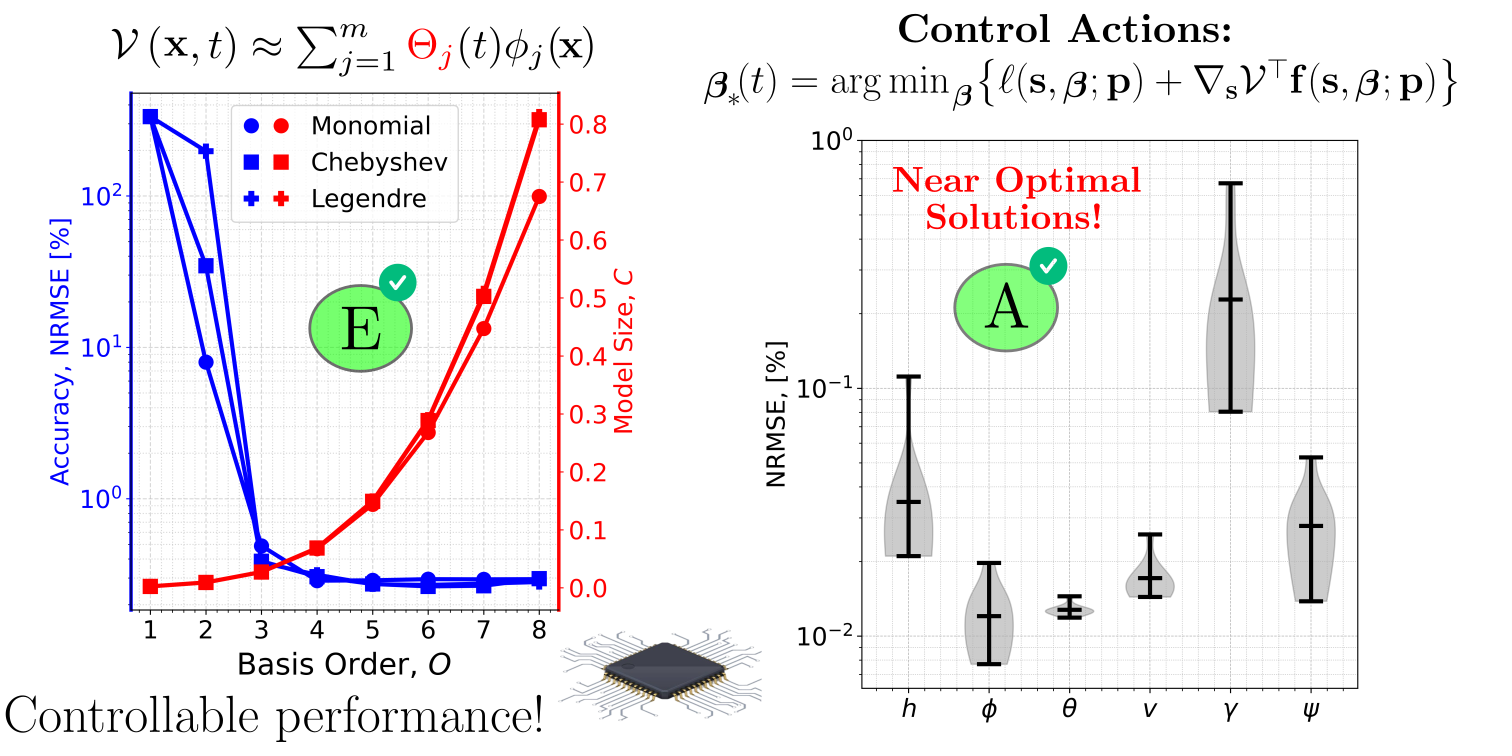
\includegraphics[width=0.9\textwidth]{../figs/sparsehjb/performance_ae_4.png}
        \end{figure}}
\end{frame}

\begin{frame}{\small Real-time control for the \textbf{space shuttle during re-entry} to maximize \textbf{cross-range},}
    \footnotesize
    \begin{columns}
        \begin{column}{0.7\textwidth}
            \only<2>{
                \begin{figure}
                    \centering
                    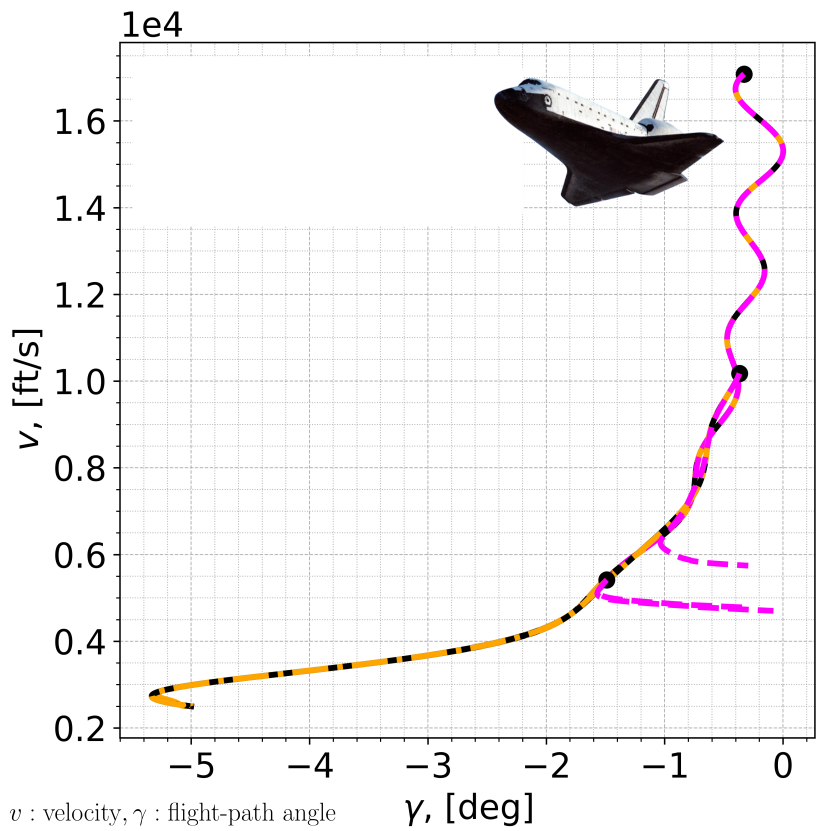
\includegraphics[width=0.65\textwidth]{../figs/sparsehjb/performance_ss_1.png}
                \end{figure}}
            \only<3>{
                \begin{figure}
                    \centering
                    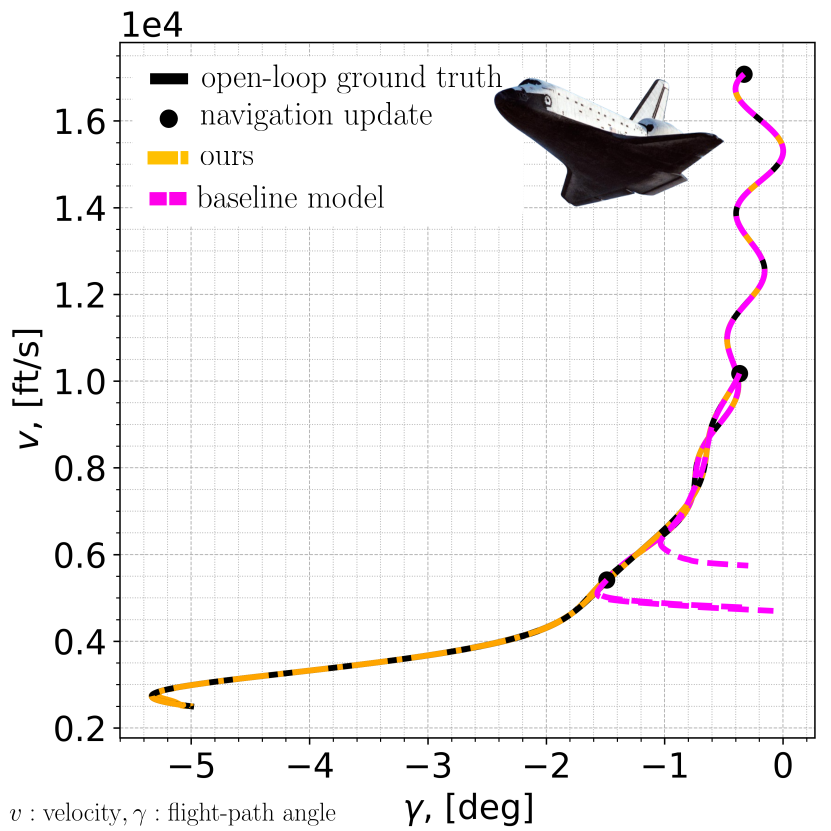
\includegraphics[width=0.65\textwidth]{../figs/sparsehjb/performance_ss_2.png}
                \end{figure}}
            \only<4>{
                \begin{figure}
                    \centering
                    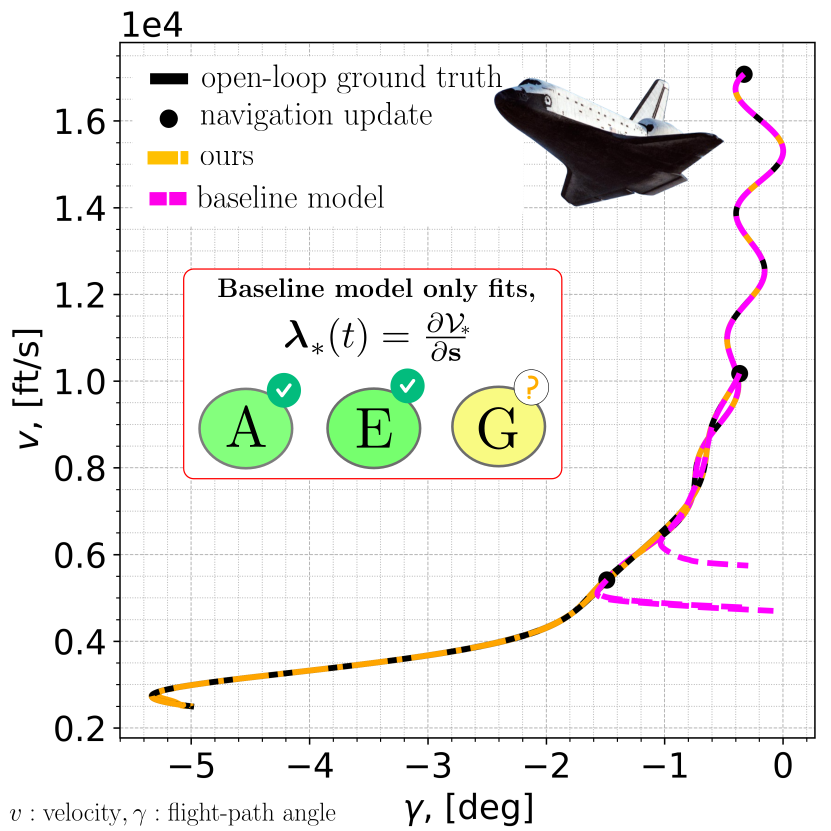
\includegraphics[width=0.65\textwidth]{../figs/sparsehjb/performance_ss_3.png}
                \end{figure}}
            \only<5->{
                \begin{figure}
                    \centering
                    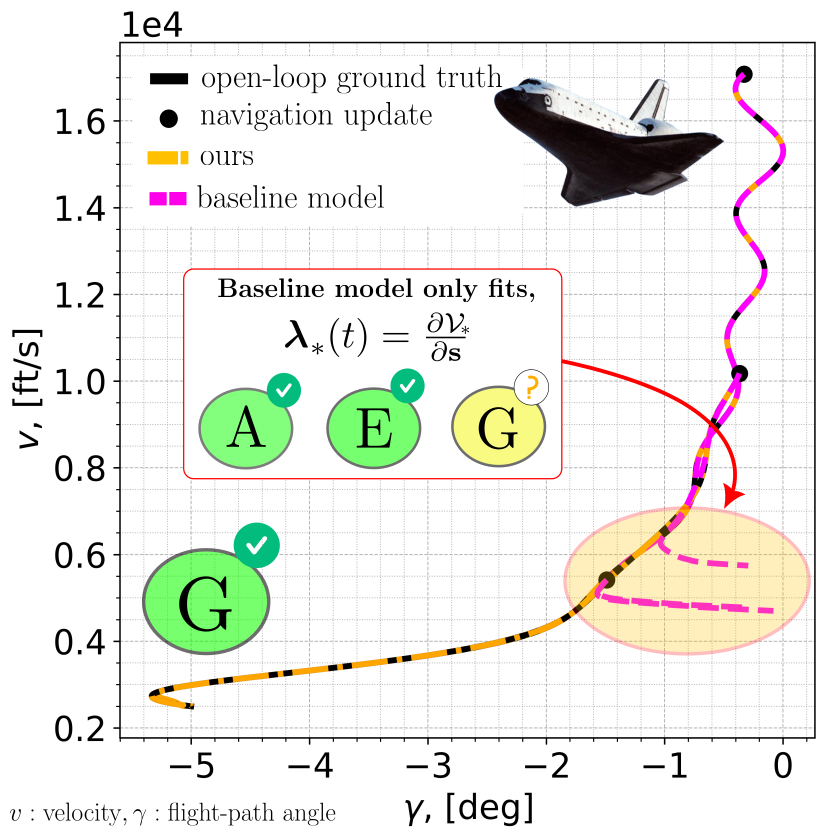
\includegraphics[width=0.65\textwidth]{../figs/sparsehjb/performance_ss_4.png}
                \end{figure}}
        \end{column}
        \hspace*{-1in}
        \begin{column}{0.4\textwidth}
            \visible<6->{
            \begin{graybox}{Key Results}
                \begin{itemize}
                    \item Improved \textbf{generalizability},
                    \item \textbf{Accelerations} $\approx10^4$,
                    \item \textbf{Model compressions} $\approx30\%$
                \end{itemize}
            \end{graybox}}
        \end{column}
    \end{columns}
\end{frame}

\begin{frame}{\small Is the Impossible Trinity of Optimal Control \textbf{solved}?}
    \footnotesize
    \begin{columns}
        \begin{column}{0.4\textwidth}
            \centering
            \visible<2->{
            \begin{figure}
                \centering
                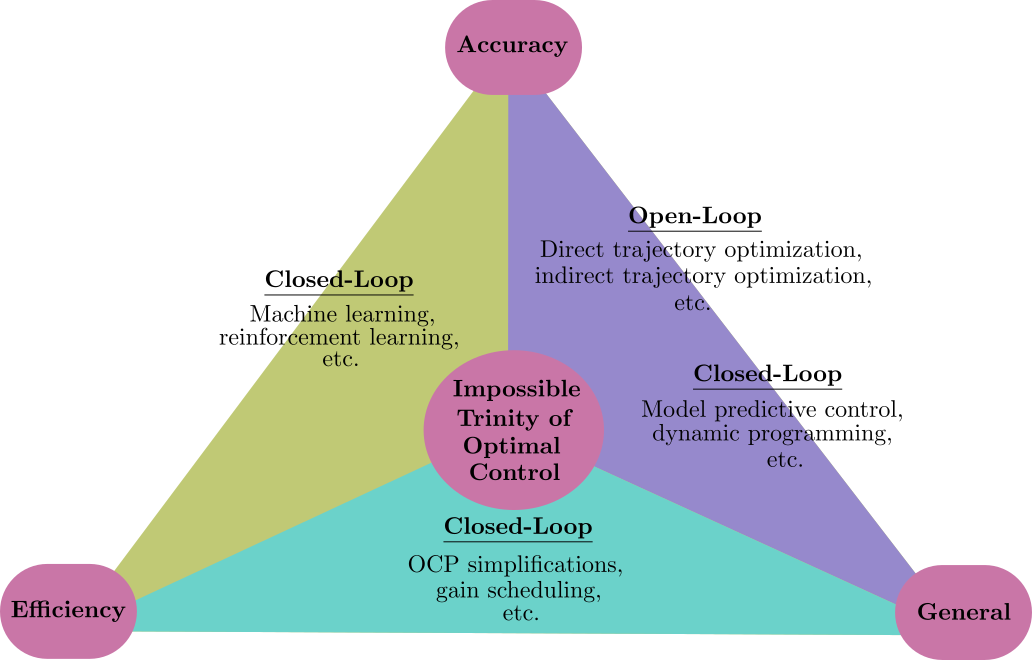
\includegraphics[width=0.9\textwidth]{../figs/introduction/itoc.png}
            \end{figure}}
        \end{column}
        \begin{column}{0.7\textwidth}
            \centering
            \begin{itemize}
                \item<3-> \textbf{Accuracy}: comparable to indirect OCP solutions (NRMSE $<1\%$)
                \item<4-> \colorbox{green!30}{\textbf{Efficiency}}:
                \begin{itemize}
                    \item<5-> \colorbox{green!30}{\textbf{Accelerations} $\approx 10^3 - 10^4$}
                    \item<6-> \colorbox{green!30}{\textbf{Model compressions} $\approx 80\%$}
                \end{itemize}
                \item<7-> \colorbox{green!30}{\textbf{Generalizability}: unseen BCs and model parameters}, but no guarantees outside the tube!
                \item<8-> Offline training costs \colorbox{red!30}{not quantified (future work)}
            \end{itemize}
        \end{column}
    \end{columns}
    \visible<3->{
    \begin{tikzpicture}[remember picture, overlay]
        \node[anchor=north west, xshift=2.2cm, yshift=-2.2cm] at (current page.north west) {
\includegraphics[width=0.1\textwidth]{../figs/pirom/checkmark.png}};
    \end{tikzpicture}}
    \visible<4->{
    \begin{tikzpicture}[remember picture, overlay]
        \node[anchor=north west, xshift=0.07cm, yshift=-5.0cm] at (current page.north west) {
\includegraphics[width=0.1\textwidth]{../figs/pirom/checkmark.png}};
    \end{tikzpicture}}
    \visible<7->{
    \begin{tikzpicture}[remember picture, overlay]
        \node[anchor=north west, xshift=4.45cm, yshift=-5.0cm] at (current page.north west) {
\includegraphics[width=0.1\textwidth]{../figs/pirom/checkmark.png}};
    \end{tikzpicture}}
\end{frame}




% thank you slide
\begin{frame}
    \footnotesize
    \begin{center}
    \Large
    Thank You! Questions?\\
    \underline{\textcolor{blue}{cvv5110@psu.edu}}
    \end{center}
\end{frame}


\end{document}